\documentclass[twoside,12pt]{iiser-thesis-modified} %Use the custom .cls file we have with two sided paper and 12pt font

%Bio dept guidelines say the font should be in Arial (ew).
%Uncommenting out the below lines will do it, but I intend to keep them commented unless explicitly told to change font to Arial. Change compiler to XeLaTeX or LuaLaTeX for this to work
%\usepackage{fontspec}
%\setmainfont{Arial}

%%%%%%%%%%%%%%%%%%%

%My own list of packages and commands, for convenience
%Packages

%references
\usepackage[utf8]{inputenc}
\usepackage[english]{babel}
\usepackage{csquotes}
\usepackage[
			sorting=nyc,
            backend=biber, %backend to use
            style=authoryear, %citation style
            uniquelist=false,
            natbib,
            block=ragged,
            maxnames=2,
            maxbibnames=99]{biblatex}

%Make the title of the bibliography say 'References'
\DefineBibliographyStrings{english}{%
	bibliography = {References},
}

%Sort by name-year-cite order (biblatex default is to sort by name-year-title).
\DeclareSortingTemplate{nyc}{
	\sort{
		\field{presort}
	}
	\sort[final]{
		\field{sortkey}
	}
	\sort{
		\field{sortname}
		\field{author}
		\field{editor}
		\field{translator}
		\field{sorttitle}
		\field{title}
	}
	\sort{
		\field{sortyear}
		\field{year}
	}
	\sort{\citeorder}
}

%%%%%%%%%%%%%%
%% Modify citations to follow the style of Cell
%% from https://tex.stackexchange.com/a/404787
\usepackage{xpatch}

% Some general changes
\DeclareNameAlias{sortname}{last-first}
\renewcommand*{\bibinitdelim}{}
\renewbibmacro*{in:}{%
    \iffieldequalstr{entrytype}{inproceedings}{%
        \printtext{\bibstring{in}\addspace}%
    }{}%
}

% Changes for Book
\csletcs{abx@macro@publisher+location+date@orig}{abx@macro@publisher+location+date}
\renewbibmacro*{publisher+location+date}{%
    \printtext[parens]{\usebibmacro{publisher+location+date@orig}}
}
\DeclareFieldFormat[book]{title}{#1\printunit{\addspace}}

% Changes for inproceedings
\DeclareFieldFormat[inproceedings]{title}{#1\isdot}
\DeclareFieldFormat{booktitle}{#1\addcomma}
\xpatchbibmacro{byeditor+others}{%
    \usebibmacro{byeditor+othersstrg}%
    \setunit{\addspace}%
    \printnames[byeditor]{editor}%
    \clearname{editor}%
}{%
    \printnames[byeditor]{editor}%
    \clearname{editor}
    \addcomma\addspace
    \bibstring{editor}
    \setunit{\addspace}%
}{}{}

% Changes in Article
\DeclareFieldFormat[article]{title}{#1}
\DeclareFieldFormat[article]{journaltitle}{#1\isdot}
\DeclareFieldFormat[article]{volume}{\textit{#1}}
\DeclareFieldFormat[article]{pages}{#1}


%%%%%%%%%%%%%

\usepackage{titlesec} % Format chapter headings
%from https://tex.stackexchange.com/a/52474

%Add a line b/w chapter number and heading
%for numbered chapters
\titleformat{\chapter}[display]
  {\normalfont\bfseries\Huge}
  {\chaptertitlename~\thechapter}{1pc}
  {{\color{gray}\titlerule[2pt]}\vspace{1pc}}

%Don't add a line for unnumbered chapters  
\titleformat{name=\chapter,numberless}[display]
  {\normalfont\bfseries\Huge}{}{1pc}
  {}

%reduce spacing before and after section titles
%this is to be read {left spacing}{before spacing}{after spacing}
%spacing: how to read {12pt plus 4pt minus 2pt}
%           12pt is what we would like the spacing to be
%           plus 4pt means that TeX can stretch it by at most 4pt
%           minus 2pt means that TeX can shrink it by at most 2pt
\titlespacing\section{0pt}{0pt plus 0pt minus 1pt}{0pt plus 0pt minus 1pt}
\titlespacing\subsection{0pt}{0pt plus 0pt minus 1pt}{0pt plus 0pt minus 1pt}
\titlespacing\subsubsection{0pt}{0pt plus 0pt minus 1pt}{0pt plus 0pt minus 1pt}

%Add a custom strut to increase vertical space given to equations when combining with underbrace
%from https://tex.stackexchange.com/a/13864
\newcommand*\mystrut[1]{\vrule width0pt height0pt depth#1\relax}

%%%%%%%%%%%%%
\usepackage{epigraph} %for quotes
\renewcommand{\textflush}{flushright} %quotes are right aligned

\usepackage{amsthm, amsmath, amssymb} % Mathematical typesetting
\usepackage{mathrsfs} %fancy fonts for sigma-algebras
\usepackage{float} % Improved interface for floating objects
\usepackage[final, colorlinks = true, 
            linkcolor = black, 
            citecolor = black,
            breaklinks=true]{hyperref} % For hyperlinks in the PDF
\usepackage{graphicx, multicol} % Enhanced support for graphics
\usepackage{xcolor} % Driver-independent color extensions
\usepackage{framed}
\usepackage[normalem]{ulem} %underlining
\usepackage{amsfonts}
\usepackage{enumitem}
\usepackage{mathtools}
\usepackage{multicol}
\usepackage{color,soul}

\usepackage[toc, title]{appendix} %Appendix

\usepackage[labelfont=bf]{caption} %bold captions on figures and tables

%for tables
\usepackage{makecell,tabularx}
%\setlength{\extrarowheight}{12pt} %additive padding
\renewcommand{\arraystretch}{2} %multiplicative padding 
\renewcommand\theadfont{\small\bfseries}
\usepackage{rotating}
\usepackage{setspace}

%For pseudocode
\usepackage[boxed]{algorithm2e}
\DontPrintSemicolon

%A bunch of definitions that make my life easier
\newtheorem{theorem}{Theorem}[section]
\newtheorem{corollary}{Corollary}[section]
\theoremstyle{definition}
\newtheorem*{definition}{Definition}
\newtheorem{example}{Example}
\newtheorem*{note}{Note}
\newtheorem*{claim}{Claim}
\newcommand{\bproof}{\bigskip {\bf Proof. }}
\newcommand{\eproof}{\hfill\qedsymbol}
\newcommand{\Disp}{\displaystyle}
\newcommand{\qe}{\hfill\(\bigtriangledown\)}
\setlength{\columnseprule}{1 pt}

%for characters inside circles
%syntax is \circled{character}
\usepackage{tikz}
\newcommand*\circled[1]{\tikz[baseline=(char.base)]{
            \node[shape=circle,draw,inner sep=1pt] (char) {#1};}}


\usepackage{pgfplots}
\pgfplotsset{compat=1.8}


\usepackage[mode=buildnew]{standalone} %for loading precompiled tikz figures

%%%%%%%%%%%%%%%%%%%%%%%%
% Defines the `mycase` environment for cases in proofs
\newcounter{cases}
\newcounter{subcases}[cases]
\newenvironment{mycase}
{
    \setcounter{cases}{0}
    \setcounter{subcases}{0}
    \newcommand{\case}
    {
        \stepcounter{cases}\textbf{Case \thecases.}
    }
    \newcommand{\subcase}
    {
        \par\indent\stepcounter{subcases}\textit{Subcase (\thesubcases):}
    }
}
{
    \par
}
\renewcommand*\thecases{\arabic{cases}}
\renewcommand*\thesubcases{\roman{subcases}}

%For easily making figures
%syntax is:
%\myfig{scaling_factor}{name_of_file}{caption}{label}
\newcommand{\myfig}[4]{\begin{figure}[h] \begin{center} \includegraphics[width=#1\textwidth]{#2} \caption{#3} \label{#4} \end{center} \end{figure}}

% horizontal line across the page
\newcommand{\horz}{
\vspace{-.4in}
\begin{center}
\begin{tabular}{p{\textwidth}}\\
\hline
\end{tabular}
\end{center}
}

%Resize the summation symbol
%syntax is \sum[size] 
\newlength{\depthofsumsign}
\setlength{\depthofsumsign}{\depthof{$\sum$}}
\newlength{\totalheightofsumsign}
\newlength{\heightanddepthofargument}
\newcommand{\bigsum}[1][1.4]{% only for \displaystyle
    \mathop{%
        \raisebox
            {-#1\depthofsumsign+1\depthofsumsign}
            {\scalebox
                {#1}
                {$\displaystyle\sum$}%
            }
    }
}

%%%%%%%%%%%%%%%%%%%

\usepackage[final]{microtype} % microtype makes `subliminal improvements' in typesetting.
%see http://www.khirevich.com/latex/microtype/

\usepackage{fancyhdr} %For fancy page headers
\setlength{\headsep}{1.8in} %add spacing between header and body text

%%%%%%%%%%%%%%%%%%%

%this file contains the bibliography
\addbibresource{refs.bib}

%%%%%%%%%%%%%%%%%%%
% Packages/Macros %
%%%%%%%%%%%%%%%%%%%
\usepackage{fullpage}
\setlength{\parskip}{1em}

%1.5 line spacing (as requested by IISER)
\usepackage{setspace}
\onehalfspacing

%Decide upto what depth the table of contents should list: subsection, subsubsection, etc
\setcounter{tocdepth}{3}

\catcode`\@=11
\catcode`\@=12

%%%%%%%%%%%%%%%%%%%
%  Abstract and   %
%  other details  %
%%%%%%%%%%%%%%%%%%%

\title{Eco-evolutionary dynamics of finite populations from first principles}
\author{Ananda Shikhara Bhat}

%Details of supervisors and experts
\supervisor{Vishwesha Guttal}
\department{Centre for Ecological Sciences, Indian Institute of Science} %department of supervisor
\cosupervisor{Rohini Balakrishnan}
\reader{Sutirth Dey} %Expert

%Dedication
\dedication{
	
	\vspace{-2.5cm}
	
	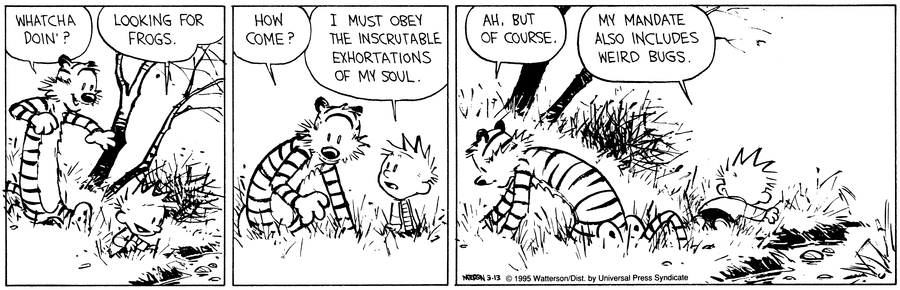
\includegraphics[width=\textwidth]{backend/ch_comic_dedication}\\
	
	\vspace{1.8cm}
	
	This thesis is dedicated to obeying the inscrutable exhortations of your soul.
	\extrafootertext{\tiny Calvin and Hobbes is the property of Mr. Bill Watterson and Andrews McMeel Syndication. This comic has been reproduced with explicit permission from Andrews McMeel Syndication.}
	}

%Details of graduation date
\graduationyear{2023}
\academicyear{2022-2023}
\graduationmonth{May}

%The abstract goes here. IISER guidelines say it should be <= 250 words.
\thesisabstract{
Population biology is built on a strong mathematical foundation developed during the Modern Synthesis. Historically, much of this foundation has been built using models of infinite populations, ignoring the effects of demographic stochasticity. Finite population models in population and quantitative genetics usually assume a fixed population size and are of limited applicability in a world where population sizes  routinely fluctuate. In this thesis, I analytically describe evolution in finite, fluctuating populations from biological first principles. Starting from a density-dependent `birth-death process’ describing an arbitrary closed population of individuals with discrete traits, I derive stochastic differential equations (SDEs) for how trait frequencies change over time. These SDEs reveal a new directional evolutionary force, `noise-induced selection’, that is particular to finite, fluctuating populations and has been largely overlooked in standard formulations of evolution. Noise-induced selection can cause deviations from neutrality and may reverse the direction of evolution predicted by infinite-population frameworks. My SDEs also recover well-known results such as the replicator-mutator equation and the Price equation in the infinite population limit, and help explain and organize several previous studies under a single theoretical framework. Finally, I extend the birth-death formalism to one-dimensional quantitative traits through a `stochastic field theory’ that yields frameworks such as Kimura's continuum-of-alleles and Lande's gradient dynamics in the infinite population limit. My work thus generalizes the formal structures of population biology to finite, fluctuating populations and predicts a new evolutionary force unique to such populations. I also discuss the implications for designing evolutionary agent-based models and empirical studies.
}

%The acknowledgements go here.
\acknowledgments{
First and foremost, I am grateful to my advisors, Prof. Vishwesha Guttal and Prof. Rohini Balakrishnan, for their masterful mentoring. The enormous academic freedom they gave me to pursue essentially whichever ideas seemed promising at the time, coupled with their readiness to provide detailed guidance whenever I asked for it, made working with them an incredibly enriching experience. Their constant focus on the bigger picture was vital to helping me see the forest when I was stuck looking at the trees. Both Vishu and Rohini are brilliant scientists and fantastic mentors, and their mentorship and guidance have deeply impacted my ways of thinking about science and mentoring. I am also grateful to all the members of the \href{https://teelabiisc.wordpress.com/}{Theoretical Ecology and Evolution lab} and the \href{https://sites.google.com/view/rohinibalakrishnanlab/home}{Animal Communication and Bioacoustics Lab} for providing a supportive and productive working environment.

I would also like to thank Prof. Sutirth Dey, my expert for this project. Sutirth provided constructive comments during the mid-year evaluation that helped me re-evaluate my project and its goals. Sutirth's brilliant course on evolution at IISER and various fascinating conversations with him and other lab members during my time as an intern at the \href{https://sites.google.com/a/acads.iiserpune.ac.in/sdlab/pbl-iiser-p}{Population Biology Lab} have been instrumental in shaping my thoughts on evolution. I am also extremely grateful to Dr. Anand Krishnan for constantly supporting me and always being there, both as a mentor and a friend, when I needed advice --- Thank you for everything.

I am grateful to many friends who made the IISER journey enjoyable. Countless long days and nights with Adithyan, Abhishek, Arjun, Chebi, Gaurav, Harshit, Manas, Milie, and Shruthi, have greatly helped me grow as a person, both intellectually and emotionally. Arjun has always been a great sounding board for my thoughts, no matter how inane, and has been very patient and supportive in more ways than I could list here. Milie is the occasional fitness friend that everyone needs, and occasionally texting her encouraged me to hit the gym at least semi-regularly even during hectic parts of the thesis project when schedules were uncertain. I am indebted to our D\&D group in general and Manas in particular for introducing me to D\&D and Critical Role, both of which were very helpful in getting through the pandemic and the thesis year. Shruthi is a constant source of cat related mental health boosts and has more generally taught me a lot about a lot during my time at IISER. I entered this project as someone who knew some mathematics and some biology but quickly realized I would benefit from reading physics papers (typically written in physics language) --- Abhishek always enthusiastically responded to my annoying physics-related questions and patiently explained physics language to me throughout the project year, and for that I am grateful. Insightful conversations about evolution with Gaurav were helpful in gaining fresh perspectives on various topics. Closer to home, Akshay and Prerana have been my closest friends since high school and continue to provide unerring and unconditional love and support. I don't know where I would be without them today.

I am also grateful to various non-human companions, canine, feline, and more exotic. The dogs and cats of ISI are more helpful to my mental health than I could possibly articulate. Even though my thesis work may seem dreadfully abstract, running after pretty animals in the Western Ghats and other wild places of India is how I even got interested in science in the first place, and I certainly wouldn't be here today if the animals weren't so fascinating :)

Finally, I am eternally indebted to my parents, Raja and Vidya. They have unfailingly supported me at every step of my life, and have nurtured and encouraged an inquisitive wonder of the world that no doubt played a vital role in helping me choose this career path. Not many parents would raise their children on Durrell and Feynman or take time out of their day to help their child find the right plant or jar for keeping an insect in the house. Upon finding out that their child has an early fascination with praying mantids and finding that there is no accessible information about the topic, not many parents would encourage their child to try and write their own source on the subject by keeping these insects at home and documenting their behavior. Upon finding out that their child was interested in snakes, not many parents would encourage this interest and actively accompany them to animal rescue centers, snake parks, and herpetology summer camps. Not many parents would be okay with their child spending weeks in the rainforest with no cellular network catching snakes and looking for frogs in the dark with a flashlight. Certainly, not many Indian parents would let their child pursue this love of animals professionally and allow them to virtually ignore the more `mainstream' entrance exams for engineering and medical colleges in favor of fully committing to the pipe dream of getting accepted by an IISER or IISc. Not many parents would provide an actively supporting environment at home for an MS project, without questioning their child's future plans or PhD application process at any stage, and just trusting that the child will figure things out. Not many parents would provide fantastic support during difficult emotional situations or not blink an eye when their child decides to grow their hair out or get a tattoo. Thank you for always believing in me and letting me make my own choices, both small and large. I love you.
}

%Add funding sources here
\funding{
I am a recipient (Registration no. SX-1711025) of the Kishore Vaigyanik Protsahan Yojana (KVPY) fellowship from the Department of Science and Technology, Government of India, and gratefully acknowledge the same for providing financial support.

The support and the resources provided by the PARAM Brahma Facility under the National
Supercomputing Mission, Government of India at the Indian Institute of Science Education
and Research (IISER), Pune are gratefully acknowledged; However, it is worth explicitly noting that while I did briefly run some scripts on the PARAM-Brahma facility that were related to my thesis project, none of the scripts or simulations run on the PARAM-Brahma supercomputer ultimately contributed to this thesis --- The main text is completely analytical, and Appendix \ref{App_examples} only uses very simple simulations that were run on my personal laptop.
}

\allowdisplaybreaks %allow align envts to go across pages   

%%%%%%%%%%%%%%%%%%%
%  The Document   %
%%%%%%%%%%%%%%%%%%%

\begin{document}
%\microtypesetup{disable}
\pagestyle{plain} %Don't make the initial frontmatter fancy

%Add the frontmatter
\thesisfront

%wrap the declaration of every new \part in the \clear and the group to ensure that the fresh page created by \part does not have a page number.
% This hack-ey workaround is from https://tex.stackexchange.com/a/191189 and is needed because \part defines \pagestyle WITHIN the definition itself and so you cannot use \thispagestyle to mess with it
\cleardoublepage
\begingroup
\makeatletter
\let\ps@plain\ps@empty
\part{Motivation \& Outline}
\endgroup

%Enable microtype from here on out
%\microtypesetup{enable}

%Implement the fancy headers for everything from here on out
\pagestyle{fancy}
\fancyhf{}
\fancyhead[LE,RO]{\thepage}
\fancyhead[CE]{\rule[-4ex]{0pt}{4ex}\footnotesize\itshape Eco-evolutionary dynamics of finite populations from first principles}
\fancyhead[CO]{\rule[-4ex]{0pt}{4ex}\footnotesize\itshape\nouppercase{\leftmark}}
\setlength{\headheight}{40pt} % as requested by fancyhdf
\renewcommand{\headrulewidth}{0pt}

\renewcommand{\chaptermark}[1]{\markboth{#1}{}} %gets rid of chapter number from header
\renewcommand{\sectionmark}[1]{\markright{#1}} %gets rid of section number from header

%From here on, we just need to import TeX files from the ind_files folder to include the actual content of the thesis

%Intro
\chapter{Introduction}
\epigraph{\justifying The theory of evolution by natural selection is an ecological theory—founded on ecological observation by perhaps the greatest of all ecologists. It has been adopted by and brought up by the science of genetics, and ecologists, being modest people, are apt to forget their distinguished parenthood}{John Harper~\citep{harper_darwinian_1967}}

%More than 150 years have passed since Charles Darwin first published \textit{Origin} (in 1859) and Ernst Haeckel first coined the term ‘ecology’ (in 1866). Today, both ecology and evolution are incredibly interdisciplinary fields, borrowing techniques and ideas from diverse areas such as computer science, statistics, economics, dynamical systems, physics, and information theory. With this development has come a cornucopia of models that try to understand biological phenomena in the language of these borrowed tools and techniques. Though many of these ideas are used to accurately describe and analyze specific systems, there is also value to formulating general models in abstract terms that only incorporate a small number of `fundamental' processes and try to capture the `essence' of a biological pattern~\citep{frank_natural_2012, vellend_theory_2016,luque_mirror_2021}. Such general organizing models are vital to theory-building~\citep{luque_mirror_2021} because they help clarify conceptual similarities and unifying factors between apparently disparate modelling frameworks, helping us seamlessly translate essential ideas from one theoretical language to another.
%
%\section{Idealization and generality}\label{idealization}
Idealization and generalization are part and parcel of science, and this is clear if one looks at the actual practice, be it theorists making unrealistic assumptions on paper to model specific phenomena or experimentalists creating artificially controlled conditions in the laboratory to test specific hypotheses~\citep{zuk_models_2018}. Indeed, some philosophers of science argued that ``the epistemic goal of science is not truth, but understanding''~\citep{potochnik_idealization_2018}, an idea generally echoed by practicing scientists~\citep{levins_strategy_1966,servedio_not_2014,zuk_models_2018,grainger_empiricists_2022}. In other words, since the world is complicated and humans are limited, general understanding inevitably comes at the cost of other desirable qualities such as the ability to make precise quantitative predictions. This is especially true for complex phenomena such as those that are the domain of ecology and evolution, where we are often not even aware of all the factors that are at play or how they interact. We thus benefit from formulating simple `general' models that provide simple qualitative predictions and help us think about the phenomena we study in a cohesive, unified framework that we can understand well~\citep{potochnik_idealization_2018,luque_mirror_2021}.   
 
A general approach need not (and often will not) be perfect or all-encompassing. As Robert MacArthur once remarked, ``general events are only seen by ecologists with rather blurred vision. The very sharp-sighted always find discrepancies and are able to see that there is no generality, only a spectrum of special cases”~\citep{kingsland_modeling_1985}. MacArthur was speaking primarily about biological generalities and special cases, but in a related vein, if our language of choice for expressing our general events is mathematics, making any non-trivial observations in complex fields such as ecology and evolution often requires \emph{mathematical} approximations and idealizations that may exclude or underplay several `low-level' model-specific details in favor of a more general description at a `higher' level achieved in some limit that only contains a small number of `model-independent' quantities, often derived from first principles. Formulating and studying such general frameworks can be greatly beneficial as an aid to thinking, sometimes precisely \emph{because} `blurry eyed' thinking that begins from a small set of fundamental first principles and only looks for general broad-brush regularities can be much more insightful than accounting for every little detail or special case. The success of such an approach is perhaps best illustrated by the success of statistical mechanics in physics - Statistical mechanics was essentially born from the idea that various useful statements about systems with many moving parts can be made without the need for knowing the excruciating details of every single moving part, and indeed, starting from first principles, this sort of explicitly `blurry-eyed' thinking that only looked at approximate properties was shown to be able to recover the phenomenological laws of thermodynamics as \emph{statistical} laws.

%In population ecology, Vellend has argued that conceptual synthesis requires
%``shifting the emphasis away from an organizational structure based on the useful lines of
%inquiry carved out by researchers, to one based on the fundamental processes that underlie community dynamics and patterns''~\citep{vellend_theory_2016}. Vellend's assertion is based on the
%fact that population genetics has managed to come up  with reasonably comprehensive theory due to its focus on the abstract `high-level’ processes of selection, mutation, drift, and
%gene flow (see section \ref{sec_history} below) instead of the myriad `low-level' processes that may be responsible for generating them. In contrast, he believes that practitioners of community ecology often focus on specific `low-level' processes such as predation rate, limiting resources (R\textsuperscript{*}), storage effects,
%priority effects, senescence, and niche partitioning, leading to a plethora of models (see Table
%5.1 in~\cite{vellend_theory_2016} for an in-exhaustive list of 24 such models) and the conclusion that
%community ecology `is a mess'. Vellend instead proposes speaking about ecological theory in terms of the `high-level’ processes of selection, ecological drift (demographic stochasticity), speciation,
%and dispersal, in direct analogy with the `high-level' processes of selection, genetic drift, mutation, and gene flow respectively in population genetics. Without dwelling on the practicality of such an organization, which has been written about in great detail in~\cite{vellend_theory_2016}, I will simply note that such an organization and broad analogy at the very least seems somewhat plausible from a theoretical viewpoint, and is desirable for providing a cohesive theoretical underpinning for speaking about various hypotheses and ideas in community ecology and how they relate to each other. This is especially relevant given the increasing recognition that population ecology and evolutionary dynamics (Here I really mean the theoretical frameworks of population genetics + quantitative genetics\footnote{Though one could perhaps argue that all evolutionary phenomena should be captured in this sort of framework for some sufficiently general definition of the words `population', `quantitative', and `genetics'. In Michael Lynch's words, ``Nothing in evolution makes sense except in the light of population genetics''~\citep{lynch_origins_2007}. I don't know if this is an extreme view, though, which is why these sentences are in a footnote :)}) are perhaps not as neatly separated as many early architects of the fields had thought~\citep{coulson_putting_2006,metcalf_why_2007,schoener_newest_2011,kokko_can_2017,lion_theoretical_2018,govaert_eco-evolutionary_2019,svensson_eco-evolutionary_2019,hendry_critique_2019}.

\section{A (very, very) brief summary of high-level modelling frameworks in population biology}\label{sec_history}

In biology, arguably the greatest such general organizing framework was the idea of evolution by natural selection as synthesized from myriad detailed observations by Charles Darwin. Theoretical population genetics has also had a long-standing tradition in building general organizing frameworks that `abstract away' some biological specificities in favor of a small number of `fundamental' notions like selection and mutation which act on a small number of `fundamental' quantities like fitness. The description of evolution in these general terms was first laid out in formal mathematical terms during the Modern Synthesis by authors such as Wright, Fisher, and Haldane, an extremely successful venture that unified two major schools of thought --- Mendelian genetics and Darwinian evolution --- that were, at the time, considered to be incompatible~\citep{provine_origins_2001}. It is currently thought that this unification would have been unlikely or would have taken much longer if the architects of the Modern Synthesis had stuck to verbal arguments instead of working with formal models in explicitly mathematical terms~\citep{walsh_darwins_2014}. 

The most general mathematical framework we have for evolutionary population biology is the Price equation. Indeed, much like statistical mechanics in physics, the Price equation is derived from a small number of very general first principles and is able to recover several standard equations as special cases. The Price equation partitions changes in population composition into multiple terms, each of which lends itself to a straightforward interpretation in terms of `high-level' evolutionary forces such as selection and mutation, thus providing a useful conceptual framework for thinking about how populations change over time~\citep{frank_natural_2012}. However, the greater complexity of ecology and evolution relative to physics has meant that the generality of the Price equation comes with a much bigger cost in predictive power - the Price equation in its most general formulation is dynamically insufficient\footnote{Since this is not very standard nomenclature outside theoretical biology and related fields: `Dynamically insufficient' means that the equation cannot be iterated, or presented in the form of a difference equation $x_{t+1} = F(x_t)$ or a differential equation $\dot{x} = F(x)$. Thus, we cannot predict a dynamic `trajectory' given an initial condition $x_0$. The term `insufficient' is to indicate that the equation requires `complete' information to be true and only relates two quantities `in retrospect'. It is thus `insufficient' for prediction. In our case, in its most general setting, the Price equation is usually formulated in a way that partitions a \emph{given} amount of phenotypic change between two populations (usually but not necessarily the same population at two different times) into change due to selection, transmission bias, etc., rather than \emph{predicting} a trajectory for how much phenotypic change will occur at various future times based on the \emph{current} phenotypic distribution.}~\citep{van_veelen_use_2005,frank_natural_2012,luque_one_2017}. However, this need not be the case, and indeed, several authors have put forth more predictive versions of the Price equation by moving to a continuous time differential equation framework in which the Price equation is dynamically sufficient but manifests in a slightly less general form~\citep{page_unifying_2002,lion_theoretical_2018,day_price_2020}.

These general formulations are still often very difficult to coax concrete quantitative predictions from, but they do lend themselves to simple biological interpretation, and in the dynamically sufficient formulations, often provide \emph{qualitative} predictions. These qualitative predictions, as well as the decomposition of terms in the original Price equation, are useful primarily for their generality --- The Price equation gives us a clear idea of which evolutionary forces operate in which systems and when in an almost entirely `model-independent' language~\citep{okasha_evolution_2006,frank_natural_2012,queller_fundamental_2017,luque_one_2017}. It also leads to a small number of simple yet insightful `fundamental theorems' of population biology~\citep{queller_fundamental_2017, lion_theoretical_2018, lehtonen_price_2018} that serve a similar function, and unifies several various seemingly disjoint formal structures of evolution under a single theoretical banner~\citep{ lehtonen_price_2020, luque_mirror_2021}.

The success of the Modern Synthesis illustrates the value of formulating abstract mathematical models that only provide a `high-level' description of the fundamental processes required to capture the essence of biological evolution~\citep{provine_origins_2001,walsh_darwins_2014}. However, the evolutionary play that architects of the Modern Synthesis studied famously unfolds in the ecological theatre~\citep{hutchinson_ecological_1965}. Thus, quantities like fitness are not truly fundamental but instead emerge as the net result of various ecological interactions, tradeoffs, and constraints~\citep{metz_how_1992}, a fact that can have important consequences for evolution~\citep{coulson_putting_2006,schoener_newest_2011, kokko_can_2017}. Trying to understand such `eco-evolutionary feedbacks' or `eco-evolutionary dynamics' has sprouted a rich body of literature under the broad heading of `evolutionary ecology' that has greatly enriched our understanding of biological populations~\citep{coulson_putting_2006,metcalf_why_2007,schoener_newest_2011,brown_why_2016,kokko_can_2017,lion_theoretical_2018,govaert_eco-evolutionary_2019,svensson_eco-evolutionary_2019,hendry_critique_2019}. Several major theoretical frameworks in the slightly more general setting of eco-evolutionary dynamics --- such as evolutionary game theory and adaptive dynamics --- as well as the standard equations of population genetics and quantitative genetics, can still be recovered (in a very general sense) as special cases of a slightly reformulated version of the Price equation~\citep{page_unifying_2002,lion_theoretical_2018}.

One of the general guiding principles of much of this mathematization has been the assumption that incorporating the reality of finite population sizes into models leads to no major qualitative differences in behavior, only `adding noise' or `blurring out' the predictions of simpler infinite population models~\citep{page_unifying_2002}. Consequently, several major theoretical frameworks in the field, such as adaptive dynamics, are explicitly formulated in deterministic terms at the infinite population size limit. However, this assumption is largely unjustified, and since populations in the real world are finite and stochastic, checking whether stochastic models differ from their deterministic analogs is vital to furthering our understanding of the fundamentals of population biology~\citep{hastings_transients_2004, coulson_skeletons_2004, shoemaker_integrating_2020}. Today, we increasingly recognize that incorporating the finite and stochastic nature of the real world routinely has much stronger consequences than simply `adding noise' to deterministic expectations~\citep{boettiger_noise_2018}, with important consequences for both ecological~\citep{schreiber_does_2022} and evolutionary~\citep{delong_stochasticity_2023} theory. In ecology and evolution, stochastic models need not exhibit phenomena predicted by their deterministic analogues~\citep{proulx_what_2005, johansson_will_2006, claessen_delayed_2007,  wakano_evolutionary_2013, debarre_evolutionary_2016, johnson_two-dimensional_2021}. In addition, they exhibit novel phenomena not predicted by the deterministic approximations~\citep{rogers_demographic_2012, rogers_spontaneous_2012, rogers_modes_2015, veller_drift-induced_2017, delong_stochasticity_2023}, for example, even completely `reversing' the predictions of deterministic models~\citep{houchmandzadeh_selection_2012,houchmandzadeh_fluctuation_2015,constable_demographic_2016,mcleod_social_2019}.

Studies of neutral or near-neutral dynamics in population and quantitative genetics usually do take stochasticity seriously, explicitly modeling finite populations that follow stochastic dynamics. Unfortunately, the classic or standard stochastic models in both population genetics~\citep{fisher_genetical_1930,wright_evolution_1931, moran_random_1958, kimura_diffusion_1964} and quantitative genetics~\citep{crow_introduction_1970, lande_natural_1976} typically assume a fixed total population size, thus restricting their validity in a world where population sizes routinely fluctuate. Those models which study evolution in populations with non-constant size usually impose deterministic and typically phenomenological rules for how the total population size must vary~\citep{kimura_probability_1974,ewens_probability_1967,otto_probability_1997, engen_fixation_2009, waxman_unified_2011}. These rules further usually do not depend on population composition. Such models are thus somewhat artificial since demography and population size are forced to be independent quantities even though this is obviously not the case in natural populations, where population size is a `bulk' property whose value emerges from an intricate interplay of the individual-level demographic processes of birth and death~\citep{metcalf_why_2007,doebeli_towards_2017}. Notably, the most general framework we have, the Price equation, is typically formulated in a deterministic setting ~\citep{page_unifying_2002,frank_natural_2012,queller_fundamental_2017,lion_theoretical_2018,day_price_2020} that ignores stochasticity (but see~\cite{rice_stochastic_2008,rice_universal_2020} for a discrete time formulation that is stochastic but, as far as I can tell, is dynamically insufficient, just like the original formulation of the Price equation). Since real-life populations are stochastic, finite, and of non-constant population size, this is somewhat of a problem, since we know that such deterministic approximations that may not capture important dynamics of the real systems of interest.

Incorporating stochasticity into deterministic systems is a tricky business, and, if done in a phenomenological manner by adding noise to a `deterministic skeleton'~\citep{coulson_skeletons_2004} in an ad-hoc fashion, can lead to models that are not self-consistent~\citep{strang_how_2019}. Further, this procedure of adding noise in an ad-hoc manner provides no insight into the mechanistic factors actually responsible for the stochasticity in the first place. Stochastic individual-based models, in which (probabilistic) rules are specified at the level of the individual and population level dynamics are systematically derived from first principles, are self-consistent, much more natural, and can fundamentally differ from the predictions made by simply adding noise terms to a deterministic model~\citep{black_stochastic_2012,strang_how_2019}. Formulating the fundamental formal structures of evolutionary biology in terms of the mechanistic demographic processes of birth and death at the individual level is also greatly desirable for biological reasons~\citep{metcalf_why_2007,geritz_mathematical_2012} because `all paths to fitness lead through demography'~\citep{metcalf_all_2007}. In other words, since demographic processes such as birth and death rates explicitly account for the ecology of the system, they can more accurately reflect the complex interplay between ecological and evolutionary processes and provide a more fundamental mechanistic description of the relevant evolutionary forces and population dynamics~\citep{doebeli_towards_2017}. In this thesis, I present a formulation of population dynamics constructed from mechanistic first principles grounded in individual-level birth and death. The mathematical formalism itself is very general and applies equally to the `high level' forces of population genetics and the `high level' forces of community ecology as postulated by~\cite{vellend_theory_2016}, though I will mostly stick to the population genetics interpretation in my discussions.

\section{A very brief outline of the rest of this thesis}
This section provides a bullet-point chapter-wise outline for convenience. A more detailed outline of the thesis, with explanations of the technical content covered, originality, etc., is provided in the next section.

This thesis develops a mathematical formalism for describing finite fluctuating populations from first principles and is structured as follows. The rest of this thesis is divided into two parts. Part \ref{part_theory} provides the complete formalism in all its gory mathematical detail, but in a (hopefully) accessible pedagogical style. Part \ref{part_summary} then (re)presents some major results from part \ref{part_theory} and discusses their implications and connections with previous studies. Appendix \ref{App_examples} presents some concrete examples of models for clarity regarding the major ideas.

\begin{itemize}
		\item Chapter \ref{chap_math_background} provides the necessary mathematical background and provides a toy example studying the size of a population of identical individuals that illustrates the major ideas used. If I am required to shoehorn this thesis into a `intro-methods-results-discussion' format, then chapter \ref{chap_math_background} can be thought of as providing a mathematical `introduction' and illustration of the `methods' that will be used (in chapter \ref{chap_BD}) and generalized (in chapter \ref{chap_infD_processes}) in a biological context to get `results'.
		\item Chapter \ref{chap_BD} develops a formalism for describing the evolution of finite fluctuating populations of individuals that come in arbitrarily many `types' which vary in a \emph{discrete} character. This yields equations that generalize the classic Price equation and replicator-mutator equation to finite fluctuating populations.
		\item Chapter \ref{chap_infD_processes} extends the ideas developed in chapter \ref{chap_BD} to populations that vary in a single one-dimensional \emph{quantitative} character and derives a so-called `stochastic field theory' that describes evolution in such populations. This also results in some mathematical equations that may be of independent interest to physicists and applied mathematicians.
		\item Chapter \ref{chap_unification} provides a technical summary of the major results by deriving three important stochastic differential equations. These are equations for type frequencies, the population mean value of an arbitrary type-level quantity, and the population variance of an arbitrary type-level quantity, and respectively generalize the replicator-mutator equation, the Price equation, and \cite{lion_theoretical_2018}'s variance equation to finite, stochastically fluctuating populations. These equations predict a directional evolutionary force called `noise-induced selection' that is only seen in finite, fluctuating populations. Some implications for social evolution and community ecology are discussed. I also briefly discuss the field equation formalism I develop in chapter \ref{chap_infD_processes}.
		\item Chapter \ref{sec_disc} provides a quick summary of the major results and discusses biological implications, connections with previous studies, and opportunities for future work. This chapter has no equations (!). Thus, readers who do not want any mathematical equations can skip all other chapters and directly read chapter \ref{sec_disc} if they are interested only in the final results and takeaways. 
\end{itemize}
\section{A more expanded outline of the rest of this thesis}

Chapter \ref{chap_math_background} provides the basic mathematical background required and illustrates the major ideas that we will use. To facilitate readership by a broad audience, I only assume passing familiarity with calculus (derivatives, integrals, Taylor expansions) and probability. Familiarity with stochastic calculus is helpful for some sections but is not required, and I present a brief introduction to the relevant notions from both Markov theory and stochastic calculus in section \ref{sec_math_background}. In section \ref{sec_1D_processes}, I present a toy example of tracking population size of a population of identical individuals in section. I introduce a description of the system via a `master equation', and then conduct a `system-size expansion' to obtain a Fokker-Planck equation for the system, thus illustrating all the major tools required. For completeness, I also conduct a weak noise approximation to arrive at a so-called `linear' Fokker-Planck equation that can be solved exactly to arrive at a closed-form solution.

Chapter \ref{chap_BD} deals with the evolution of discrete traits. In this case, the system is finite-dimensional, since we can completely specify the state of the system by simply listing out the number of individuals of each type in a vector. I introduce a general multivariate process to describe the evolution of discretely varying traits, and use the system size expansion to arrive at a continuous description of change in trait frequencies as an SDE under mild assumptions on the functional forms of the birth and death rates. Unlike many classic stochastic formulations in evolutionary theory~\citep{fisher_genetical_1930,wright_evolution_1931,moran_random_1958,crow_introduction_1970, lande_natural_1976,kimura_probability_1974}, I do not assume a fixed (effective) population size and instead allow the total population size to be a natural emergent property from the demographic processes of birth and death. I show that the deterministic limit of this process is the well-known replicator-mutator equation (or equivalently, the dynamic version of the Price equation), thus establishing the microscopic basis of well-known equations from stochastic first principles. I also illustrate some general predictions that can be made using the weak noise approximation for the sake of completeness.

While the mathematics of chapter \ref{chap_BD} is standard and well-understood, it has, to the best of my knowledge, not been applied before in the generality and context we use here. Several specific models of specific systems do use these mathematical techniques, but these papers are often written assuming familiarity with notions in physics and/or mathematics and thus may not be very accessible to theoretical ecologists who do not have formal training in these subjects (but see~\cite{czuppon_understanding_2021} for a recent pedagogical review on the general approach applied to Wright-Fisher and Moran processes, where total population size is constant). As such, chapters \ref{chap_math_background} and \ref{chap_BD} together also serve as a tutorial and technical introduction to some theoretical ideas: For ecologists, the chapter introduces `system size expansions' and illustrates their use in a general setting, and can be seen as a tutorial on modelling finite populations analytically with minimal assumptions; For population geneticists, the chapter illustrates how system-size approximations (`diffusion approximations' in the population genetics literature) can be carried out without assuming a constant (effective) population size and how this generalization has important consequences for the evolutionary forces at play; For physicists and applied mathematicians, the chapter presents a study of the consequences of applying the system-size expansion to the kind of density-dependent birth-death processes that are widely applicable in ecology and evolution - Unlike many physical systems, though demographic processes like birth and death over ecological timescales are usually formulated in terms of population numbers or densities, predictions in evolution are typically in terms of frequencies of types, and this fact has subtle consequences that can be overlooked if one only works with densities, as is often done in physics studies of eco-evolutionary systems.

Chapter \ref{chap_infD_processes} introduces a function-valued process to model the evolution of quantitative traits such as body size, which can take on uncountably many values. This function-valued process can then also be analyzed via an analog of the system-size approximation to arrive at a `functional' Fokker-Planck equation in which derivatives are replaced by functional derivatives. I show that classic equations from quantitative genetics such as Kimura's cotinuum-of-alleles model~\citep{kimura_stochastic_1965} and Lande's gradient dynamics~\citep{lande_quantitative_1982} can be derived as the infinite population limit of this stochastic process. I also conduct a weak noise approximation to arrive at a linear functional Fokker-Planck equation that can be analyzed for specific systems as required. Unlike the systems studied in Chapter \ref{chap_BD}, formalizing the study of the kind of processes we study in Chapter \ref{chap_infD_processes} is an active area of mathematical research~\citep{carmona_stochastic_1999,da_prato_stochastic_2014,prevot_concise_2007,liu_stochastic_2015,bogachev_fokker-planck-kolmogorov_2015,balan_gentle_2018} and the mathematics itself is far from settled.

Chapter \ref{chap_infD_processes} generalizes the work of Tim Rogers and colleagues~\citep{rogers_demographic_2012,rogers_spontaneous_2012,rogers_modes_2015} to a wide class of eco-evolutionary systems, and to the best of my knowledge, has never been presented in full generality before. Mathematically, chapter \ref{chap_infD_processes} presents heuristic, accessible alternatives to the rigorous tools of martingale theory and measure-valued branching processes that are usually employed to describe the evolution of quantitative traits~\citep{champagnat_unifying_2006,etheridge_mathematical_2011, week_white_2021} by generalizing the idea of a system size expansion of density-dependent (finite-dimensional) birth-death processes to the infinite-dimensional case using the notion of functional differentiation. Biologically, Chapter \ref{chap_infD_processes} provides `stochastic field equations' that describe the dynamics of one-dimensional quantitative traits in finite populations and illustrates that these equations are consistent with well-known formalisms in quantitative genetics at the infinite population limit.

Part \ref{part_summary} summarizes the major results of the formalism developed in Part \ref{part_theory} and presents some simple equations that can be argued to be `fundamental equations' of population biology in the sense of~\cite{queller_fundamental_2017}, and together form a `unifying perspective' in the sense of~\cite{lion_theoretical_2018}. These equations reduce to well-known results such as the Price equation, the replicator-mutator equation from evolutionary game theory, and Fisher's fundamental theorem from population genetics in the infinite population limit. For finite populations, these same equations predict a new evolutionary force, `noise-induced selection', that has still not found its way into the standard formal canon of evolutionary biology and whose significance is only recently being recognized~\citep{constable_demographic_2016,mcleod_social_2019,mazzolini_universality_2022, kuosmanen_turnover_2022}. Implications of noise-induced selection are also discussed in part \ref{part_summary}. Readers who are okay with mathematical equations but do not want any intermediate derivations (or just trust my math) can skip to Chapter \ref{chap_unification} for the major equations that emerge as being important, though I strongly encourage working through the entire formalism properly if possible. Readers who are averse to or do not care for equations can safely skip to Chapter \ref{sec_disc} directly for the major takeaways of this thesis.



%The 'meat': Methods, results, theory, etc.
\cleardoublepage
\begingroup
\makeatletter
\let\ps@plain\ps@empty
\part{Theory}\label{part_theory}
\endgroup

\chapter{Mathematical background and an expository example}\label{chap_math_background}
\epigraph{\justifying Like most mathematicians, he takes the hopeful biologist to the edge of a pond, points out that a good swim will help his work, and then pushes him in and leaves him to drown.}{Charles Elton, speaking about Lotka~\citep{elton_eppur_1935}}

Theorists are often accused of presenting somewhat intuitive ideas in a highly inaccessible formalism that discourages those unfamiliar with the required mathematics. Indeed, many models that use the kind of stochastic processes I use in this thesis assume familiarity with stochastic calculus or Markov theory, or at the very least a willingness to `fill in the blanks' between major results of the calculations. In an attempt to make the ideas I use more accessible to a broader audience, I will use this expository chapter to present a pedagogical summary of the basic mathematical tools required, and present a toy model tracking the population size of a population of identical individuals as an example of the major ideas used.

\section{Mathematical Background}\label{sec_math_background}

Here, I provide a brief, informal introduction to basic notions in stochastic processes that will be helpful for some technical portions of this thesis. Interested readers looking for a more comprehensive source can refer to standard mathematics texts such as~\cite{oksendal_stochastic_1998} or~\cite{karatzas_brownian_1998} for a more rigorous treatment of the mathematical foundations, or physics-style texts such as~\cite{gardiner_stochastic_2009} or~\cite{van_kampen_stochastic_1981} for useful tools and techniques to study real systems.

\subsection{Birth-death processes}
Mathematically, a birth-death process is a so-called `continuous-time Markov chain' in which only transitions between local states are allowed. In other words, a birth-death process is a stochastic process unfolding in continuous time such that
\begin{itemize}
	\item The process is `Markov', meaning that the future is statistically independent of the past given the present. In more mathematical terms, if the value of the stochastic process at time $t$ is given by $X_t$, $\mathbb{P}(\cdot | E)$ denotes probability conditioned on $E$, and $u < s \leq t$, then
	\begin{equation*}
	\mathbb{P}(X_t | X_s, X_u) = \mathbb{P}(X_t | X_s)
	\end{equation*}
	This equation is simply saying that if we have the information about the state of a process at time $s$, then we do not gain any more predictive power about the process at a future time $t$ if we have additional knowledge about the process from some past time $u < s$. A series of tosses of a fair coin is a simple example of a Markov process, since knowing whether a coin landed on heads during a previous toss does not change your predictive power about whether the coin will land on heads the next time you toss it.
	\item Direct transitions must be `local'. Mathematicians usually reserve the phrase `birth-death process' to processes that take values in the non-negative integers $\{0,1,2,3,4,\ldots\}$. In this case, only direct transitions from $n$ to $n \pm 1$ are allowed to occur. Biologically, this is saying that we observe the population on a fine enough timescale that the probability of two or more births/deaths occurring at the exact same time is very low and we can disallow it entirely in our models. The conditions for higher dimensional birth-death processes look similar.
\end{itemize}
Since these processes unfold in continuous time, they are characterized not by transition probabilities but by transition \emph{rates}, which can be thought of as the probability of transition `per unit time'. The quantity of interest is usually the probability of being in a particular state at a given point in time. The entire birth-death process can be described in terms of such a quantity, through a so-called `Master equation'. The master equation is a partial differential equation (PDE) for the probability of being in a given state at a given time, However, in all but the simplest cases, we can't actually solve this PDE, because it is simply too hard. The primary source of difficulty is non-linearity in the transition rates and the fact that transitions occur in discrete, discontinuous `jumps'. It is much easier to describe and analyze systems by using tools from stochastic calculus and partial differential equations, as we describe below.

\subsection{SDEs and the Fokker-Planck equation}\label{intro_SDE}
Stochastic systems which change continuously (in the state space) can be described in terms of a `stochastic differential equation' (SDE), which here is interchangeable with the phrase `It\^o process'. An SDE for a stochastic process $\{X_t\}_{t \geq 0}$ is an equation of the form
\begin{equation}
\label{ito_SDE_integral}
X_t = \int\limits_{0}^{t} F(s,X_s)ds + \int\limits_{0}^{t} G(s,X_s)dW_s
\end{equation}
where $F(t,x)$ and $G(t,x)$ are `nice' functions\footnote{For the mathematically oriented reader, there are two requirements: Firstly, we require the functions to have `linear growth', meaning that we can find a constant $C > 0$ such that $\|F(t,x)\| + \|G(t,x)\| \leq C(1+\|x\|)$ for every $x \in \mathbb{R}^{d}$ and $t > 0$. We also require `Lipschitz continuity', which means that we can find a constant $L > 0$ such that $\|F(t,x) - F(t,y)\| + \|G(t,x)-G(t,y)\| \leq L\|x-y\|$ for every pair $x,y \in \mathbb{R}^d$ and $t > 0$. Here, $\|\cdot\|$ denotes the natural norm on the space under consideration and for our cases will usually be the Euclidean norm. For biological systems, both of these conditions will usually be satisfied, and so we assume going further that all our SDEs are always well-defined and admit solutions.} In the physics literature, $F$ and $G$ are often called the `drift' and `diffusion' of the process respectively. However, we will not use this terminology here due to  potential confusion with genetic drift (which actually corresponds to the `diffusion' in the physics terminology). $W_t$ is the so-called `Wiener process' or `standard Brownian motion'. Named after the botanist Robert Brown (who was looking at the random erratic motion of pollen grains in water under a microscope), $\{W_t\}_{t \geq 0}$ is a stochastic process that is supposed to model `random noise' or `undirected diffusion' of a particle. If one imagines $W_t$ as recording the position of a small pollen grain at time $t$, then $W_t$ can be formally thought of as a process that has the following properties:
\begin{itemize}
	\item It starts at the origin, \emph{i.e} $W_0 = 0$. This is a harmless assumption made for convenience and amounts to a choice of coordinate system.
	\item It moves continuously, without sudden jumps across regions of space, \emph{i.e} the map $t \to W_t$ is continuous. This simply says that our pollen grain moves short distances in short intervals of time.
	\item The future movement is independent of past history. That is, given times $u < s < t$, the displacement $W_t - W_s$ is independent of the past position $W_u$.
	\item The movement is directionless and random, and displacement is normally distributed. More precisely, given two times $s < t$, the displacement $W_t - W_s$ follows a normal distribution with a mean of $0$ (this is the `directionless' part) and a variance of $t-s$ (this is the `random' part).
\end{itemize}
It can then be shown that since the motion is equally likely to be in any direction, the expected position at any point of time is the same as the initial position, \emph{i.e} $\mathbb{E}[W_t | W_0] = W_0 = 0$.

The second integral in equation \eqref{ito_SDE_integral} is It\^o's `stochastic integral', and is to be interpreted in the following sense: Fix a time $T > 0$. For any $n\geq2$, let $\Pi_n = \{t_1,t_2,\ldots,t_n\}$ be a partition of the interval $[0,T]$. In other words, $\Pi_n$ divides $[0,T]$ into $n$ slices of the form $[t_i,t_{i+1}]$ such that $0 = t_0 < t_1 < t_2 < \ldots < t_n = T$. Then, the (It\^o) stochastic integral from $0$ to $T$ can be thought of as:
\begin{equation*}
\int\limits_{0}^{T} G(s,X_s)dW_s \coloneqq \lim_{n \to \infty} \sum\limits_{t_i \in \Pi_n}G(t_i,X_{t_i})(W_{t_{i+1}}-W_{t_i})  
\end{equation*}
That is to say, it is obtained by making successively finer partitions of the form $[t_i,t_{i+1}]$, and then computing the `area of the rectangle' formed with $W_{t_{i+1}}-W_{t_i}$ and $G(t_i,X_{t_i})$ as sides. This should look similar to the classic Riemann integral, with the uniform width $t_{i+1}-t_i$ of the Riemann integral replaced by a random width corresponding to the random displacement of a Brownian particle during the uniform time interval $[t_i,t_{i+1}]$.

Equation \eqref{ito_SDE_integral} is often represented in the compact form:
\begin{equation}
\label{ito_SDE_diff}
dX_t = F(t,X_t)dt + G(t,X_t)dW_t
\end{equation}
. The physics literature also often uses the `Langevin form':
\begin{equation}
\label{ito_langevin}
\frac{dx}{dt} = F(t,x) + G(t,x)\eta(t)
\end{equation}
where $\eta(t)$ is supposed to be `Gaussian white noise', defined indirectly such that $\int_0^{t}G(s,x)\eta(s)ds$ behaves identically to $\int_0^{t}G(s,X_s)dW_s$. However, it is important to remember that these are both purely formal expressions - Equation \eqref{ito_SDE_diff} is meaningless on its own and is really just shorthand for equation \eqref{ito_SDE_integral}, which is well-defined as explained above; Equation \eqref{ito_langevin} is even worse, because the Brownian motion is known to be non-differentiable, and as such, $\eta(t)$ cannot really exist - Both equations are thus to be interpreted as shorthand for equation \eqref{ito_SDE_integral}, which formally `makes sense'. SDEs are convenient because they satisfy several `nice' analytical properties. For example, using the fact that the Brownian motion has no expected change in value (\emph{i.e} $\mathbb{E}[W_t | W_0] = W_0 = 0$), it can be shown\footnote{We can actually prove something stronger: We can show under rather mild regularity assumptions on $X_t$ and $G(t,x)$ that the stochastic integral is a continuous square-integrable martingale starting at the origin - This means that the map $t \to \int_0^{t}G(s,X_s)dW_s$ is continuous, starts at the origin, and always has an expectation value of $0$.} that the stochastic integral also has an expectation value of $0$ for all $t$, \emph{i.e}:
\begin{equation*}
\mathbb{E}\left[\int\limits_{0}^{t} G(s,X_s)dW_s \bigg{|} X_0\right] = 0
\end{equation*}
Using this, and the fact that the future path of the Brownian motion itself is independent of its history, one can derive the following `notational algebra table' for manipulating products of formal expressions of the form \eqref{ito_SDE_diff}:
\\
\begin{center}
	\begin{tabularx}{0.4\textwidth}{ 
			| >{\centering\arraybackslash}X 
			| >{\centering\arraybackslash}X 
			| >{\centering\arraybackslash}X | }
		\hline
		& $\mathbf{dt}$ & $\mathbf{dW_t}$ \\
		\hline
		$\mathbf{dt}$ & $0$  &  $0$ \\ 
		\hline
		$\mathbf{dW_t}$ & $0$  & $dt$ \\
		\hline
	\end{tabularx}
\end{center}
which becomes very useful for formal manipulation. One important consequence of this table is that we can no longer rely on the normal rules of calculus when dealing with stochastic integrals. In regular calculus, if we had a quantity $x(t)$ satisfying
\begin{equation*}
	\frac{dx}{dt} = f(x) + g(x)
\end{equation*}
for two `nice'\footnote{We just need the solution $x(t)$ to be a continuous function} real functions $f$ and $g$, then, given any real function $h$, we can calculate how teh quantity $h(x)$ changes using the chain rule of differentiation, which says that
\begin{equation*}
\frac{dh}{dt} = \frac{dh}{dx}\frac{dx}{dt} = h'(x)f(x) + h'(x)g(x)
\end{equation*}
\emph{i.e.}
\begin{equation*}
dh =  h'(x)f(x)dt + h'(x)g(x)dt
\end{equation*}
Naively, we may expect the same logic to still hold true for one-dimensional It\^o processes of the form
\begin{equation*}
dX_t = F(X_t)dt + G(X_t)dW_t
\end{equation*}
with $gdt$ simply being replaced by $GdW_t$ on the RHS. However, this does not work. The correct relation is instead given by 
\emph{It\^o's formula}\footnote{It\^o's formula also additionally requires $h \in C^2(\mathbb{R})$, meaning that $h$ is continuous and the first and second derivatives of $h$ exist and are also continuous}:
\begin{equation*}
dh(X_t) = h'(X_t)F(X_t)dt + h'(X_t)G(X_t)dW_t  + \frac{h''(X_t)}{2}G^2(X_t)dt 
\end{equation*}
There is now an extra $h''(X_t)G^2(X_t)/2$ term that does not exist in the deterministic setting(!). Using It\^o's formula and some simple algebra, one can then show that given any process $X_t$ taking values in $\mathbb{R}$ satisfying the SDE \eqref{ito_SDE_diff}, the associated probability density $P(x,t)$ of finding the process in a state $x \in \mathbb{R}$ satisfies the PDE
\begin{equation}
\label{ito_FPE}
\frac{\partial P}{\partial t}(x,t) = -\frac{\partial}{\partial x}\{F(t,x)P(x,t)\} + \frac{1}{2}\frac{\partial^2}{\partial x^2}\{(G(t,x))^2P(x,t)\}
\end{equation}
I present a simple informal derivation in Appendix \ref{App_SDE_FPE} for the sake of completeness. Equation \eqref{ito_FPE} is called the `Fokker-Planck equation' in the physics and applied mathematics literature~\citep{gardiner_stochastic_2009} and is often called the `Kolmogorov forward equation' in the population genetics~\citep{ewens_mathematical_2004} and pure mathematics~\citep{oksendal_stochastic_1998} literature. As I explain in Appendix \ref{App_SDE_FPE}, the Fokker-Planck equation can be viewed as a `conservation law' for probability that mathematically expresses the common-sense observation that the sum (or integral) of probabilities over the entire state space cannot change over time (since it must always equal 1). If the function $G$ is independent of $x$, it comes out of the derivatives in equation \eqref{ito_FPE}, and the resultant Fokker-Planck equation is said to be `linear' (and is much easier to solve). This link between SDEs and Fokker-Planck equations goes both ways: One can show that every stochastic process with a probability density described by a Fokker-Planck equation of the form \eqref{ito_FPE} corresponds to the solution of an SDE of the form \eqref{ito_SDE_diff}, though the proof is much more technical and will not be discussed here. This two-way correspondence proves to be extremely useful, as one approach often works for applications in which the other fails. This correspondence makes it greatly desirable to be able to describe our stochastic process of interest as either the solution to an It\^o SDE of the form \eqref{ito_SDE_diff} or as the solution to a Fokker-Planck equation of the form \eqref{ito_FPE}. System-size expansions facilitate such a description for birth-death processes.

\subsection{Density-dependence and the intuition for system-size expansions in ecology}
The fundamental idea behind the system-size expansion relates to the nature of the jumps between successive states of a birth-death process. In most situations in ecology, at an individual level, births and deaths of individuals are affected by local population density and not directly by the total population size. Despite this, the jumps themselves occur in terms of the addition (birth) or removal (death) of a \emph{single individual} from the population. If there are many individuals, each individual contributes a negligible amount to the density, and thus, the discontinuous jumps due to individual-level births or deaths can look like a small, \emph{continuous} change in population density. This is the essential idea behind the system-size expansion. The name derives from the formalization of this idea as a change of variable from the discrete values $\{0,1,2,\ldots,n-1,n,n+1,\ldots\}$ to the approximately continuous values $\{0,1/K,2/K,\dots,x-1/K,x,x+1/K,\ldots\}$ by the introduction of a `system size parameter' $K$. In ecology, this parameter will be some fundamental limit on resources, such as habitat size or carrying capacity. In physics and chemistry, it is usually the total volume of a container in which physical or chemical reactions take place. When $K$ is large, the fact that transitions occur in units of a small value $1/K$ can be exploited via a Taylor expansion of the transition rates in the Master equation, which then yields a Fokker-Planck equation upon neglecting higher order terms. A similar approximation is well-known (ever since Fisher) in theoretical population genetics, where it goes by the name of the `diffusion approximation'\citep{ewens_mathematical_2004} or `continuum limit'~\citep{czuppon_understanding_2021}, and has been heavily used by Kimura~\citep{crow_introduction_1970} in his stochastic models. However, the population genetics version of the approximation usually either relies on total population size being fixed~\citep{crow_introduction_1970, lande_natural_1976,ewens_mathematical_2004} or is conducted in an ad-hoc manner without specifying an explicit system size parameter.

\subsection{The intuition for the weak noise approximation in ecology}
If the parameter $K$ is sufficiently large, then the Fokker-Planck equation obtained via the system-size expansion can be further simplified to obtain a linear Fokker-Planck equation. This is accomplished by viewing the stochastic dynamics as fluctuating about a deterministic trajectory (obtained by letting $K \to \infty$) and only works if $K$ is large enough to be able to neglect all but the highest-order terms. This is usually an excellent approximation for populations in which the deterministic trajectory has already reached an attractor (stable fixed point, stable limit cycle, etc.). Since many deterministic eco-evolutionary models are expected to relax to such attractors, such an approximation is a useful first step in increasing the generality of existing models (which are usually studied only in the equilibrium regime) to incorporate the dynamics of finite populations. Importantly, this approximation \emph{only} works if we can discard all but highest-order terms of $K$: Including higher-order terms leads to equations that do not form Fokker-Planck equations and do not even describe probability densities. As such, this approximation is best suited to describe populations that are `medium sized' - small enough that they cannot be assumed to be infinitely large, yet large enough that stochasticity is rather weak and the deterministic limit is somewhat predictive - A situation that occurs frequently in ecology and evolution.

\section{Warm up: One-dimensional processes for population size}\label{sec_1D_processes}
The simplest birth-death processes are those in which the state at any time can be characterized by a single number. Populations of identical individuals are an obvious example of such a system. I will use this toy system as an illustration of the techniques that will be used for the actual problems we intend to tackle in the next sections. The mathematics below are adapted from sections 6.3 and 7.2 of~\cite{gardiner_stochastic_2009}.

\subsection{Description of the process and the Master Equation}

Consider a population of identical individuals subject to some ecological rules that affect individuals' birth and death rates. Since all individuals are identical, we can only really track the population size through time. The population as a whole at any time $t$ can thus be characterized by a single number - its population size (Figure \ref{fig_1D_pop_description}). Imagine further that if a population has $n$ identical individuals, then, from the ecological rules, we can determine a \emph{birth rate} $b(n)$, which gives us a measure of the probability that a new individual will be born and the population size becomes $n+1$ `per unit time'. One must be slightly precise about what exactly they mean when they say `per unit time' since there are no discrete `time steps' for individuals to be born. Here, by `birth rate', we mean the probability that there will be a birth (and no death) per an \emph{infinitesimal} amount of time. More formally, letting $N_t$ denote the random variable representing the population size at time $t$ and letting $\mathbb{P}(E)$ denote the probability (in the common-sense usage) of an event $E$, the birth rate\footnote{Note that unlike usual ecology convention, this is \emph{not} a per-capita birth rate. The ecology per capita birth and death rates can be found by dividing my birth/death rates by the current population size $n(t)$} $b(n)$ of individuals a population with population size $n$ is the quantity
\begin{equation}
\label{1D_birthrate_defn}
b(n) \coloneqq \lim_{\epsilon \to 0}\frac{1}{\epsilon}\mathbb{P}\left(N_{t+\epsilon}=n+1 | N_{t}=n\right)
\end{equation}
Exactly analogously, we can also define the \emph{death rate} $d(n)$ of individuals in a population of $n$ individuals as the quantity
\begin{equation}
\label{1D_deathrate_defn}
d(n) \coloneqq \lim_{\epsilon \to 0}\frac{1}{\epsilon}\mathbb{P}\left(N_{t+\epsilon}=n-1 | N_{t}=n\right)
\end{equation}
An alternative, perhaps more intuitive characterization, of these same quantities is the following: If we have a population of size $n$, and we know that \emph{either a birth or a death} has just occurred, then, the probability that the event that occurred is a birth is
\begin{equation*}
\mathbb{P\big[\textrm{ birth } \big{|} \textrm{ something happened }\big]} = \frac{b(n)}{b(n)+d(n)}
\end{equation*}
and the probability that the event was instead a death is given by
\begin{equation*}
\mathbb{P\big[\textrm{ death } \big{|} \textrm{ something happened }\big]} = \frac{d(n)}{b(n)+d(n)}
\end{equation*}
\\

\begin{example}\label{ex_1D_stoch_logistic}
	Consider the case where the per-capita birth rate is a constant $\lambda > 0$, \emph{i.e}, $b(n) = \lambda n$, and the per-capita death rate has the linear density-dependence $d(n) = \left(\mu + (\lambda-\mu)\frac{n}{K}\right)n$, where $\mu$ and $K$ are positive constants. Taking the difference between the birth and death rates, we obtain $b(n) - d(n) = (\lambda - \mu)n\left(1-\frac{n}{K}\right)$, where, identifying $r=\lambda-\mu$, we obtain the familiar logistic equation on the RHS. Note, however, that the population itself is stochastic, whereas the logistic equation is a deterministic description.
\end{example}
Now, let $P(n,t)$ be the probability that the population size is $n$ at time $t$. We wish to have an equation to describe how $P(n,t)$ changes with time - this will provide a probabilistic description of how we expect the population size to change over time.
\myfig{0.5}{figures/2.1_BD_process_1D.png}{\textbf{Schematic description of a one-dimensional birth-death process}. Consider a population of identical individuals. The state of the system can be described by a single number, in this case, the population size. Births and deaths result in changes in the total population size, and the birth and death rates are dependent on the current population size.}{fig_1D_pop_description}

To do this, we imagine a large ensemble of populations. In a large ensemble of copies evolving independently, a fraction $P(n,t)$ will have population size $n$ at time $t$ by definition of probability. We can now simply measure the `inflow' and `outflow' of copies of the population from each state. If a population has $n$ individuals, it could either have gotten there from a population of $n+1$ individuals, with a death rate of $d(n+1)$, or from a population of $n-1$ individuals, with a birth rate of $b(n-1)$. Thus, the rate of `inflow' to the state $n$ is given by
\begin{equation}
\label{1D_rate_in}
R_{\textrm{in}}(n,t) = b(n-1)P(n-1,t) + d(n+1)P(n+1,t)
\end{equation}
Similarly, if the population has $n$ individuals, it could obtain a different state in two ways: With rate $b(n)$, the population witnesses a birth, and with rate $d(n)$, it witnesses a death. Thus, the rate of `outflow' is given by
\begin{equation}
\label{1D_rate_out}
R_{\textrm{out}}(n,t) = b(n)P(n,t) + d(n)P(n,t)
\end{equation}
The rate of change of the probability of the system being in state $n$ is given by the rate of inflow minus the rate of outflow. Thus, we have
\begin{align}
\frac{\partial P}{\partial t}(n,t) &= R_{\textrm{in}}(n,t) - R_{\textrm{out}}(n,t)\nonumber\\
&= b(n-1)P(n-1,t) + d(n+1)P(n+1,t) - b(n)P(n,t) - d(n)P(n,t)\label{1D_M_eqn_nostep}
\end{align}
For convenience, let us define two `step operators' $\mathcal{E}^{\pm}$, which act on any functions of populations to their right by either adding or removing an individual, \textit{i.e}
\begin{equation*}
\mathcal{E}^{\pm}f(n,t) = f(n \pm 1,t)
\end{equation*}
Rearranging the RHS of \eqref{1D_M_eqn_nostep} to write in terms of these step operators, we obtain the compact expression
\begin{equation}
\label{1D_M_eqn}
\frac{\partial P}{\partial t}(n,t) = (\mathcal{E}^{-}-1)b(n)P(n,t) + (\mathcal{E}^{+}-1)d(n)P(n,t)
\end{equation}
This is the so-called `master equation', and completely describes our system. However, in general, $b(n)$ and $d(n)$ may be rather complicated, in which case it may not be possible to solve \eqref{1D_M_eqn} directly.

\subsection{The system-size expansion}
The system-size expansion arises from noting that in many systems, the interactions are governed not by population size, but by population \emph{density}. However, the population jumps themselves are discretized at the scale of the individual, which becomes negligibly small if we have a large population density. Thus, we assume that there exists a system-size parameter $K > 0$ such that the discrete jumps between states happen in units of $1/K$, and we make the substitutions
\begin{align*}
x &= \frac{n}{K}\\
b_K(x) &= \frac{1}{K}b(n)\\
d_K(x) &= \frac{1}{K}d(n)
\end{align*}
As $K$ grows very large, the discontinuous jumps in $n$ thus appear like `continuous' transitions in our new variable $x$, which can be thought of as the `density' of organisms. A system-size parameter $K$ often naturally emerges in ecological systems through resource-limiting factors such as habitat size or carrying capacity. Under these substitutions, equation \eqref{1D_M_eqn} becomes
\begin{equation}
\label{1D_M_eqn_density}
\frac{\partial P}{\partial t}(x,t) = (\Delta^{-}-1)Kb_K(x)P(x,t) + (\Delta^{+}-1)Kd_K(x)P(x,t)
\end{equation}
where we now have the new step operators
\begin{equation}
\label{1D_step_operators_density}
\Delta^{\pm}f(x,t) = f\left(x\pm\frac{1}{K},t\right) 
\end{equation}
If $K$ is large, then we can now taylor-expand the action of these step operators as:
\begin{equation*}
\Delta^{\pm}f(x,t) = f\left(x\pm\frac{1}{K},t\right) = f(x,t) \pm \frac{1}{K}\frac{\partial f}{\partial x}(x,t) + \frac{1}{2K^2}\frac{\partial^2f}{\partial x^2}(x,t) + \mathcal{O}(K^{-3})
\end{equation*}
Substituting these expansions into \eqref{1D_M_eqn_density} and neglecting terms of $\mathcal{O}(K^{-3})$ and higher, we obtain
\begin{equation}
\label{1D_FPE}
\setlength{\fboxsep}{2\fboxsep}\boxed{
	\frac{\partial P}{\partial t}(x,t) = -\frac{ \partial}{\partial x}\{A^{-}(x)P(x,t)\} + \frac{1}{2K}\frac{\partial^2}{\partial x^2}\{A^{+}(x)P(x,t)\}
}
\end{equation}
where
\begin{equation*}
A^{\pm}(x) = b_K(x) \pm d_K(x)
\end{equation*}
Equation \eqref{1D_FPE} has the form of a so-called `Fokker-Planck equation', and corresponds to the SDE:
\begin{equation}
\label{1D_SDE}
dX_t = A^{-}(X_t)dt + \sqrt{\frac{A^{+}(X_t)}{K}}dW_t
\end{equation}
interpreted in the It\^{o} sense. Note that the deterministic component of this process depends on the difference between birth and death rates (a mechanistic measure of Malthusian fitness), whereas the stochastic part depends on their sum and scales inversely with $\sqrt{K}$.

\subsection{Stochastic fluctuations and the weak noise approximation}\label{sec_1D_WNA}
% The mathematics in this section is taken from~\cite{gardiner_stochastic_2009} with minor modifications\footnote{Gardiner uses a parameter $\epsilon>0$ such that noise increases with an increase in $\epsilon$. I have used a parameter $K>0$ such that noise decreases with an increase in $K$, which is more biologically relevant. Gardiner's exact results can be recovered by substituting $\epsilon = \frac{1}{\sqrt{K}}$}.
If we assume the noise is \emph{weak}, then we can go still further with analytic techniques by measuring fluctuations from the deterministic expectations, albeit with some slightly cumbersome calculations to arrive at the final expressions. We will grit our teeth and get through the algebra below, with my promise that the final answer is neat and easy to handle. It is clear that as $K \to \infty$, equation \eqref{1D_SDE} describes a deterministic process, obtained as the solution to
\begin{equation}
\label{1D_det_limit}
\frac{dx}{dt} = A^{-}(x) = b_{K}(x) - d_{K}(x)
\end{equation}
This is a very intuitive equation, saying that the rate of change of the population is equal to the birth rate minus the death rate. Let the solution of this equation  be given by $\alpha(t)$, so that $\frac{d{\alpha}}{dt}(t) = A^{-}(\alpha(t))$.

We can now measure (scaled) fluctuations from the deterministic solution $\alpha$ through a new variable $y=\sqrt{K}\left(x-\alpha(t)\right)$. For notational clarity, we will also introduce a new time variable $s=t$ which is equal to the original time variable (this is just so the equations look clearer). Let the probability density function of this new variable be given by $\Tilde{P}(y,s)$. In summary, we have introduced the variables:
\begin{align*}
y &= \sqrt{K}\left(x-\alpha(t)\right)\\
s &= t\\
\Tilde{P}(y,s) &= \frac{1}{\sqrt{K}}P(x,t)
\end{align*}
Note that by ordinary rules of variable substitution, we have:
\begin{align}
\frac{\partial \Tilde{P}}{\partial t} &= \frac{\partial \Tilde{P}}{\partial y}\frac{\partial y}{\partial t} + \frac{\partial \Tilde{P}}{\partial s}\frac{\partial s}{\partial t}\nonumber\\
&=\frac{\partial \Tilde{P}}{\partial y}\left( -\sqrt{K}\frac{d\alpha}{dt}\right) + \frac{\partial \Tilde{P}}{\partial s}\nonumber\\
&= -\sqrt{K}A^{-}(\alpha(s))\frac{\partial \Tilde{P}}{\partial y} + \frac{\partial \Tilde{P}}{\partial s}\label{weak_noise_expansion_first_term}
\end{align}
and
\begin{equation}
\label{weak_noise_expansion_second_term}
\frac{\partial }{\partial y} = \frac{1}{\sqrt{K}}\frac{\partial }{\partial x}
\end{equation}
Reformulating \eqref{1D_FPE} in terms of $y,s$ and $\Tilde{P}$ and substituting \eqref{weak_noise_expansion_first_term} and \eqref{weak_noise_expansion_second_term} yields:
\begin{align}
-A^-(\alpha)\frac{\partial\Tilde{P}}{\partial x} + \frac{\partial \Tilde{P}}{\partial s} &= -\sqrt{K}\frac{\partial}{\partial y}\left(A^-(\alpha+\frac{y}{\sqrt{K}})\Tilde{P}\right)+\frac{1}{2}\frac{\partial^2}{\partial y^2}\left(A^+(\alpha+\frac{y}{\sqrt{K}})\Tilde{P}\right)\nonumber\\
\Rightarrow \frac{\partial \Tilde{P}}{\partial s} &= -\frac{\partial}{\partial y}\left[\sqrt{K}\left(A^-(\alpha+\frac{y}{\sqrt{K}})-A^-(\alpha)\right)\Tilde{P}\right]+\frac{1}{2}\frac{\partial^2}{\partial y^2}\left(A^+(\alpha+\frac{y}{\sqrt{K}})\Tilde{P}\right)\label{weak_noise_exact_equation}
\end{align}
We are now ready to make a weak noise `expansion'. We do so by assuming that $\Tilde{P}$, $A^-(\alpha + \frac{y}{\sqrt{K}})$, and $A^+(\alpha+\frac{y}{\sqrt{K}})$ can be approximated by series expansions in $\frac{1}{\sqrt{K}}$ of the form:
\begin{align*}
\Tilde{P} &= \sum\limits_{n=0}^{\infty}\Tilde{P}_n\left(\frac{1}{\sqrt{K}}\right)^n\\
A^-\left(\alpha(s) + \frac{y}{\sqrt{K}}\right) &= \sum\limits_{n=0}^{\infty}A^-_n(s)\left(\frac{y}{\sqrt{K}}\right)^n\\
A^+\left(\alpha(s) + \frac{y}{\sqrt{K}}\right) &= \sum\limits_{n=0}^{\infty}A^+_n(s)\left(\frac{y}{\sqrt{K}}\right)^n
\end{align*}
with $A^-_0(s) = A^-(\alpha(s)), A^+_0(s) = A^+(\alpha(s))$. These could be Taylor expansions, for example, but the exact form of the coefficients is irrelevant as long as it is known to us, so any expansion will work. We can now substitute these series expansions into \eqref{weak_noise_exact_equation} to obtain:
\begin{equation}
\begin{split}
\label{weak_noise_full_series_expansion}
\sum\limits_{n=0}^{\infty}\left(\frac{1}{\sqrt{K}}\right)^n\frac{\partial \Tilde{P}_n}{\partial s} = 
-\frac{\partial}{\partial y}\left[\sqrt{K}\left( \sum\limits_{n=1}^{\infty}A^-_n(s)\left(\frac{y}{\sqrt{K}}\right)^n\right)\left(\sum\limits_{m=0}^{\infty}\Tilde{P}_m\left(\frac{1}{\sqrt{K}}\right)^m\right)\right] \\ + 
\frac{1}{2}\frac{\partial^2}{\partial y^2}\left[\left(\sum\limits_{n=0}^{\infty}A^+_n(s)\left(\frac{y}{\sqrt{K}}\right)^n\right)\left(\sum\limits_{m=0}^{\infty}\Tilde{P}_m\left(\frac{1}{\sqrt{K}}\right)^m\right)\right]
\end{split}
\end{equation}
We can now compare the coefficients of $K^{-n/2}$ for each $n$ in order to arrive at approximations in the series expansion, the idea being that you neglect all terms which are of order greater than $\mathcal{O}(K^{-m/2})$ for some $m$ according to the desired precision.

We observe that for any fixed $r$, the coefficient of $K^{-r/2}$ on the LHS is $\frac{\partial \Tilde{P}_r}{\partial s}$. On the RHS, the coefficients of $K^{-r/2}$ in the second term have the form $\Tilde{P}_{m}A^+_{n}y^n$, subject to the constraint that $m+n=r$. Furthermore, all such terms (and only such terms) are coefficients of $K^{-r/2}$. Thus, after grouping, the coefficient of $K^{-r/2}$ from the second terms of the RHS of \eqref{weak_noise_full_series_expansion} is precisely
\begin{equation*}
\frac{1}{2}\frac{\partial^2}{\partial y^2}\sum\limits_{m=0}^{r}\Tilde{P}_{m}A^+_{r-m}y^{r-m}
\end{equation*}
Exactly analogous reasoning reveals that the contribution of the first term of the RHS is:
\begin{equation*}
-\frac{\partial}{\partial y}\sum\limits_{m=0}^{r}\Tilde{P}_{m}A^-_{r-m+1}y^{r-m+1}
\end{equation*}
Thus, we find that the $r$th term of the expansion satisfies:
\begin{equation}
\label{weak_noise_expansion_each_term}
\frac{\partial \Tilde{P}_r}{\partial s} = -\frac{\partial}{\partial y}\left(\sum\limits_{m=0}^{r}\Tilde{P}_{m}A^-_{r-m+1}y^{r-m+1}\right) + \frac{1}{2}\frac{\partial^2}{\partial y^2}\left(\sum\limits_{m=0}^{r}\Tilde{P}_{m}A^+_{r-m}y^{r-m}\right)
\end{equation}
If we assume we can obtain a reasonable approximation by retaining only the first term of the expansion and neglecting all higher-order terms\footnote{For example, if the deterministic trajectory is at a stable fixed point and subject to weak fluctuations}, we are left with the expression:
\begin{equation}
\label{1D_WNA}
\frac{\partial \Tilde{P}_0}{\partial s} = -A^-_1(s)\frac{\partial}{\partial y}(y\Tilde{P}_0) + \frac{A^+_{0}(s)}{2}\frac{\partial^2 \Tilde{P}_{0}}{\partial y^2}
\end{equation}
which is simply the Fokker-Planck equation for the It\^{o} process
\begin{equation*}
dY_t = A^-_1(t)Y_tdt + \sqrt{A^+_0(t)}dW_t
\end{equation*}
This equation describes a so-called `Ornstein-Uhlenbeck process', and is easily solved by using $\exp(-\int A^-_1(s)ds)$ as an `integrating factor'. In particular, multiplying both sides by $\exp(-\int A^-_1(s)ds)$ yields
\begin{align*}
\exp\left(-{\int\limits_{0}^{t}A^-_1(s)ds}\right)dY_t - Y_tA^-_1(t)\exp\left(-{\int\limits_{0}^{t}A^-_1(s)ds}\right)dt &= \sqrt{A^+_0(t)}\exp\left(-{\int\limits_{0}^{t}A^-_1(s)ds}\right)dW_t\\
\Rightarrow d\left(\exp\left(-{\int\limits_{0}^{t}A^-_1(s)ds}\right)Y_t\right) &= \sqrt{A^+_0(t)}\exp\left(-{\int\limits_{0}^{t}A^-_1(s)ds}\right)dW_t
\end{align*}
Integrating both sides and noting that $A^+_0(s) = A^+(\alpha(s))$, we thus obtain the final expression
\begin{equation}
\label{weak_noise_OU_solution}
Y_t = Y_0\exp\left({\int\limits_{0}^{t}A^-_1(s)ds}\right)+\int\limits_{0}^{t}\exp\left(-\int\limits_{s}^{t}A^-_{1}(v)dv\right)\sqrt{A^+(\alpha(s))}dW_s
\end{equation}
as the zeroth-order weak noise approximation for stochastic fluctuations from the deterministic trajectory due to demographic noise Note that this is an exact equation, and one can get many insights from it. For example, if $Y_0 = 0$ (\emph{i.e} we start at the deterministic steady state, a natural assumption for measuring fluctuations from it), then we can show by taking expectations in \eqref{weak_noise_OU_solution} and using results presented in \ref{intro_SDE} that we must have $\mathbb{E}[Y_t | Y_0] = 0$. In other words, the fluctuations have zero expectation and are expected to occur symmetrically about $\alpha(t)$), with no bias. The variance (spread) of the fluctuations $Y_t$, as well as higher moments, can also be exactly calculated from \eqref{weak_noise_OU_solution} using some tools from stochastic calculus, but we will not demonstrate this here.

Importantly, higher order terms do not form Fokker-Planck equations, and in general, $\Tilde{P}_r$ for $r>0$ may be negative and therefore does not even describe a probability. As such, formulating the solution as the solution to an SDE only works for $\Tilde{P}_0$. If noise is large enough that it is not well-approximated by $\Tilde{P}_0$, this method is not very useful.

\chapter{Population dynamics from stochastic first principles}\label{chap_BD}
\epigraph{\justifying Somewhere [...] between the specific that has no meaning and the general that has no content there must be, for each purpose and at each level of abstraction, an optimum degree of generality}{Kenneth~\citet{boulding_general_1956}}

Let us now consider the situation we are actually interested in. Assume that our population is \emph{not} composed of identical organisms, but instead can contain up to $m$ different kinds of organisms - For example, individuals may come in one of $m$ colors, or a gene may have $m$ different alleles. The specific interpretation of the different variants is irrelevant to our formalism, and I, therefore, refer to each distinct variant of an organism simply as a `type'. Unlike many classic stochastic formulations in evolutionary theory~\citep{fisher_genetical_1930,wright_evolution_1931,moran_random_1958, kimura_problems_1957, kimura_diffusion_1964, kimura_number_1964, crow_introduction_1970, lande_natural_1976}, I do not assume a fixed (effective) population size and instead allow the total population size to fluctuate naturally over time. 

\section{Description of the process and the Master Equation}
Given a population that can contain up to $m$ different (fixed) kinds of organisms, it can be entirely characterized by specifying the number of organisms of each type (Figure \ref{fig_nD_pop_description}A). Thus, the state of the population at a given time $t$ is an $m$-dimensional \emph{vector} of the form $\mathbf{n}(t) = [n_1(t),n_2(t),\ldots,n_m(t)]^{\mathrm{T}}$, where $n_i(t)$ is the number of individuals of type $i$ in the population at time $t$.

Given a state $\mathbf{n}(t)$,  we also need to describe how this vector can change over time due to births and deaths (ecology). In this case, a birth or death could result in an individual belonging to one of $m$ different types. Thus, whereas before we had two functions $b(n)$ and $d(n)$ which take in a number as an input, we now require $2m$ functions that take in a vector as an input (Figure \ref{fig_nD_pop_description}B). In other words, for each type $i \in \{1,2,\ldots,m\}$, we must specify a birth rate $b_i(\mathbf{n})$ and a death rate $d_i(\mathbf{n})$. By `rates', I mean that if we know that \emph{either a birth or a death} occurs, then the probability that this event is the birth of an individual of type $i$ is given by
\begin{equation*}
\mathbb{P}\big[\textrm{ Birth of a type $i$ individual } \big{|} \textrm{ something happened }\big] = \frac{b_i(\mathbf{n})}{\sum\limits_{j=1}^{m}(b_j(\mathbf{n})+d_j(\mathbf{n}))}
\end{equation*}
and the probability that the event is the death of an individual of type $i$ is
\begin{equation*}
\mathbb{P}\big[\textrm{ Death of a type $i$ individual } \big{|} \textrm{ something happened }\big] = \frac{d_i(\mathbf{n})}{\sum\limits_{j=1}^{m}(b_j(\mathbf{n})+d_j(\mathbf{n}))}
\end{equation*}

\myfig{0.9}{figures/3.1_BD_process_2D.png}{\textbf{Schematic description of a multi-dimensional birth-death process}. \textbf{(A)} Consider a population of birds in which individuals are either {\color{red}red} or {\color{blue}blue}. In this case, we have $m=2$, since there are two types of individuals in the population. \textbf{(B)} The state of the system can be described by a vector containing the number of individuals of each discrete type (in this case, the number of red and blue birds in the population). Births and deaths result in changes in the elements of the state vector.}{fig_nD_pop_description}

As before, we can describe the rate of change of $P(\mathbf{n},t)$, the probability of finding the population in a state $\mathbf{n}$ at time $t$, by measuring the inflow and outflow rates. Since the population changes in units of exactly one individual (by definition of a birth-death process; see section \ref{sec_math_background}), we know that these inflow and outflow rates must only involve populations that are a single individual away from our focal population. In other words, for a population $\mathbf{n} = [n_1,\ldots,n_{m}]^{\mathrm{T}}$, the `inflow' is from all populations of the form $[n_1,\ldots,n_{i}-1,\dots,n_{m}]^{\mathrm{T}}$ through a birth of a type $i$ individual, and from all populations of the form $[n_1,\ldots,n_{i}+1,\dots,n_{m}]^{\mathrm{T}}$ through the death of a type $i$ individual. Thus, we have the inflow rate
\begin{equation}
\label{nD_rate_in}
\begin{split}
R_{\textrm{in}}(\mathbf{n},t) &= \sum\limits_{j=1}^{m}b_{j}([n_1,\ldots,n_{j}-1,\ldots,n_m]^{\mathrm{T}})P([n_1,\ldots,n_{j}-1,\ldots,n_m]^{\mathrm{T}},t) \\
& +\sum\limits_{j=1}^{m}d_{j}([n_1,\ldots,n_{j}+1,\ldots,n_m]^{\mathrm{T}})P([n_1,\ldots,n_{j}+1,\ldots,n_m]^{\mathrm{T}},t)
\end{split}
\end{equation}
Outflow is through births and deaths of individuals in the population $\mathbf{n}$ itself, and thus we have:
\begin{equation}
\label{nD_rate_out}
R_{\textrm{out}}(\mathbf{n},t) = \sum\limits_{j=1}^{m}b_{j}(\mathbf{n})P(\mathbf{n},t) + \sum\limits_{j=1}^{m}d_{j}(\mathbf{n})P(\mathbf{n},t)
\end{equation}
We will now define step operators, both for notational ease and in anticipation of the system size expansion. For each $i \in \{1,\ldots,m\}$, let us define two step operators $\mathcal{E}_{i}^{\pm}$ by their action on any function $f([n_1,\ldots,n_m],t)$ as:
\begin{equation}
\label{nD_step_operators}
\mathcal{E}_{i}^{\pm}f([n_1,\ldots,n_i,\ldots,n_m]^{\mathrm{T}},t) = f([n_1,\ldots,n_i \pm 1, \ldots n_m]^{\mathrm{T}},t)
\end{equation}
In other words, $\mathcal{E}_{i}^{\pm}$ just changes the population through the addition or removal of one type $i$ individual. We can now the rate of change of $P(\mathbf{n},t)$ as
\begin{equation}
\label{nD_intermediate_for_M_eqn}
\frac{\partial P}{\partial t}(\mathbf{n},t) = R_{\textrm{in}}(\mathbf{n},t) - R_{\textrm{out}}(\mathbf{n},t)
\end{equation}
Substituting \eqref{nD_rate_in}, \eqref{nD_rate_out}, and \eqref{nD_step_operators} into equation \eqref{nD_intermediate_for_M_eqn}, we obtain:
\begin{equation}
\label{nD_M_eqn}
\frac{\partial P}{\partial t}(\mathbf{n},t) = \sum\limits_{j=1}^{m}\left[(\mathcal{E}_j^{-}-1)b_j(\mathbf{n})P(\mathbf{n},t) + (\mathcal{E}_j^{+}-1)d_j(\mathbf{n})P(\mathbf{n},t)\right]
\end{equation}
This is the master equation of our $m$-dimensional process.

\section{The system-size expansion}
As explained in Section \ref{sec_intuition_sys_size}, we will now assume (on ecological grounds) that there exists a system-size parameter $K > 0$ such that the discrete jumps between states happen in units of $1/K$ and the total population size is controlled by $K$, with $K = \infty$ corresponding to an infinitely large population. In particular, we assume that the birth and death rates scale such that we can make the substitutions
\begin{align*}
\mathbf{x} &\coloneqq \frac{\mathbf{n}}{K}\\
b^{(K)}_i(\mathbf{x}) &\coloneqq \frac{1}{K}b_i(\mathbf{n})\\
d^{(K)}_i(\mathbf{x}) &\coloneqq \frac{1}{K}d_i(\mathbf{n})
\end{align*}
where $\mathbf{x} = \mathbf{n}/K$ measures population \emph{density} instead of population numbers. We now define new step operators $\Delta_{i}^{\pm}$ by their action on any real-valued function $f(\mathbf{x},t)$ as
\begin{equation}
\label{nD_step_operators_rescaled}
\Delta_{i}^{\pm}f([x_1,\ldots,x_m]^{\mathrm{T}},t) = f([x_1,\ldots,x_i \pm \frac{1}{K}, \ldots x_m]^{\mathrm{T}},t)
\end{equation}
In terms of these new variables, \eqref{nD_M_eqn} becomes
\begin{equation}
\label{nd_M_eqn_rescaled}
\frac{\partial P}{\partial t}(\mathbf{x},t) = K\sum\limits_{j=1}^{m}\left[(\Delta_j^{-}-1)b^{(K)}_j(\mathbf{x})P(\mathbf{x},t) + (\Delta_j^{+}-1)d^{(K)}_j(\mathbf{x})P(\mathbf{x},t)\right]
\end{equation}
If $K$ is large, we can once again Taylor expand the action of the step operators as
\begin{equation*}
f([x_1,\ldots,x_i \pm \frac{1}{K}, \ldots x_m]^{\mathrm{T}},t) = f(\mathbf{x},t) \pm \frac{1}{K}\frac{\partial f}{\partial x_i}(\mathbf{x},t) + \frac{1}{2K^2}\frac{\partial^2f}{\partial x_i^2}(\mathbf{x},t) + \mathcal{O}(K^{-3})
\end{equation*}
which, after substituting into \eqref{nd_M_eqn_rescaled} and neglecting $ \mathcal{O}(K^{-3})$ terms, yields the equation
\begin{equation}
\label{nD_FPE}
\setlength{\fboxsep}{2\fboxsep}\boxed{\frac{\partial P}{\partial t}(\mathbf{x},t) = \sum\limits_{j=1}^{m}\left[-\frac{\partial}{\partial x_j}\{A_j^{-}(\mathbf{x})P(\mathbf{x},t)\} + \frac{1}{2K}\frac{\partial^2}{\partial x_j^2}\{A_j^{+}(\mathbf{x})P(\mathbf{x},t)\}\right]}
\end{equation}
where
\begin{equation*}
A_{i}^{\pm}(\mathbf{x}) = b^{(K)}_i(\mathbf{x})\pm d^{(K)}_i(\mathbf{x})
\end{equation*}
Equation \eqref{nD_FPE} is an $m$-dimensional Fokker-Planck equation, and corresponds to the $m$-dimensional It\^o process
\begin{equation}
\label{nD_Ito_SDE}
d\mathbf{X}_{t} = \mathbf{A^-}(\mathbf{X}_t)dt + \frac{1}{\sqrt{K}}\mathbf{D}(\mathbf{X}_t)d\mathbf{W}_t
\end{equation}
where $\mathbf{A^-}(\mathbf{X}_t)$ is an $m$-dimensional vector with $i$\textsuperscript{th} element $ = A^{-}_{i}(\mathbf{X}_t)$. $\mathbf{D}(\mathbf{X}_t)$ is an $m \times m$ matrix with $ij$th element $\left(\mathbf{D}(\mathbf{X}_t)\right)_{ij} = \delta_{ij}\left(A^{+}_{i}A^{+}_{j}\right)^{\frac{1}{4}}$, where $\delta_{ij}$ is the Kronecker delta symbol, defined by
\begin{equation*}
\delta_{ij} = 
\begin{cases}
1 & i=j\\
0 & i\neq j
\end{cases}
\end{equation*}
Finally, $\mathbf{W}_t$ is the $m$-dimensional Wiener process and can be thought of as a vector of independent one-dimensional Wiener processes (which have been defined in \ref{intro_SDE}). This is the `mesoscopic' description of our process.

\section{Functional forms of the birth and death rates}

I assume that the birth and death rate functions have the functional form
\begin{equation}
\label{nD_functional_forms_for_replicator}
\begin{aligned}
b^{(K)}_i(\mathbf{x}) &= x_ib^{\textrm{(ind)}}_{i}(\mathbf{x}) + \mu Q_i(\mathbf{x})\\
d^{(K)}_i(\mathbf{x}) &= x_id^{\textrm{(ind)}}_i(\mathbf{x})
\end{aligned}
\end{equation}
where $b^{\textrm{(ind)}}_{i}(\mathbf{x})$ and $d^{\textrm{(ind)}}_{i}(\mathbf{x})$ are non-negative functions that respectively describe the per-capita birth and death rate of type $i$ individuals, $\mu \geq 0$ is a constant describing the mutation rate in the population, and $Q_i(\mathbf{x})$ is a non-negative function that describes the additional birth rate of type $i$ individuals due to mutations in the population $\mathbf{x}$ that cannot be captured in the per-capita birth rate\footnote{When $x_i = 0$, \emph{i.e.} there are no type $i$ individuals in the population, individuals of type $i$ may still be born through mutations during births of the other types. This cannot be captured in $b^{\textrm{(ind)}}_{i}(\mathbf{x})$ because the term $x_ib^{\textrm{(ind)}}_{i}(\mathbf{x})$ vanishes when $x_i = 0$. Note that no analogous problem exists for the death rate, since the death rate of type $i$ individuals must be 0 when $x_i$ is 0 to ensure that we never have negative population densities.}. My assumptions on the functional forms \eqref{nD_functional_forms_for_replicator} thus amount to saying that birth and death rates can be separated into mutational and non-mutational components, and furthermore that the density dependence of the birth and death rates due to non-mutational effects is in a form that allows us to write down per-capita birth and death rates for each type. Let us define the \emph{Malthusian fitness} of the $i\textsuperscript{th}$ type as $w_i(\mathbf{x}) \coloneqq b^{\textrm{(ind)}}_{i}(\mathbf{x}) - d^{\textrm{(ind)}}_{i}(\mathbf{x})$, and the \emph{per-capita turnover rate} of the $i\textsuperscript{th}$ type as $\tau_i(\mathbf{x}) = b^{\textrm{(ind)}}_{i}(\mathbf{x}) + d^{\textrm{(ind)}}_{i}(\mathbf{x})$.  The quantity $w_i(\mathbf{x})$ describes the per-capita growth rate of type $i$ individuals in a population $\mathbf{x}$ discounting mutation. Ecologists often denote this quantity by the symbol $r_i$ and simply call it the (exponential) growth rate of type $i$, but I will stick to $w_i$ and `fitness' here. $\tau_i$ is a measure of the number of events (birth events + death events) that a type $i$ individual experiences in a given time interval --- Individuals with higher turnover rates experience more events (on average) than those with lower turnover rates. This can be thought of as a measure of the `pace of life'. I briefly note that the quantity $\tau_i$ has also been called the `variability in the reproductive output' in the literature~\citep{gillespie_natural_1974}. It is notable that both $w_i$ and $\tau_i$ depend on the state of the population as a whole (\textit{i.e.} $\mathbf{x}$) and not just on the density of the focal type. Thus, in general, the fitness and the turnover rate in our model are both frequency and density-dependent.

\section{Statistical measures for population-level quantities}\label{sec_stat_measures}

Though the causes of evolution are generally through ecological phenomena that occur at the \emph{individual} level like we have been working with, we are very often interested in tracking the effects of evolution on quantities described at a \emph{population} level, such as the mean fitness or mean phenotype in the population~\citep{bourrat_evolution_2019}. Furthermore, the relevant quantities at the individual level, such as individual fitness or phenotype, are typically equal for all individuals of the same type (in some sense this is our basis for defining different types in the first place). I use the term `type-level quantities' henceforth to refer to such quantities that are equal for all individuals that are of the same type. To facilitate the description of such quantities, given any state $\mathbf{x}(t)$ that describes our population at time $t$, let us first define the total (scaled) population size and the frequency of each type in the population as:
\begin{equation}
	\label{nD_tot_pop_and_prop_inds_defn}
	\begin{aligned}
		N_{K}(t) &\coloneqq \sum\limits_{i=1}^{m}x_i(t) = \frac{1}{K}\sum\limits_{i=1}^{m}n_i(t)\\
		p_i(t) &\coloneqq \frac{x_i(t)}{N_{K}(t)} = \frac{n_i(t)}{\sum\limits_{j=1}^{m}n_i(t)}
	\end{aligned}
\end{equation}
Now, let $f$ be any type-level quantity with (possibly time-dependent) value $f_i$ for the $i\textsuperscript{th}$ type. For example, if each type is a phenotype for a trait such as height, which can be assigned a numerical value, then setting $f_i = \textit{value of $i\textsuperscript{th}$ phenotype}$ gives us the mean trait value in the population. We can compute the statistical mean value of any such quantity in the population as
\begin{equation}
\label{nD_mean}
\overline{f}(t) \coloneqq \sum\limits_{i=1}^{m}f_ip_{i}
\end{equation}
the statistical covariance of two such quantities $f$ and $g$ as
\begin{equation}
\label{nD_cov}
\textrm{Cov}(f,g) \coloneqq \overline{fg} - \overline{f}\overline{g}
\end{equation}
and the statistical variance of a quantity $f$ as $\sigma^2_f \coloneqq \textrm{Cov}(f,f)$.

It is important to recognize that these quantities are distinct from and independent of the \emph{probabilistic} expectation, variance, and covariance obtained by integrating over realizations in the underlying probability space. Indeed, for finite populations, the statistical mean, statistical variance, and statistical covariance are all themselves stochastic processes: For each instant of time, these population-level quantities are a random variable (\emph{i.e.} a \emph{function} and not just a number) depending on $\mathbf{p}$, the (random) vector of type frequencies in the population. For infinite populations, the statistical mean, variance, and covariance are entirely deterministic time-dependent quantities that simply describe how $f$ is distributed across the population. Failure to clearly make this distinction between statistical operations and probabilistic operations has led to much confusion with regard to the infinite population Price equation, which is entirely deterministic and does not incorporate features of finite populations such as drift in its original formulation~\citep{frank_price_1997,van_veelen_use_2005,frank_natural_2012}.

\section{Stochastic Trait Frequency Dynamics}\label{sec_nD_freq_eqns}

In appendix \ref{App_density_to_freq}, I use a multivariate version of It\^{o}'s formula to derive a general stochastic equation for the frequencies of each type in the population. Letting $\overline{w} = \sum w_ip_i$ and $\overline{\tau} = \sum \tau_i p_i$ be the average population fitness and turnover respectively, I show in appendix \ref{App_density_to_freq} that the frequency of the $i\textsuperscript{th}$ type in the population $\mathbf{x}(t)$ changes according to the equation:
\begin{equation}
\label{nD_eqn_for_frequencies}
\begin{aligned}
dp_i(t) &= \left[(w_i(\mathbf{x}) - \overline{w})p_i + \mu\left\{Q_i(\mathbf{p}) - p_i\left(\sum\limits_{j=1}^{m}Q_j(\mathbf{p})\right)\right\}\right]dt\\
&- \frac{1}{K}\frac{1}{N_{K}(t)}\left[(\tau_i(\mathbf{x}) - \overline{\tau})p_i + \mu\left\{Q_i(\mathbf{p}) - p_i\left(\sum\limits_{j=1}^{m}Q_j(\mathbf{p})\right)\right\}\right]dt\\
&+ \frac{1}{\sqrt{K}}\frac{1}{N_{K}(t)}\left[\left(A^{+}_{i}\right)^{1/2}dW^{(i)}_t - p_i\sum\limits_{j=1}^{m}\left(A^{+}_{j}\right)^{1/2}dW^{(j)}_t\right]
\end{aligned}
\end{equation}
where $W^{(1)}_t,W^{(2)}_t, \ldots, W^{(m)}_t$ are $m$ independent one-dimensional standard Brownian motion processes and I have used the notation $Q_i(\mathbf{p}) = Q_i(\mathbf{x})/N_K(t)$ for notational clarity. I will show below that the first term in this expression describes directional changes in the population composition due to `classical' evolutionary forces such as selection and mutation that occur in deterministic infinite population models. The second term is an additional directional force on population composition that is only seen in finite populations and can be thought of as a biasing `selection' for reduced turnover rate due to an effect similar to gambler's ruin in probability theory. The consequences of this term, as well as connections with previous studies, are discussed in detail in part \ref{part_summary}. Finally, the last term of equation \eqref{nD_eqn_for_frequencies} describes non-directional stochastic effects due to fluctuations and has a `spreading effect'.

\section{The infinite population limit}\label{sec_nD_det_limit}
Like in \ref{sec_1D_processes}, we can once again take $K \to \infty$ in \eqref{nD_Ito_SDE} to obtain a deterministic expression. Here, the expression reads
\begin{equation}
\label{nD_det_limit}
\frac{d\mathbf{x}}{dt} = \mathbf{A^-}(\mathbf{x}) = \mathbf{b}^{(K)}(\mathbf{x}) - \mathbf{d}^{(K)}(\mathbf{x})
\end{equation}
where the $m$-dimensional vector-valued functions $\mathbf{b}^{(K)}(\mathbf{x})$ and $\mathbf{d}^{(K)}(\mathbf{x})$ on the RHS are defined as having $i$\textsuperscript{th} element $b^{(K)}_i(\mathbf{x})$ and $d^{(K)}_i(\mathbf{x})$ respectively. For the trait frequencies, by taking $K \to \infty$ in \eqref{nD_eqn_for_frequencies}, we obtain a deterministic equation that reads:
\begin{equation}
\label{nD_replicator_mutator}
\setlength{\fboxsep}{2\fboxsep}\boxed{\frac{dp_i}{dt} = (w_i(\mathbf{x}) - \overline{w})p_i + \mu\left[Q_i(\mathbf{p}) - p_i\left(\sum\limits_{j=1}^{m}Q_j(\mathbf{p})\right)\right]}
\end{equation}
The first term of \eqref{nD_replicator_mutator} describes changes due to faithful (non-mutational) replication, and the second describes changes due to mutation. For this reason, equation \eqref{nD_replicator_mutator} is called the \emph{replicator-mutator equation} in the evolutionary game theory literature, where the individual `types' are interpreted to be pure strategies~\citep{hofbauer_evolutionary_1998,page_unifying_2002,cressman_replicator_2014}. If in addition, each $w_i(\mathbf{x})$ is linear in $\mathbf{x}$, meaning we can write $w_i(\mathbf{x}) = \sum_{j}a_{ij}x_j$ for some set of constants $a_{ij}$, then we recover the more well-known replicator-mutator equation for matrix games in which the constants $a_{ij}$ form the `payoff matrix' (See the example presented in Appendix~\ref{App_examples}). As is well-known, the replicator equation (without mutation) for matrix games with $m$ pure strategies is equivalent to the generalized Lotka-Volterra equations for a community with $m-1$ species~\citep{hofbauer_evolutionary_1998}, providing the connection to community ecology.  Equation \eqref{nD_replicator_mutator} is also equivalent to Eigen's \emph{quasispecies equation} from molecular evolution if each `type' is interpreted as a genetic sequence and each $w_i(\mathbf{x})$ is a constant function\footnote{Mutational effects are often additionally assumed to act through direct `transmission probabilities' of mutating from one type to another. This means that we can write $Q_i(\mathbf{p}) = \sum_j Q_{ij}p_j$, where $Q_{ii} = 0$, and for each $j \neq i$, $Q_{ij} \geq0$ is a constant describing the probability of a $j \to i$ mutation (conditioned on the occurrence of a mutation). Substituting this into \eqref{nD_replicator_mutator} yields an equation in terms of `$Q$-matrices' or `mutation matrices' that may be more familiar to some.}~\citep{page_unifying_2002}. We can now calculate how the mean of any `type level' quantity $f$, defined as $f_i$ for the $i$\textsuperscript{th} type, changes in the population (For example, if each type is a phenotype for a trait such as height, which can be assigned a numerical value, then setting $f_i = \textit{value of $i\textsuperscript{th}$ phenotype}$ gives us the mean trait value in the population). The product rule of calculus tells us that we have the relation
\begin{equation}
\label{product_rule_for_nD_price}
\frac{d}{dt}\left(\sum\limits_{i=1}^{m}f_ip_i\right) = \sum\limits_{i=1}^{m}\left(f_i\frac{\partial p_i}{\partial t} + p_i\frac{\partial f_i}{\partial t}\right) = \sum\limits_{i=1}^{m}f_i\frac{\partial p_i}{\partial t} + \overline{\left(\frac{\partial f}{\partial t}\right)}
\end{equation}
Multiplying both sides of equation \eqref{nD_replicator_mutator} by $f_i$ and summing over all $i$, we obtain
\begin{align*}
\sum\limits_{i=1}^{m}f_i\frac{\partial p_i}{\partial t} &= \sum\limits_{i=1}^{m}f_iw_i(\mathbf{x})p_i - \overline{w}\sum\limits_{i=1}^{m}f_ip_i + \mu\left[\sum\limits_{i=1}^{m}Q_i(\mathbf{p})f_i - \left(\sum\limits_{j=1}^{m}Q_j(\mathbf{p})\sum\limits_{i=1}^{m}p_if_i\right)\right]\\
\Rightarrow \frac{d\overline{f}}{dt} &= \overline{wf}-(\overline{w})(\overline{f}) + \mu\left[\sum\limits_{i=1}^{m}Q_i(\mathbf{p})f_i - \left(\sum\limits_{j=1}^{m}Q_j(\mathbf{p})\right)\overline{f}\right]
\end{align*}
Using the definition of statistical covariance from \eqref{nD_cov}, we obtain
\begin{equation}
\sum\limits_{i=1}^{m}f_i\frac{\partial p_i}{\partial t} = \mathrm{Cov}(w,f) + \mu\left[\sum\limits_{i=1}^{m}Q_i(\mathbf{p})f_i - \left(\sum\limits_{j=1}^{m}Q_j(\mathbf{p})\right)\overline{f}\right] 
\end{equation}
Thus, substituting this into \eqref{product_rule_for_nD_price}, we get
\begin{equation}
\label{nD_Price_time_dependent}
\setlength{\fboxsep}{2\fboxsep}\boxed{\frac{d\overline{f}}{dt} = \mathrm{Cov}(w,f) + \mu\left[\sum\limits_{i=1}^{m}Q_i(\mathbf{p})f_i - \left(\sum\limits_{j=1}^{m}Q_j(\mathbf{p})\right)\overline{f}\right] + \overline{\left(\frac{\partial f}{\partial t}\right)}}
\end{equation}
This is a Price equation for quantities $f_i$ which can vary over time~\citep{lion_theoretical_2018,day_price_2020}. To obtain the more familiar Price equation seen in textbooks, we can consider time-independent $f_i$, \emph{i.e.} situations in which each $f_i$ is constant over time, and thus changes in $\overline{f}$ are purely due to changes in the composition of the population. For such quantities, we have $\frac{\partial f_i}{\partial t} = 0 \ \forall \ i$ and thus obtain the dynamic version of the famous Price equation~\citep{page_unifying_2002,lion_theoretical_2018}:
\begin{equation}
\label{nD_Price}
\setlength{\fboxsep}{2\fboxsep}\boxed{
	\frac{d\overline{f}}{dt} = \mathrm{Cov}(w,f) + \mu\left[\sum\limits_{i=1}^{m}Q_i(\mathbf{p})f_i - \left(\sum\limits_{j=1}^{m}Q_j(\mathbf{p})\right)\overline{f}\right]}
\end{equation}
The first term of the RHS describes the statistical covariance between the quantity $f$ and the fitness $w$. The second term describes `transmission bias' due to mutational effects - The first summation is the `inflow' of $f$ due to mutations, and the second is the `outflow'.

\section{Stochastic fluctuations and the weak noise approximation}

As in the one-dimensional case, we can go a little further if the noise is sufficiently weak. Let the deterministic trajectory obtained by solving \eqref{nD_det_limit} be given by $\boldsymbol{\alpha}(t) = [\alpha_1(t), \alpha_2(t), \ldots, \alpha_m(t)]^{\mathrm{T}}$.  We can once again track 
stochastic fluctuations from the deterministic trajectory by introducing the new variables
\begin{equation}
\begin{aligned}
\mathbf{y} &= \sqrt{K}(\mathbf{x} - \boldsymbol{\alpha}(t))\\
s&=t\\
\tilde{P}(\mathbf{y},s) &= \frac{1}{\sqrt{K}}P(\mathbf{x},t)
\end{aligned}
\end{equation}
Then, after some algebra that follows the exact same steps as in section \ref{sec_1D_WNA} and retaining only the highest order terms in $\sqrt{K}$, we obtain the equation:
\begin{equation}
\label{nD_WNA_intermediate}
\frac{\partial \Tilde{P}_{0}}{\partial s}(\mathbf{y},s) = \sum\limits_{j=1}^{m}\left(-\frac{\partial}{\partial y_j}\left\{(A^{-}_{j})_{1}(s)\Tilde{P}_{0}(\mathbf{y},s)\right\}+\frac{1}{2}{A_j}^{+}(\boldsymbol{\alpha}(s))\frac{\partial^2}{\partial{y_j}^2}\{\Tilde{P}_{0}(\mathbf{y},s)\}\right)
\end{equation}
where $(A^{-}_{j})_{1}(s)$ is the $\mathcal{O}(1/\sqrt{K})$ term of the power series expansion
\begin{equation*}
A^-_{j}(\boldsymbol{\alpha} + \frac{\mathbf{y}}{\sqrt{K}}) = \sum\limits_{n=0}^{\infty}(A^{-}_{j})_{n}(s)\left(\frac{\mathbf{y}}{\sqrt{K}}\right)^n
\end{equation*}
In the case where the series expansion is a Taylor expansion, then the first-order term of this expansion is given by
\begin{equation}
\label{nD_WNA_taylor_term}
(A^{-}_{j})_{1}(s) = \sum\limits_{i=1}^{m} y_i\left(\frac{\partial A^{-}_j(\mathbf{x})}{\partial x_i}\bigg{|}_{\mathbf{x}=\boldsymbol{\alpha}(s)}\right)
\end{equation}
In multi-variable calculus, the directional derivative\footnote{Some authors use the notation $\partial_{\mathbf{v}}f(\mathbf{x})$ or $\mathbf{v}\cdot\nabla f(\mathbf{x})$ for this object.} $D_{\mathbf{v}}(f(\mathbf{x}))$ of a multidimensional function $f: \mathbb{R}^m \to \mathbb{R}$ along a vector $\mathbf{v}$ is the function defined by:
\begin{equation}
\label{directional_derivative_defn}
D_{\mathbf{v}}(f(\mathbf{x})) \coloneqq \sum\limits_{i=1}^{m}\left(\frac{\partial f(\mathbf{x})}{\partial x_i}\right)v_i = \lim_{h \to 0}\frac{f(\mathbf{x}+h\mathbf{v})-f(\mathbf{x})}{h}
\end{equation}
Comparing with \eqref{nD_WNA_taylor_term}, we see that the weak-noise approximation of our process is:
\begin{equation}
\label{nD_WNA}
\frac{\partial P}{\partial t}(\mathbf{y},t) = \sum\limits_{j=1}^{m}\left(-\frac{\partial}{\partial y_j}\left\{D_{\mathbf{y}}(A_j^-(\boldsymbol{\alpha}))(t)P(\mathbf{y},t)\right\}+\frac{1}{2}{A_j}^{+}(\boldsymbol{\alpha}(t))\frac{\partial^2}{\partial{y_j}^2}\{P(\mathbf{y},t)\}\right)
\end{equation}
where we have dropped the tildes and gone back from $s$ to $t$ for notational clarity. The directional derivative of the population turnover rate $A_j^-$ `in the direction' of the stochastic fluctuation $\mathbf{y}$ at the deterministic point $\boldsymbol{\alpha}(s)$ is precisely the multidimensional analogue of the derivative we had in \eqref{1D_WNA}. The meaning of equation \eqref{nD_WNA} is clearer if we compute how the moments of the fluctuation $y_i$ in the density of type $i$ individuals (for some $i$) change over time. Let $n > 0$. We have:
\begin{align}
\frac{d}{dt}\mathbb{E}[y_i^n] &= \frac{d}{dt}\int\limits_{\mathbb{R}^m}y_i^nP(\mathbf{y},t)d\mathbf{y}\\
&= \int\limits_{\mathbb{R}^m}y_i^n\frac{\partial P}{\partial t}(\mathbf{y},t)d\mathbf{y}\label{nD_change_of_moments_defn}
\end{align}
where I have assumed that $y_i^n$ and $P(\mathbf{y},t)$ vary sufficiently smoothly to allow us to interchange the order of derivatives and integrals. By the Leibniz integral rule, this only requires the map $(\mathbf{y},t) \to y_i^nP(\mathbf{y},t)$ to be bounded and $C^1$ in an open subset of $\mathbb{R}^m \times [0,\infty)$. We have also used the notation $\displaystyle \int\limits_{\mathbb{R}^m} \ f(\mathbf{y}) \ d\mathbf{y} \coloneqq \int\limits_{\mathbb{R}}\int\limits_{\mathbb{R}}\cdots\int\limits_{\mathbb{R}} \ f(\mathbf{y}) \ dy_1 dy_2 \ldots dy_m$. The one-dimensional integrals are over the entire real line and not just over $[0,\infty)$ because fluctuations can be either positive (greater than $\boldsymbol{\alpha}(t)$) or negative (lesser than $\boldsymbol{\alpha}(t)$). For notational brevity, let us use the shorthand $D_j \coloneqq D_{\mathbf{y}}(A_j^-(\boldsymbol{\alpha}))(t)$. We can now substitute \eqref{nD_WNA} into \eqref{nD_change_of_moments_defn} to obtain
\begin{align}
\frac{d}{dt}\mathbb{E}[y_i^n] &= \int\limits_{\mathbb{R}^m} y_i^n \left(\sum\limits_{j=1}^{m}\left(-\frac{\partial}{\partial y_j}\left\{D_{j}P(\mathbf{y},t)\right\}+\frac{1}{2}{A_j}^{+}(\boldsymbol{\alpha}(t))\frac{\partial^2}{\partial{y_j}^2}\{P(\mathbf{y},t)\}\right)\right)d\mathbf{y}\\
&= \sum\limits_{j=1}^{m}\left[-\int\limits_{\mathbb{R}^m} y_i^n\frac{\partial}{\partial y_j}\left\{D_{j}P(\mathbf{y},t)\right\}d\mathbf{y} + \frac{{A_j}^{+}(\boldsymbol{\alpha}(t))}{2}\int\limits_{\mathbb{R}^m} y_i^n\frac{\partial^2}{\partial{y_j}^2}\{P(\mathbf{y},t)\}d\mathbf{y}\right]\label{nD_intermediate_for_moments}
\end{align}
We will evaluate the integrals on the RHS of \eqref{nD_intermediate_for_moments} using integration by parts. Recall that for any two functions $u$ and $v$ defined on a domain $\Omega$, the general formula for integration by parts is given by:
\begin{equation}
\label{int_by_parts_general_formula}
\int\limits_{\Omega}\frac{\partial u}{\partial x_i}vd\mathbf{x} = -\int\limits_{\Omega}u\frac{\partial v}{\partial x_i}d\mathbf{x} + \int\limits_{\partial\Omega}uv\gamma_{i}dS(\mathbf{x})
\end{equation}
where $\partial \Omega$ is the boundary of $\Omega$, $dS$ is the surface element of this boundary, and $\gamma_i$ is the $i\textsuperscript{th}$ component of the unit outward normal to the boundary. In our case, we have $\Omega = \mathbb{R}^m$, and thus the boundary conditions are evaluated as $\|y\| \to \infty$. I assume that the magnitude of stochastic fluctuations is bounded, and therefore impose the condition $\displaystyle \lim_{\|y\| \to \infty}  P(\mathbf{y},t) = 0$. Further, I assume that this decay is fast enough that $\displaystyle \lim_{\|y\| \to \infty}D_jP(\mathbf{y},t) = 0\ \forall \ j$. Under these conditions, we can evaluate the two integrals in the RHS of \eqref{nD_intermediate_for_moments} by using integration by parts and discarding the boundary term (The second term on the RHS of \eqref{int_by_parts_general_formula}). Note that since the $y_i$s are orthogonal to each other, we have the relation:
\begin{equation*}
\frac{\partial y_i ^{n}}{\partial y_j} = \delta_{ij}ny_i^{n-1}
\end{equation*}
Using this relation and then using integration by parts on the RHS of \eqref{nD_intermediate_for_moments} (once for the first term and twice for the second term), we obtain the considerably simpler expression
\begin{align}
\frac{d}{dt}\mathbb{E}[y_i^n] &= n\int\limits_{\mathbb{R}^m} y_i^{n-1}D_{i}P(\mathbf{y},t)d\mathbf{y} + \frac{n(n-1)}{2}A_i^+(\boldsymbol{\alpha}(t))\int\limits_{\mathbb{R}^m} y_i^{n-2}P(\mathbf{y},t)d\mathbf{y}\\
\Rightarrow \frac{d}{dt}\mathbb{E}[y_i^n] &= n\mathbb{E}[y_i^{n-1}D_{i}]+\frac{n(n-1)}{2}A_i^+(\boldsymbol{\alpha}(t))\mathbb{E}[y_i^{n-2}]\label{nD_general_moment_eqns}
\end{align}
Of particular interest are the cases $n=1$ (corresponding to the expected value of $y_i$) and $n=2$ (which can be used along with the expected value to compute the variance of $y_i$). We have:
\begin{align}
\frac{d}{dt}\mathbb{E}[y_i] &= \mathbb{E}[D_{i}]\label{nD_moment_eqn_mean}\\
\frac{d}{dt}\mathbb{E}[y_i^2] &= 2\mathbb{E}[y_iD_{i}] +  A_i^+(\boldsymbol{\alpha}(t)) = 2\langle y_i,D_i \rangle + 2\mathbb{E}[y_i]\mathbb{E}[D_i]+A_i^+(\boldsymbol{\alpha}(t))\label{nD_moment_eqn_2nd_mom}
% \Rightarrow \frac{d}{dt}\mathrm{Var}(y_i) &= - \mathbb{E}[D_{i}]^2 + 2\mathbb{E}[y_iD_{i}] +  A_i^+(\boldsymbol{\alpha}(t))\label{nD_moment_eqn_var}
\end{align}
Where $\langle X, Y \rangle$ is the \emph{probability} covariance between two random variables $X$ and $Y$, defined as $\langle X, Y \rangle \coloneqq \mathbb{E}[XY] -  \mathbb{E}[X]\mathbb{E}[Y]$. This is not to be confused with the \emph{statistical} covariance defined by \eqref{nD_cov} that appears in the deterministic Price equation \eqref{nD_Price}. Thus, whether stochastic fluctuations are expected to grow or decay is controlled by $D_i$, a measure of how the growth rate ($b_i - d_i$) changes along the direction of the fluctuation, whereas the spread of the fluctuations (the variance) has contributions from the net turnover rate ($A_i^+ = b_i + d_i$) and the (probability) covariance between the fluctuation and $D_i$. In the case of the functional forms given by \eqref{nD_functional_forms_for_replicator}, we have:
\begin{equation}
A_i^-(\mathbf{x}) = w_i(\mathbf{x})x_i + \mu Q_i(\mathbf{x})
\end{equation}
and thus, from \eqref{nD_WNA_taylor_term}, we can calculate the directional derivative $D_i$ as
\begin{align}
D_i &= \sum\limits_{k=1}^{m} y_k\left(\frac{\partial A^{-}_i(\mathbf{x})}{\partial x_k}\bigg{|}_{\mathbf{x}=\boldsymbol{\alpha}(t)}\right)\\
&= \sum\limits_{k=1}^{m} y_k\left(\frac{\partial}{\partial x_k}\left( w_i(\mathbf{x})x_i + \mu Q_i(\mathbf{x})\right)\bigg{|}_{\mathbf{x}=\boldsymbol{\alpha}(t)}\right)\\
&= \sum\limits_{k=1}^{m} y_k\left(\alpha_i\frac{\partial w_i}{\partial x_k}\bigg{|}_{\mathbf{x}=\boldsymbol{\alpha}(t)}\right) + y_iw_i(\boldsymbol{\alpha}) + \mu\sum\limits_{k=1}^{m} y_k\left(\frac{\partial Q_i}{\partial x_k}(\mathbf{x})\bigg{|}_{\mathbf{x}=\boldsymbol{\alpha}(t)}\right)\\
&= y_iw_i(\boldsymbol{\alpha}) + \alpha_iD_{\mathbf{y}}(w_i(\boldsymbol{\alpha})) + \mu D_{\mathbf{y}}(Q_i(\boldsymbol{\alpha}))\label{nD_WNA_directional_derivative_for_replicator_eqns}
\end{align}
Using this in \eqref{nD_moment_eqn_mean}, we see that the expected change of a fluctuation in the density of type $i$ individuals evolves as:
\begin{equation}
\label{nD_moment_eqn_mean_replicator}
\frac{d}{dt}\mathbb{E}[y_i] = \underbrace{w_i(\boldsymbol{\alpha})\mathbb{E}[y_i]}_{\substack{\text{Current fitness of type $i$} \\ \text{at deterministic trajectory $\boldsymbol{\alpha}$} \\ \text{(scaled by expected fluctuation $\mathbb{E}[y_i]$)}}} + \underbrace{\alpha_i\mathbb{E}[D_{\mathbf{y}}(w_i(\boldsymbol{\alpha}))]}_{\substack{\text{Expected change in fitness} \\ \text{ of type $i$ in going from $\boldsymbol{\alpha}$ to $\mathbf{y}$} \\ \text{(scaled by deterministic density $\alpha_i$)}}} + \underbrace{\mu\mathbb{E}[D_{\mathbf{y}}(Q_i(\boldsymbol{\alpha}))]}_{\substack{\text{Expected effect of} \\ \text{mutations}}}
\end{equation}
Thus, the expected behavior of fluctuations in the weak noise limit is controlled purely by fitness differences and mutational effects. If $\mathbb{E}[y_i] \equiv 0 \ \forall \ i$ is a stable fixed point for the system of equations defined by \eqref{nD_moment_eqn_mean_replicator}, then stochastic fluctuations are expected to decay, meaning that the deterministic point $\boldsymbol{\alpha}$ is a stable configuration for the complete dynamics when fluctuations are weak. In the case of 2-strategy matrix games (\emph{i.e.} when $m=2$ and the fitness functions $w_i(p)$ are of the form $w_i = \sum_j a_{ij}p_j$ for some constants $a_{ij}$), it has been shown that $\mathbb{E}[y_i] \equiv 0 \ \forall \ i$ is a stable fixed point for \eqref{nD_moment_eqn_mean_replicator} if and only if the population state $\boldsymbol{\alpha}$ is an evolutionarily stable strategy (ESS) for the determinstic game defined by \eqref{nD_det_limit} (which of course reduces to the replicator dynamics defined by \eqref{nD_replicator_mutator}), thus recovering a stochastic version of a classic result in evolutionary game theory~\citep{tao_stochastic_2007}.


\chapter{Stochastic field equations for the evolution of quantitative traits}\label{chap_infD_processes}
\epigraph{\justifying The result has been forty years of bewilderment about what he meant, whereas if he had been willing to make a slight sacrifice of strict mathematical propriety (as I have done) he could have expressed himself in a way that everyone would have understood}{George~\citet{price_fishers_1972}, speaking about Fisher}


So far, we have dealt with populations in which individuals come in countably many different kinds. While developing these models, we have been on mathematically solid ground that is well understood by statistical physicists and mathematicians. However, things become more complicated when we deal with `quantitative' traits. Traits like body size, body weight, or beak length, often take on uncountably many values (say, all values in the interval $[0,1]$, for example). In this case, we cannot describe the population using a vector as we did before, but instead require a function. More precisely, if the set of all possible trait values is $\mathcal{T}$, we will characterize the population using a special kind of function $\phi^{(t)}$ such that the quantity $\int_{A}\phi^{(t)}(x)dx$ gives us the number of individuals that are in any `nice' region $A \subset \mathcal{T}$ of the possible trait space\footnote{The mathematically informed reader may notice that this sounds like I am trying to dance around the word `measure'. Indeed, we are really looking to construct branching processes that take values in some nice space of measures that can be endowed with sufficient mathematical structure for notions like convergence and integration to make sense and are absolutely continuous with respect to the Lebesgue measure. All the Dirac deltas that will turn up shortly are `properly' viewed as measures, integrals with Dirac deltas in the integrand are `properly' interpreted as integration with respect to the Dirac measure, and the functional derivative is to be `properly' interpreted as a Gateaux or  Fr\'echet derivative assuming that the relevant function space has enough structure for these notions to make sense. If one tries to be careful about these things, they will quickly find themselves drowning in a quagmire of mathematical formalism.
% For example, one can't really justify using informal tools like the functional derivative, which is ill-defined and `properly' interpreted as a Fr\'echet derivative in a suitable normed function space (making the use in conjunction with Dirac measures/distributions somewhat dubious without further elaboration on the space and norm in question). The existence of a probability density function for this process is also \emph{a priori} somewhat questionable and requires detailed arguments using tools like the Radon-Nikodym theorem. Here, we adopt the physicist's solution of ignoring all such potential difficulties and assuming a clever mathematician can make sure everything works out using arcane tools such as ``functional analysis" and  ``distribution theory".
If you know and care about enough mathematics for this to really bother you, see~\citet{champagnat_unifying_2006} or~\citet{champagnat_individual_2008} for a much more rigorous treatment that avoids using informal tools such as functional derivatives and functional equivalents of Fokker-Planck equations in favor of a probabilistic approach grounded in (measure-theoretic) Markov and martingale theory.} at time $t$. The state space of the stochastic process thus becomes infinite-dimensional, which complicates matters slightly. The principal objects of interest here are \emph{functionals} $F[x, \phi^{(t)}]$ which take in a scalar $x$ representing the trait value of interest, and a function $\phi^{(t)}$ representing the population at time $t$. Thus, whereas in the previous section we were interested in how a function $f(x(t))$ changes based on the change in an input variable $x(t)$ (the population), we are now interested in how a functional $F[\phi^{(t)}]$ changes with the change in an input function $\phi^{(t)}$.

The mathematics for these sorts of processes is an active area of research and is comparatively far from well developed. The mathematically rigorous formulation of the kinds of processes I study here falls in the realm of measure-valued branching processes, and is highly technical and rather inaccessible unless one is already comfortable with advanced measure-theoretic notions~\citep{champagnat_unifying_2006,champagnat_individual_2008}. This means that the existing formalism, while admirable in its generality and mathematical rigor, is rather unusable for most biologists, who do not have formal training in analysis (but see~\citet{week_white_2021} for a very friendly introduction to the major ideas through heuristics). One can, however, make progress if they are willing to take some mathematical leaps of faith and sacrifice rigor for the sake of accessibility and heuristic understanding. I adopt this attitude below and hope that all questions of well-posedness, existence, etc. will be sorted out by some clever mathematicians in the future.

Physicists use the term `field' for functions of the form $f(x,t):\mathbb{R}^{n} \times [0,\infty) \to \mathbb{R}^{m}$, where $\mathbb{R}^{n}$ represents space and $[0,\infty)$ represents time. They then call models which describe such functions `field theories'. In physics jargon, the stochastic process I will formulate when viewed as a sequence of functions thus describes a (scalar) `stochastic field', and the formalism I will develop below is a `stochastic field theory' of evolution, where physical space has been replaced by an abstract trait space. This is closely related to the area of physics called `statistical field theory', the analog of quantum field theory for systems with a large number of classical particles. Stochastic field theories over physical space have recently been used in biology to model brain function~\citep{bressloff_stochastic_2010} and collective motion~\citep{o_laighleis_minimal_2018}.

In the following sections, I will rely heavily on a heuristic object called the functional derivative $\delta F/\delta \phi$. The functional derivative is an \emph{ad hoc}, somewhat informal notion, defined indirectly as the unique object that obeys, for any `nice' function $\rho$
\begin{equation}
\label{functional_derivative_defn}
    \int\frac{\delta F}{\delta \phi(x)}\rho(x)dx = \lim_{h \to 0} \frac{F[\phi + h\rho]-F[\phi]}{h}
\end{equation}
This definition is formulated in analogy to directional derivatives in multi-variable calculus: Noting that a function can be thought of as an infinite-dimensional vector, informally `taking the limit' $n \to \infty$ in \eqref{directional_derivative_defn} yields \eqref{functional_derivative_defn}.

\section{Description of the process and the Master Equation}
We envision a population of individuals with a `trait' that takes values in some one-dimensional set $\mathcal{T} \subseteq \mathbb{R}$. Since the trait of any given individual is fixed, and since each individual can only have one exact trait value, an individual with a trait value $x \in \mathcal{T}$ can be characterized as a Dirac delta mass centered at $x$, defined indirectly as the object which satisfies, for any one-dimensional function $f$,
\begin{equation*}
    \int\limits_{A}f(y)\delta_{x_i}dy = 
    \begin{cases}
        f(x_i) & x_i \in A\\
        0 &  x_i \notin A 
    \end{cases}
\end{equation*}
for every `nice' subset $A \subset \mathcal{T}$. The Dirac mass is often written $\delta_{x_i} = \delta(y-x_i)$ as a `function' of a dummy variable $y$ which will be integrated over, since in this view the Dirac mass is a `function' that can only occur inside an integral. Though I will indeed (kind of) use the Dirac mass as a function, I will stick to the notation $\delta_{x_i}$ because it emphasizes that $\delta_{x_i}$ is supposed to represent an individual with a trait value of $x_i$ (the dummy variable $y$ can be confusing in this regard). Note that by choosing $f(x) \equiv 1$, we get an `indicator' that is $1$ if the individual is within the set $A$ and $0$ otherwise. If the population at any time $t$ consists of $N(t)$ individuals with trait values $\{x_1,x_2,\ldots,x_{N(t)}\}$, then it can be completely characterized (Figure \ref{fig_infD_pop_description}) by the `distribution'
\begin{equation*}
    \nu^{(t)} = \sum\limits_{i=1}^{N(t)}\delta_{x_i}
\end{equation*}
which in physics notation would be a function $\nu^{(t)}(y) = \sum_{i=1}^{N(t)} \delta(y-x_i)$. Thus, the state space of our process is
\begin{equation*}
    \mathcal{M}(\mathcal{T})= \left\{\sum\limits_{i=1}^{n}\delta_{x_i} \ | \ n \in \mathbb{N}, x_i \in \mathcal{T}\right\}
\end{equation*}
Note that for any set $A \subset \mathcal{T}$, $\int_A\nu^{(t)}dx$ gives the number of individuals that have trait values that lie within the set $A$ and that integrating over $\mathcal{T}$ gives the population size $N(t)$ at time $t$. Given the population $\nu^{(t)} = \sum_{i=1}^{N(t)}\delta_{x_i}$ and a real function $f(x)$, we have $\int_{\mathcal{T}}f(y)\nu^{(t)}dy = \sum_{i=1}^{N(t)}f(x_i)$.
% We are interested in observing the behaviour of elements of
% \begin{equation*}
%     \mathcal{F} = \left\{f:\mathcal{M}(\mathcal{T})\to \mathbb{R} \ | \ f \ \textrm{bounded and measurable}\right\},
% \end{equation*}
% the set of all bounded measurable real functions on $\mathcal{M}$. Given the population $\nu^{(t)} = \sum_{i=1}^{N(t)}\delta_{x_i}$ and a function $f \in \mathcal{F}$, we have $\int_{\mathcal{T}}f(x)\nu^{(t)}(dx) = \sum_{i=1}^{N(t)}f(x_i)$. Elements of $\mathcal{F}$ are interesting because they yield various quantities of biological relevance when integrated over $\mathcal{T}$ with respect to our population measure $\nu$. For example, the function $f(\nu^{(t)}) = 1$ gives the population size at time $t$, and the function $f(\nu^{(t)}) = \chi_{A}/N(t)$, where $\chi$ is the indicator function, gives the fraction of the population that have trait values in $A$.\\
\myfig{0.5}{figures/4.1_dirac_deltas.png}{\textbf{Schematic description of a function valued birth-death process.} Consider a population of birds in which individuals have varying beak lengths. \textbf{(A)} Each individual in the population can be described as a Dirac delta mass centered at its beak length. This is because each individual has exactly one fixed beak length, and therefore, can be thought of as a distribution centered at that particular beak length and with zero spread. \textbf{(B)} The population as a whole is thus described as a sum of Dirac masses. $N(t)$ here is the size of the population at time $t$. Birth and death of individuals would correspond to the addition and removal of Dirac masses respectively. Note that if we had a large number of individuals, this distribution begins to look like a continuous distribution.}{fig_infD_pop_description}
Now that we have described the population, we must define the rules for how it changes. I will do this through two non-negative functionals $b(x|\nu)$ and $d(x|\nu)$ from $\mathcal{T} \times \mathcal{M}(\mathcal{T})$ to $[0,\infty)$ that describe the rate at which individuals with trait value $x$ are born and die respectively in a population $\nu$. Again, we must be careful about what exactly we mean when we speak about `rates'. In this case, I mean that if we know that the population is currently described by the function $\nu$, and we know that \emph{either a birth or a death} occurs, then the probability that this event is the birth of an individual whose phenotype is within the set $A \subset \mathcal{T}$ is given by
\begin{equation*}
    \mathbb{P}\big[\textrm{ Birth with offspring in $A$ } \big{|} \textrm{ something happened }\big] = \frac{1}{\mathcal{N}}\int\limits_{A}b(x|\nu)dx
\end{equation*}
and the probability that the event is the death of an individual whose phenotype is within the set $A$ is
\begin{equation*}
    \mathbb{P}\big[\textrm{ Death of an individual in $A$ } \big{|} \textrm{ something happened }\big] = \frac{1}{\mathcal{N}}\int\limits_{A}d(x|\nu)dx
\end{equation*}
where $\mathcal{N} = \int_{\mathcal{T}}b(x|\nu)+d(x|\nu)dx$ is the normalizing constant in both cases. Note that we assume $\mathcal{N}$ is always finite and non-zero.

\begin{example}
Consider the birth and death functionals:
\begin{equation}
\label{Rogers_logistic_BD}
\begin{aligned}
b(x|\nu) &= r\int\limits_{\mathcal{T}}m(x,y)\nu(y)dy; \ m(x,y) = \exp\left(\frac{-(x-y)^2}{\sigma_{m}^{2}}\right)\\
    d(x|\nu) &= \frac{\nu(x)}{Kn(x)}\int\limits_{\mathcal{T}}\alpha(x,y)\nu(y)dy; \ \alpha(x,y) = \exp\left(\frac{-(x-y)^2}{\sigma_{\alpha}^{2}}\right)
\end{aligned}
\end{equation}
This choice corresponds to an asexual population having a constant (per-capita) birth rate $r$. Birth is sometimes with mutation, and the extent of the mutations is controlled by a Gaussian kernel $m(x,y)$. The death rate is density-dependent, mediated by a Gaussian competition kernel $\alpha(x,y)$, and also contains a phenotype-dependent carrying capacity controlled by $n(x)$, scaled by a constant $K$. The biological interpretation of the death rate is through ecological specialization for limiting resources - Individuals have different intrinsic advantages (controlled by $n(x)$), and experience greater competition from conspecifics that are closer to them in phenotype space (controlled by $\alpha(x,y)$).
\end{example}
Let us now define, for each $x \in \mathcal{T}$, two \emph{step operators} $\mathcal{E}_{x}^{\pm}$ that satisfy
\begin{equation*}
    \mathcal{E}_{x}^{\pm}[f(y,\nu)] =  f(y,\nu \pm \delta_x)
\end{equation*}
In other words, the step operators $\mathcal{E}_{x}^{\pm}$ simply describe the effect of adding or removing a single individual with trait value $x$ from the population.
We will assume that our process is nice enough that the hypotheses of the Radon-Nikodym theorem are satisfied and we can find a density function $P(\nu,t)$ such that the probability that the process takes value $\nu^{(t)}$ at time $t$ is given by $\int_{\mathcal{T}}P(\nu,t)dx$. In one dimension, this is not necessarily a difficult requirement for biologically reasonable choices of the birth and death functionals~(\cite{dawson_stochastic_1975,walsh_introduction_1986,konno_stochastic_1988,reimers_one_1989,dawson_stochastic_2000}; Also see proposition 3.1 in~\cite{champagnat_individual_2008}).

We can now use the same trick as in chapter \ref{chap_BD} and obtain a master equation by counting inflow and outflow of states. Any change to a state must be through the addition or subtraction of a single individual (now a single Dirac mass). For any state $\nu \in \mathcal{M}(\mathcal{T})$, the transition rate from $\nu - \delta_{x}$ to $\nu$ is simply $\mathcal{E}^{-}_{x}b(x|\nu)$, and similarly, the transition rate from $\nu+\delta_{x}$ to $\nu$ is $\mathcal{E}^{+}_{x}d(x|\nu)$. The transition rate out of $\nu$ to a state $\nu+\delta_x$ is just $b(x|\nu)$, and transition out to a state $\nu - \delta_x$ is just $d(x|\nu)$. Thus, integrating over all possible $x$ to obtain the total inflow and outflow rate for a state $\nu$, we see that $P(\nu,t)$ must satisfy:
\begin{equation}
\label{unnormalized_M_equation}
    \frac{\partial P}{\partial t}(\nu,t) = \int\limits_{\mathcal{T}}\left[(\mathcal{E}^{-}_{x}-1)b(x|\nu)P(\nu,t) + (\mathcal{E}^{+}_{x}-1)d(x|\nu)P(\nu,t)\right]dx
\end{equation}
This is the master equation of our infinite-dimensional process.

\section{The functional system-size expansion}

To proceed, as before, I assume that there exists a system-size parameter $K > 0$ such the total population size is controlled by $K$, with $K = \infty$ corresponding to an infinitely large population. This allows us to obtain a new process $\{\phi^{(t)}\}_{t \geq 0}$ such that for any set $A \subset \mathcal{T}$, $\int_A\phi^{(t)}dx$ gives the `density' of individuals that have trait values that lie within the set $A$. Note that we expect this stochastic process to evolve continuously if $K$ is large since the contribution of each individual is negligible. Specifically, I assume we can make the substitutions:
\begin{align*}
    \phi^{(t)} \coloneqq \frac{1}{K}\nu^{(t)} &= \frac{1}{K}\sum\limits_{i=1}^{N(t)}\delta_{x_i}\\
    b_K(x|\phi^{(t)}) &\coloneqq \frac{1}{K}b(x|\nu^{(t)})\\
    d_K(x|\phi^{(t)}) &\coloneqq \frac{1}{K}d(x|\nu^{(t)})
\end{align*}
$\{\phi^{(t)}\}_{t\geq0}$ takes values in 
\begin{equation*}
    \mathcal{M}_{K}(\mathcal{T}) \coloneqq \left\{\frac{1}{K}\sum\limits_{i=1}^{n}\delta_{x_i} \ | \ n \in \mathbb{N}, x_i \in \mathcal{T}\right\}
\end{equation*}
In terms of these new variables, we obtain the master equation:
\begin{equation}
\label{M_equation}
    \frac{\partial P}{\partial t}(\phi,t) = K\int\limits_{\mathcal{T}}\left[(\Delta^{-}_{x}-1)b_K(x|\phi)P(\phi,t) +(\Delta^{+}_{x}-1)d_K(x|\phi)P(\phi,t)\right]dx
\end{equation}
where I have introduced new step operators $\Delta_{x}^{\pm}$ that satisfy:
\begin{equation*}
    \Delta_{x}^{\pm}[F(y,\phi)] =  F\left(y,\phi \pm \frac{1}{K}\delta_x\right)
\end{equation*}

We can now conduct a system-size expansion as before by using a functional `Taylor expansion' of the step operators. Recall that the functional version of the Taylor expansion of a functional $F[\rho]$ about a function $\rho_0$ defined on a domain $\Omega \subseteq \mathbb{R}$ is given by:
\begin{equation*}
    F[\rho_0 + \rho] = F[\rho_0] + \int\limits_{\Omega}\rho(x)\frac{\delta F}{\delta \rho_0(x)}dx + \frac{1}{2!}\int\limits_{\Omega}\int\limits_{\Omega}\rho(x)\rho(y)\frac{\delta^2 F}{\delta \rho_0(x)\delta \rho_0(y)}dxdy + \cdots
\end{equation*}
Since $\Delta^{\pm}_{x}[F[\phi]] = F[\phi \pm \delta_x/K]$, we can Taylor expand the RHS to see that our step operators obey
\begin{align}
    \Delta^{\pm}_{x}[F[\phi]] &= F[\phi] \pm \frac{1}{K}\int\limits_{\mathcal{T}}\frac{\delta F}{\delta \phi(y)}\delta_xdy + \frac{1}{2K^2}\int\limits_{\mathcal{T}}\int\limits_{\mathcal{T}}\frac{\delta^2 F}{\delta \phi(y)\delta \phi(z)}\delta_xdy\delta_xdz+\mathcal{O}(K^{-3})\nonumber\\
    &= F[\phi] \pm \frac{1}{K}\frac{\delta F}{\delta \phi(x)} + \frac{1}{2K^2}\frac{\delta^2 F}{\delta \phi(x)^2}+\mathcal{O}(K^{-3})
    \label{KM_ansatz}
\end{align}
Neglecting terms of $\mathcal{O}(K^{-3})$, we can now substitute \eqref{KM_ansatz} into \eqref{M_equation} to obtain:
\begin{equation*}
\begin{split}
\frac{\partial P}{\partial t}(\phi,t) = K\int\limits_{\mathcal{T}}\left[
    \left(-\frac{1}{K}\frac{\delta}{\delta\phi(x)} + \frac{1}{2K^2}\frac{\delta^2}{\delta\phi(x)^2}\right)\{b_K(x|\phi)P(\phi,t)\}\right]dx\\
    +K\int\limits_{\mathcal{T}}\left[\left(\frac{1}{K}\frac{\delta}{\delta\phi(x)} + \frac{1}{2K^2}\frac{\delta^2}{\delta\phi^2(x)}\right)\{d_K(x|\phi)P(\phi,t)\}\right]dx
\end{split}
\end{equation*}
Rearranging these terms, we obtain a `functional Fokker-Planck equation':
\begin{equation}
\label{functional_FPE}
\setlength{\fboxsep}{2\fboxsep}\boxed{\frac{\partial P}{\partial t}(\phi,t) = \int\limits_{\mathcal{T}}\left[-
    \frac{\delta}{\delta\phi(x)}\{\mathcal{A}^{-}(x|\phi)P(\phi,t)\} + \frac{1}{2K}\frac{\delta^2}{\delta\phi(x)^2}\{\mathcal{A}^{+}(x|\phi)P(\phi,t)\}\right]dx}
\end{equation}
where
\begin{align*}
   \mathcal{A}^{\pm}(x|\phi) &= b_K(x|\phi)\pm d_K(x|\phi) = \frac{1}{K}\left(b(x|\nu)\pm d(x|\nu)\right)
\end{align*}
Equation \eqref{functional_FPE} constitutes the `mesoscopic' description of our process. We can once again appeal to the link between Fokker-Planck equations and It\^o processes to say that \eqref{functional_FPE} corresponds to the SPDE:
\begin{equation}
\label{functional_langevin}
    \frac{\partial \phi}{\partial t}(x,t) = \mathcal{A}^{-}(x|\phi) + \sqrt{\frac{\mathcal{A}^{+}(x|\phi)}{K}}\dot{W}(x,t)
\end{equation}
where $\dot{W}(x,t)$ is the so-called `spacetime white noise' process.
If one wishes to be mathematically careful, the connection between \eqref{functional_FPE} and \eqref{functional_langevin} becomes somewhat tenuous. In particular, while the equivalence between Fokker-Planck equations and SDEs (Langevin equations) for finite-dimensional stochastic processes is part of the standard mathematical canon, the corresponding equivalence is much less well understood for the infinite-dimensional measure-valued processes we are dealing with - We may need $\mathcal{M}_{K}(\mathcal{T})$ to have a considerable amount of structure (Ex: seperable Hilbert space) for things to work out~\citep{da_prato_stochastic_2014,balan_gentle_2018}, and I do not know whether our domain is nice enough. For example, it is not immediately clear what conditions on $\mathcal{A}^{\pm}(x | \phi)$ are needed for \eqref{functional_langevin} to even admit a solution. Nevertheless, as I show below, we can recover some well-known deterministic equations from equation \eqref{functional_langevin} in the infinite population limit, illustrating consistency with known models. Under certain assumptions on the domain $\mathcal{M}_{K}(\mathcal{T})$ and the  birth-death operators $\mathcal{A}^{\pm}$, equivalences between functional Fokker-Planck equations and SPDEs are rigorously studied and understood (See chapter 10 in~\cite{bogachev_fokker-planck-kolmogorov_2015}).

\section{The infinite population limit}
Taking $K \to \infty$ in equation \eqref{functional_langevin} yields a PDE:
\begin{equation}
\label{deterministic_traj}
\frac{\partial \psi}{\partial t}(x,t) = \mathcal{A}^{-}\left(x|\psi\right) = b_K(x|\psi)- d_K(x|\psi)
\end{equation}
where I have used a different symbol $\psi$ simply to highlight that $\psi(x,t)$ as the solution to equation \eqref{deterministic_traj} is a deterministic function, whereas $\phi(x,t)$ as defined in equation \eqref{functional_langevin} is really a stochastic process $\{\phi^{(t)}\}_{t\geq0}$ in which each $\phi^{(t)}$ is a finite measure. Equation \eqref{deterministic_traj} simply says that in the absence of stochasticity, the change in the density of individuals with trait values $x$ is given by the difference between the birth and death rates of these individuals in the population. Models of this form are precisely the `PDE models' discussed in studies of Adaptive Diversification~\citep{doebeli_adaptive_2011}. Equation \eqref{deterministic_traj} is also the basic equation of `oligomorphic dynamics'~\citep{sasaki_oligomorphic_2011, lion_multimorph_2022} if one assumes the population is composed of a small number of `morphs', \emph{i.e.} $\psi(x,t) = \sum\limits_{k=1}^{S} n_{k}\psi_k(x,t)$, where $\psi_k(x,t)$ is the phenotypic distribution of the $k$th morph (often assumed a normal distribution with narrow variance) and $S$ is the number of distinct morphs in the population. Models of the form \eqref{deterministic_traj} are also used to study intraspecific trait variation in community ecology~\citep{nordbotten_dynamics_2020}. A prominent recent example is~\posscite{wickman_theoretical_2022} `trait space equations' in their framework for eco-evolutionary community dynamics.

As before, I assume that the birth and death functions take the form:
\begin{equation}
\label{BD_for_kimura}
\begin{aligned}
b_K(x|\psi) &=  \psi(x,t)b^{\textrm{(ind)}}(x|\psi) + \mu Q(x|\psi)\\
d_K(x|\psi) &= \psi(x,t)d^{\textrm{(ind)}}(x|\psi)
\end{aligned}
\end{equation}
As in chapter \ref{chap_BD}, $ Q(x|\psi)$ describes birth due to mutations and $\mu \geq 0$ is a constant mutation rate. The functions $b^{\textrm{(ind)}}(x|\psi)$ and $d^{\textrm{(ind)}}(x|\psi)$ describe the per-capita birth rate and death rate of type $x$ individuals in a population $\psi$. These functions could in principle model several ecological factors. For example,  $b^{\textrm{(ind)}}(x|\psi)$ may incorporate the effects of mate choice in the sexual case or intrinsic duplication rates in the asexual case, and $d^{\textrm{(ind)}}(x|\psi)$ may model death due to intraspecific competition for resources. Note that the definition of the mean value \eqref{nD_mean} of a type level quantity $f(x)$ now becomes
\begin{equation*}
\overline{f}(t) = \int\limits_{\mathcal{T}}f(x)p(x,t)dx
\end{equation*}
Substituting equation \eqref{BD_for_kimura} into \eqref{deterministic_traj}, we obtain
\begin{equation}
\label{PDE_for_kimura}
\frac{\partial \psi}{\partial t}(x,t) = w(x|\psi)\psi(x,t) + \mu Q(x|\psi)
\end{equation}
where I have defined $w(x|\psi) \coloneqq b^{\textrm{(ind)}}(x|\psi) - d^{\textrm{(ind)}}(x|\psi)$, the (Malthusian) `fitness' of the phenotype $x$. To track population numbers and trait frequencies, let us define as before, the total population size and population frequency as
\begin{equation}
\label{pop_size_and_freq_for_kimura}
\begin{aligned}
N_K(t) &\coloneqq \int\limits_{\mathcal{T}}\psi(x,t)dx\\
p(x,t) &\coloneqq \frac{\psi(x,t)}{N_K(t)}
\end{aligned}
\end{equation}
The population mean fitness is:
\begin{equation}
\label{mean_fitness_for_kimura}
\overline{w}(t) = \int\limits_{\mathcal{T}}w(x|\psi)p(x,t)dx
\end{equation}
Using the chain rule in the definition of $p(x,t)$, we can calculate:
\begin{align*}
\frac{\partial p}{\partial t} &= \frac{1}{N_K(t)}\frac{\partial \psi}{\partial t}(x,t) - \frac{\psi(x,t)}{N^2_K(t)}\frac{d N_K}{dt}\\
&= \frac{1}{N_K(t)}\frac{\partial \psi}{\partial t}(x,t) - \frac{\psi(x,t)}{N^2_K(t)}\int\limits_{\mathcal{T}}\frac{\partial \psi}{\partial t}(y,t)dy
\end{align*}
Where I have used the definition of $N_K(t)$ and assumed that integrals and derivatives commute in the second line. Substituting \eqref{PDE_for_kimura}, we now obtain
\begin{align*}
\frac{\partial p}{\partial t} &= \frac{1}{N_K(t)}\left[w(x|\psi)\psi(x,t) + \mu Q(x|\psi)\right] - \frac{\psi(x,t)}{N^2_K(t)}\int\limits_{\mathcal{T}}w(y|\psi)\psi(y,t) + \mu Q(y|\psi)dy\\
&= w(x|\psi)p(x,t) + \frac{\mu}{N_{K}(t)} Q(x|\psi) - p(x,t)\left(\int\limits_{\mathcal{T}}w(y|\psi)p(y,t)dy+\frac{\mu}{N_K(t)}\int\limits_{\mathcal{T}} Q(y|\psi)dy\right)
\end{align*}
where I have used the definition of $p(x,t)$ in the second line. Using \eqref{mean_fitness_for_kimura} and rearranging the terms gives us:
\begin{equation}
\label{cts_replicator_mutator}
\setlength{\fboxsep}{2\fboxsep}\boxed{\frac{\partial p}{\partial t}(x,t) = \left[w(x|\psi) - \overline{w}(t)\right]p(x,t)+\frac{\mu}{N_K(t)}\left[Q(x|\psi) - p(x,t)\int\limits_{\mathcal{T}} Q(y|\psi)dy\right]}
\end{equation}
This is a version of the replicator-mutator equation for continuous strategy spaces when each $x$ is viewed as a strategy~\citep{cressman_replicator_2014}.

Equation \eqref{cts_replicator_mutator} also recovers~\posscite{kimura_stochastic_1965} continuum-of-alleles model when each $x$ is viewed as an allele, $Q(x|\psi)$ takes the form of a convolution of $\psi(x,t)$ with a mutation kernel, and the trait space is the entire real line, \emph{i.e.} $\mathcal{T} = \mathbb{R}$. To see this, let $Q(y|\psi) = \int\limits_{\mathbb{R}}m(y-z)\psi(z,t)dz$, where $m:\mathbb{R} \to [0,\infty)$ is a mutation kernel, which by definition is normalized such that $\int\limits_{\mathbb{R}}m(x)dx = 1$. Let us further note that I have implicitly been assuming\footnote{This actually need not be an assumption, and can be derived as a theorem under biologically reasonable conditions on the birth/death functionals upon taking the rigorous approach to both the system size expansion (rescaling) and the infinite population limit. See, for example,~\citet{etheridge_introduction_2000} or proposition 4.1 in~\citet{champagnat_individual_2008}} that the total number of individuals (scaled by $K$) remains finite at all times, \emph{i.e.} $N_K(t) = \int\limits_{\mathbb
R}\psi(x,t)dx < \infty \ \forall \ t$. Thus, for any fixed $t > 0$, we have $m(y-z)\psi(z,t) \in  \mathcal{L}^{1}(\mathbb{R}\times\mathbb{R})$ and we can use the Fubini-Tonnelli theorem to interchange the order of integration of iterated integrals of $m(y-z)\psi(y)$. We are now ready to evaluate the rightmost integral of \eqref{cts_replicator_mutator}.

We have: 
\begin{align}
\int\limits_{\mathbb{R}} Q(y|\psi)dy &= \int\limits_{\mathbb{R}}\int\limits_{\mathbb{R}} m(y-z)\psi(z,t)dzdy\nonumber\\
&= \int\limits_{\mathbb{R}}\int\limits_{\mathbb{R}} m(y-z)\psi(z,t)dydz\nonumber\\
&= \int\limits_{\mathbb{R}}\psi(z,t)\left(\int\limits_{\mathbb{R}} m(y-z)dy\right)dz\nonumber\\
&= \int\limits_{\mathbb{R}}\psi(z,t)\int\limits_{\mathbb{R}} m(u)dudz\nonumber\\
&= \int\limits_{\mathbb{R}}\psi(z,t)dz\int\limits_{\mathbb{R}} m(u)du\nonumber\\
&= N_K(t)\int\limits_{\mathbb{R}} m(u)du\label{convolution_integral_intermediate}
\end{align}
where I have used the Fubini-Tonnelli theorem to go from the first step to the second, and have made the substitution $u = y-z$ to go from the third to the fourth step. We then note that since $m$ is a kernel, it satisfies $\int\limits_{\mathbb{R}} m(u)du = 1$, and \eqref{convolution_integral_intermediate} therefore becomes $\int\limits_{\mathbb{R}} Q(y|\psi)dy = N_K(t)$. Substituting this in \eqref{cts_replicator_mutator}, we have
\begin{equation*}
\frac{\partial p}{\partial t}(x,t) = \left[w(x|\psi) - \overline{w}(t)\right]p(x,t)+\frac{\mu}{N_K(t)}\left[\int\limits_{\mathbb{R}}m(x-z)\psi(z,t)dz - p(x,t)N_K(t)\right]
\end{equation*}
Substituting our definition $p(z,t) = \psi(z,t)/N_K(t)$ now yields
\begin{equation}
\setlength{\fboxsep}{2\fboxsep}\boxed{\frac{\partial p}{\partial t}(x,t) = \left[w(x|\psi) - \overline{w}(t)\right]p(x,t)+\mu\left[\int\limits_{\mathbb{R}}m(x-z)p(z,t)dz - p(x,t)\right]}\label{kimura_continuum_model}
\end{equation}
which is Kimura's continuum of alleles model~\citep{kimura_stochastic_1965,crow_introduction_1970}.

We can now use the same trick we used in deriving \eqref{nD_Price_time_dependent} from \eqref{nD_replicator_mutator}. By multiplying both sides of equation \eqref{cts_replicator_mutator} by a type level quantity\footnote{This is now a function $f(x,t)$ of two variables, the trait value and time. We assume this function is nice enough for all the below operations to make sense} $f(x,t)$ and integrating over the trait space, we obtain
\begin{align}
\frac{d \overline{f}}{dt} &= \int\limits_{\mathcal{T}}f(x,t)w(x|\psi)p(x,t)dx - \overline{w}(t)\int\limits_{\mathcal{T}}f(x,t)p(x,t)dx\nonumber\\
&+\frac{\mu}{N_K(t)}\int\limits_{\mathcal{T}}f(x,t)\left[Q(x|\psi) - p(x,t)\int\limits_{\mathcal{T}} Q(y|\psi)dy\right]dx\nonumber\\
&= \overline{fw} - \overline{w}\cdot\overline{f} + \frac{\mu}{N_K(t)}\int\limits_{\mathcal{T}}f(x,t)\left[Q(x|\psi) - p(x,t)\int\limits_{\mathcal{T}} Q(y|\psi)dy\right]dx\label{intermediate_for_cts_price}
\end{align}
We now observe that
\begin{equation}
\label{cts_price_cov^{(t)}erm}
\mathrm{Cov}(f,w(x|\psi)) = \overline{fw} - \overline{f}\cdot\overline{w}
\end{equation}
is the statistical covariance of the quantity $f$ with the Malthusian fitness function. The second term, which I will denote by
\begin{equation}
\label{cts_price_drift^{(t)}erm}
M_{\overline{f}}(x|\psi) \coloneqq \frac{\mu}{N_K(t)}\left[\int\limits_{\mathcal{T}}f(x,t)Q(x|\psi)dx - \left(\overline{f}\int\limits_{\mathcal{T}}Q(x|\psi)dx\right)\right] 
\end{equation}
reflects the transmission bias of mutations. Thus, we see that equation \eqref{intermediate_for_cts_price} reads
\begin{equation}
\label{cts_price_general}
\setlength{\fboxsep}{2\fboxsep}\boxed{\frac{d \overline{f}}{dt} = \mathrm{Cov}(f,w(x|\psi)) + M_{\overline{f}}(x|\psi) + \overline{\left(\frac{\partial f}{\partial t}\right)}}
\end{equation}
from which it is clear that we have obtained a version of the Price equation \eqref{nD_Price_time_dependent} for quantitative traits (Note that \eqref{cts_price_general} is precisely the equation obtained by informally taking $m \to \infty$ in \eqref{nD_Price_time_dependent}). For the special case $f(x)=x$, we have $\partial f/\partial t = 0$ and thus:
\begin{equation}
\label{cts_price}
\frac{d \overline{x}}{dt} = \mathrm{Cov}(x,w(x|\psi)) + M_{\overline{x}}(x|\psi)
\end{equation}
We can also recover some more familiar dynamics under the following additional assumptions:
\begin{itemize}
    \item Rare mutations, \emph{i.e.} $\mu \to 0$.
    \item Small mutational effects with `almost faithful' reproduction, meaning $Q(x|\psi) \to 0$, and the distribution $\psi(x,t)$ tends to stay very `sharp' (i.e strongly peaked about its mean value). 
    % and $\psi(x,t) \to \sum\limits_{i=1}^{m}n_{i}\delta_{y_i(t)}$, where $m$ is the number of morphs in the population, $y_i(t)$ are deterministic functions taking values in $\mathcal{T}$, and $\sum\limits_{i=1}^{m} n_i(t) = N_K(t)$. Assuming the population is initially monomorphic, we have $\psi(x,t) \to N_K(t)\delta_{y(t)}$ for some deterministic function $y(t)$ taking values in $\mathcal{T}$. 
    \item Separation of ecological and evolutionary timescales, meaning that the system is always at ecological equilibrium. Thus, the expected rate of change of resident numbers in a resident population is $0$, and we have $w(y|\delta_{y(t)}) = 0$.
\end{itemize}
Under these assumptions, if we supply an initial condition $\psi(x,0) = N_{K}(0)\delta_{y_0}$ for some constants $N_K(0) > 0$ and $y_0 \in \mathcal{T}$ (meaning we start with a completely monomorphic population of size $N_K(0)$ in which all individuals have trait value $y_0$), it is reasonable to assume that the population remains sufficiently well clustered for some (possibly small) time $t>0$ that we can continue to approximate the distribution $\psi(x,t)$ as a Dirac Delta mass $N_{K}(t)\delta_{y(t)}$ that is moving across the trait space in a deterministic manner dictated by a function $y(t)$ (to be found). Note that we have $p(x,t) = \delta_{y(t)}$, $\overline{x}(t) = y(t)$, and $\overline{w}(t) = 0$. Thus, from equation \eqref{cts_price}, we have
\begin{align}
    \frac{d\overline{x}}{dt} &= \int\limits_{\mathcal{T}}(x-\overline{x}(t))(w(x|\psi)-\overline{w}(t))p(x,t)dx\nonumber\\
    \Rightarrow \frac{dy}{dt} &= \int\limits_{\mathcal{T}}(x-\overline{x}(t))w\left(x|N_K\delta_{y(t)}\right)\delta_{y(t)}dx\label{intermediate_for_canonical_AD}
\end{align}
Our assumptions on mutation rate and mutational effects imply that the population will be concentrated in an infinitesimal neighborhood around the mean value $y(t)$ (\emph{i.e} that the distribution of traits in the population is sharply peaked). We can thus Taylor expand $w\left(x|N_K\delta_{y(t)}\right)$ about $y(t)$ as:
\begin{equation*}
    w(x|N_K\delta_{y(t)}) = \underbrace{w(y|N_K\delta_{y(t)})}_{=0} + (x-y(t))\frac{d}{dz}w\left(z|N_K\delta_{y(t)}\right)\biggl{|}_{z=y} + \ldots
\end{equation*}
Thus, substituting in \eqref{intermediate_for_canonical_AD}, to first order, we obtain
\begin{equation*}
    \frac{dy}{dt} = \left(\int\limits_{\mathcal{T}}(x-\overline{x}(t))^2p(x,t)dx\right)\frac{d}{dz}w\left(z|N_K\delta_{y(t)}\right)\biggl{|}_{z=y}
\end{equation*}
where I have used $\overline{x}(t) = y(t)$. We can define the shorthand $B(y) =\int\limits_{\mathcal{T}}(x-y(t))^2p(x,t)dx = \int\limits_{\mathcal{T}}(x-\overline{x}(t))^2p(x,t)dx$ to obtain:
\begin{equation}
    \label{AD_canonical_derived}
    \setlength{\fboxsep}{2\fboxsep}\boxed{\frac{dy}{dt} = B(y)\left(\frac{d}{dz}w\left(z|N_K\delta_{y(t)}\right)\biggl{|}_{z=y}\right)}
\end{equation}
Note that by definition, $B(y(t))$ is the statistical variance of the trait in the population at time $t$. The term $w\left(z|N_K\delta_{y(t)}\right)$ is the expected growth rate of an individual with trait value $z$ in a population of size $N_K$ in which (almost) every individual has trait value $y$. This quantity is referred to as the `invasion fitness' of a `mutant' trait $z$ in a population of `resident' $y$ individuals. Equation \eqref{AD_canonical_derived} is the canonical form of a broad class of systems called `gradient equations' or `gradient dynamics' in quantitative genetics~\citep{lande_quantitative_1982, abrams_relationship_1993, lehtonen_price_2018, lion_theoretical_2018}, and captures the approximate evolutionary dynamics of quantitative traits under certain mutation limits.  It is also deeply related~\citep{lehtonen_price_2018, lion_theoretical_2018} to the canonical equation of adaptive dynamics first formulated in~\citet{dieckmann_dynamical_1996}. The major difference is that in the `proper' canonical equation of adaptive dynamics (as formulated in~\citet{dieckmann_dynamical_1996}), the function $B(y)$ explicitly relies on mutations as a continual source of variation, whereas in gradient dynamics and our equation \eqref{AD_canonical_derived}, $B(y)$ captures the standing genetic variation in the population but does not specify the source of this variation. Note that strictly speaking, if $\psi(x,t) = \delta_{y(t)}$ exactly, then $B(y) \equiv 0$. This just reflects our assumption that mutations are vanishingly rare and mutants are sampled from infinitesimally close to the resident value. More detailed mathematical arguments are required to ensure that this convergence `makes sense' and that $B(y)$ does not actually equal 0. This has been proved rigorously using much more sophisticated mathematical tools grounded in martingale theory~\citep{champagnat_unifying_2006}. A heuristic derivation of the canonical equation of adaptive dynamics is provided in the classic article by~\citet{dieckmann_dynamical_1996}.

\section{Stochastic trait frequency dynamics in the infinite-dimensional case}
In chapter \ref{chap_BD}, I also derived SDEs for the trait frequency dynamics of the complete stochastic case using It\^o's formula. Doing the same for quantitative traits in our framework is tricky because it requires us to find a version of It\^o's formula that holds for SPDEs of the form \eqref{functional_langevin}. The formulation of It\^o formulas and/or an infinite-dimensional stochastic calculus for general function (measure) valued stochastic processes is an active area of research in pure mathematics~\citep{da_prato_stochastic_2014}, and without further information on the nature of the domain $\mathcal{M}_{K}(\mathcal{T})$, it is not clear (to me at least) whether an It\^o's formula exists for our case in general. However, it bears noting that the `intuitive' It\^o's formula one would expect does indeed hold true for broad classes of Hilbert space valued processes~\citep{prevot_concise_2007,da_prato_stochastic_2014,liu_stochastic_2015}. If $\mathcal{A}^{\pm}(x | \phi)$ in \eqref{functional_FPE} are Gaussian functions, then it has been proven~\citep{week_white_2021} that the SDEs `work as expected' if we take $m \to \infty$ in \eqref{nD_eqn_for_frequencies} (see section \ref{sec_fun_theorems} in chapter \ref{chap_unification}). However, carrying out a general derivation is beyond the scope of this thesis.

\section{Stochastic fluctuations and the weak noise approximation}
We can also formally carry out a functional analogue of the weak noise expansion as we did in chapter \ref{chap_BD}. Assume that $\psi(x,t)$ is the deterministic trajectory obtained as the solution to \eqref{deterministic_traj}. We introduce a new process $\{\zeta^{(s)}\}_{s \geq 0}$ which measures the fluctuations of $\phi^{(t)}$ from the deterministic trajectory $\psi(x,t)$. More precisely, let us introduce the new variables:
\begin{equation}
\begin{aligned}
\label{functional_weak_noise_new_vars}
    \zeta^{(s)}(x) &= \sqrt{K}(\phi^{(t)}(x) - \psi(x,t))\\
    s &= t\\
    \Tilde{P}(\zeta,s) &= \frac{1}{\sqrt{K}}P(\phi,t)
\end{aligned}
\end{equation}
Note that the following relations hold:
\begin{align}
\frac{\delta F[\zeta]}{\delta \phi(x)} &= \int\limits_{\mathcal{T}}\frac{\delta F[\zeta]}{\delta \zeta(y)}\frac{\delta \zeta(y)}{\delta \phi(x)}dy = \sqrt{K}\frac{\delta F[\zeta]}{\delta \zeta(x)}\ \label{functional_weak_noise_first_subs}\\
\frac{\partial}{\partial s} &= \frac{\partial}{\partial t}\label{functional_weak_noise_second_subs}
\end{align}
Furthermore, for any $\zeta \in \mathcal{M}_{K}(\mathcal{T})$, we have:
\begin{align}
\frac{\partial \Tilde{P}}{\partial t}(\zeta,s) &= \frac{\delta \Tilde{P}}{\delta \zeta}\frac{\partial \zeta}{\partial t} + \frac{\partial \Tilde{P}}{\partial s}\frac{\partial s}{\partial t}\nonumber\\
    &=\frac{\delta \Tilde{P}}{\delta \zeta}\left(-\sqrt{K}\frac{\partial \psi}{\partial t}\right) + \frac{\partial \Tilde{P}}{\partial s}\nonumber\\
    &= -\sqrt{K}\frac{\delta}{\delta \zeta}\{\mathcal{A}^{-}(x|\psi)\Tilde{P}(\zeta,s)\} + \frac{\partial \Tilde{P}}{\partial s}\label{functional_weak_noise^{(t)}hird_subs}
\end{align}
Reformulating equation \eqref{functional_FPE} in terms of the new variables \eqref{functional_weak_noise_new_vars} and using the relations \eqref{functional_weak_noise_first_subs}, \eqref{functional_weak_noise_second_subs} and \eqref{functional_weak_noise^{(t)}hird_subs}, we obtain:
\begin{equation*}
\begin{split}
-\sqrt{K}\frac{\delta}{\delta \zeta(x)}\{\mathcal{A}^{-}(x|\psi)\Tilde{P}(\zeta,s)\} + \frac{\partial \Tilde{P}}{\partial s} = \int\limits_{\mathcal{T}}\left[-
    \left(\sqrt{K}\frac{\delta }{\delta \zeta(x)}\right)\{\mathcal{A}^{-}\left(x\bigg{|}\psi+\frac{\zeta}{\sqrt{K}}\right)\tilde{P}(\zeta,s)\}\right]dx \\
    + \int\limits_{\mathcal{T}}\left[\frac{1}{2K}\left(K\frac{\delta^2}{\delta\zeta(x)^2}\right)\{\mathcal{A}^{+}\left(x\bigg{|}\psi+\frac{\zeta}{\sqrt{K}}\right)\Tilde{P}(\zeta,s)\}\right]dx    
\end{split}
\end{equation*}
and rearranging gives us:
\begin{align}
\label{functional_weak_noise_mid_expansion}
\begin{split}
\frac{\partial \Tilde{P}}{\partial s} &= -\sqrt{K}\int\limits_{\mathcal{T}}\frac{\delta }{\delta \zeta(x)}\left\{\left(\mathcal{A}^{-}\left(x\bigg{|}\psi+\frac{\zeta}{\sqrt{K}}\right)-\mathcal{A}^{-}(x|\psi)\right)\Tilde{P}(\zeta,s)\right\}dx\\
&+\frac{1}{2}\int\limits_{\mathcal{T}}\frac{\delta^2}{\delta\zeta(x)^2}\{\mathcal{A}^{+}\left(x\bigg{|}\psi+\frac{\zeta}{\sqrt{K}}\right)\Tilde{P}(\zeta,s)\}dx
\end{split}
\end{align}
We will now Taylor expand our functionals about $\psi$ (we assume that this is possible). Thus, we have the expansions:
\begin{align*}
    \mathcal{A}^{-}\left(x\bigg{|}\psi+\frac{\zeta}{\sqrt{K}}\right) &= \mathcal{A}^{-}\left(x|\psi\right) + \frac{1}{\sqrt{K}}\int\limits_{\mathcal{T}}\zeta(y)\frac{\delta}{\delta \psi(y)}\{\mathcal{A}^{-}(y|\psi)\}dy + \cdots\\
    \mathcal{A}^{+}\left(x\bigg{|}\psi+\frac{\zeta}{\sqrt{K}}\right) &= \mathcal{A}^{+}\left(x|\psi\right) + \frac{1}{\sqrt{K}}\int\limits_{\mathcal{T}}\zeta(y)\frac{\delta}{\delta \psi(y)}\{\mathcal{A}^{+}(y|\psi)\}dy + \cdots
\end{align*}
We also assume that $\tilde{P}$ can be expanded as
\begin{align*}
     \Tilde{P} &= \sum\limits_{n=0}^{\infty}\Tilde{P}_n\left(\frac{1}{\sqrt{K}}\right)^n
\end{align*}
substituting these expansions into equation \eqref{functional_weak_noise_mid_expansion}, equating coefficients of powers of $1/K$, and truncating at the lowest order term, we have:
\begin{equation*}
\frac{\partial \Tilde{P}_{0}}{\partial s}(\zeta,s) = \int\limits_{\mathcal{T}}\left[-\frac{\delta}{\delta \zeta(x)}\left\{\int\limits_{\mathcal{T}}\zeta(y)\frac{\delta}{\delta \psi(y)}\{\mathcal{A}^{-}(y|\psi)\}dy\Tilde{P}_{0}(\zeta,s)\right\}+\frac{1}{2}\mathcal{A}^{+}(x|\psi)\frac{\delta^2}{\delta\zeta(x)^2}\{\Tilde{P}_{0}(\zeta,s)\}\right]dx
\end{equation*}
We thus arrive at the functional Fokker-Planck equation:
\begin{equation}
\label{functional_WNE_zeroth_order}
    \frac{\partial \Tilde{P}_{0}}{\partial s}(\zeta,s) = \int\limits_{\mathcal{T}}\left(-\frac{\delta}{\delta \zeta(x)}\left\{\mathcal{D}_{\zeta}[\mathcal{A}^{-}](x)\Tilde{P}_{0}(\zeta,s)\right\}+\frac{1}{2}\mathcal{A}^{+}(x|\psi)\frac{\delta^2}{\delta\zeta(x)^2}\{\Tilde{P}_{0}(\zeta,s)\}\right)dx
\end{equation}
where 
\begin{equation*}
\mathcal{D}_{\zeta}[\mathcal{A}^{-}](x) = \int\limits_{\mathcal{T}}\zeta(y)\frac{\delta}{\delta \psi(y)}\{\mathcal{A}^{-}(y|\psi)\}dy = \frac{d}{d\epsilon}\mathcal{A}^-(x|\psi + \epsilon \zeta) \bigg{|}_{\epsilon = 0}
\end{equation*}
can be thought of now as the functional analogue of a directional derivative of $\mathcal{A}^-(x|\psi)$ in the direction of the `fluctuation' $\zeta$, now a function. In Appendix \ref{App_examples}, we will see how this linear approximation can be used to study phenotypic clustering/evolutionary branching using spectral methods first introduced for various specific models by~\citet{rogers_demographic_2012} and further expanded upon in~\citet{rogers_modes_2015}.

%Discussion and summary
\cleardoublepage
\begingroup
\makeatletter
\let\ps@plain\ps@empty
\part{Major Takeaways \& Discussion}\label{part_summary}
\endgroup

\chapter{A unified view of population dynamics}\label{chap_unification}
\epigraph{\justifying Not only is algebraic reasoning exact; it imposes an exactness on the verbal postulates made before algebra can start which is usually lacking in the first verbal formulations of scientific principles.}{J.B.S.~\citet{haldane_defense_1964}}

So far, we have seen a lot of relatively abstract formalism for describing evolution in finite populations. Some concrete and hopefully illustrative examples are also presented in Appendix \ref{App_examples}. Have we gained anything from this (re)formulation? I show below that the formalism developed in part \ref{part_theory} naturally yields some `fundamental equations' for evolutionary population dynamics that are very general, help us clearly understand how evolution operates in finite fluctuating populations, and recover well-known results in the infinite population limit, thus showing that I have generalized these infinite population results. 

\section{Fundamental equations for evolution in finite populations}\label{sec_fun_theorems}
\subsection{The fundamental equation for changes in type frequencies}\label{sec_fun_theorem_freq}
Equation \eqref{nD_eqn_for_frequencies}, which we derived in chapter \ref{chap_BD}, is a very general equation for how frequencies change over time in stochastic populations. To recap, we started with a population which can contain up to $m$ different (fixed) types of individuals. The population as a whole is characterized by a vector $\mathbf{n}(t) = [n_1(t), \ldots, n_m(t)]$ indexing the number of individuals of each type in the population. Changes of the population are through either birth or death of single individuals. On ecological grounds, we postulated the existence of a `system-size' parameter $K>0$ that leads to density-dependent growth and prevents the population from growing infinitely large. We then moved from numbers $\mathbf{n}(t)$ to population densities $\mathbf{x}(t)=\mathbf{n}/K$ by assuming that birth and death rates depend on population densities $\mathbf{x}$ and not only on population numbers $\mathbf{n}$. In the regime where $K$ is not too small (corresponding to `medium sized' populations), we found a continuous description of how $\mathbf{x}$ changes stochastically. We further assumed that each type has a per-capita birth rate $b^{\textrm{(ind)}}(\mathbf{x})$, a per-capita death rate $d^{\textrm{(ind)}}(\mathbf{x})$, and an additional term $\mu Q_{i}(\mathbf{x})$ representing additional birth of type $i$ individuals due to mutations of other types. All three of these functions may in general vary in an arbitrarily complicated frequency-dependent manner (or be frequency independent constants, of course). We then moved from type densities $\mathbf{x}(t)$ to type frequencies $\mathbf{p}(t)$ and saw that $p_i$, the frequency of the $i\textsuperscript{th}$ type in the population, obeys the stochastic differential equation:
\begin{equation}
\label{nD_stochastic_RM}
\begin{aligned}
dp_i(t) &= \underbrace{\left[(w_i(\mathbf{x}) - \overline{w})p_i + \mu\left\{Q_i(\mathbf{p}) - p_i\left(\sum\limits_{j=1}^{m}Q_j(\mathbf{p})\right)\right\}\right]dt}_{\substack{\text{Infinite population predictions: selection-mutation balance} \\ \text{for higher fitness}}}\\
&- \frac{1}{K}\underbrace{\frac{1}{N_{K}(t)}\left[(\tau_i(\mathbf{x}) - \overline{\tau})p_i + \mu\left\{Q_i(\mathbf{p}) - p_i\left(\sum\limits_{j=1}^{m}Q_j(\mathbf{p})\right)\right\}\right]dt}_{\substack{\text{Directional noise-induced effects: selection-mutation balance}\\\text{for lower turnover rates}}}\\
&+ \frac{1}{\sqrt{K}N_{K}(t)}\underbrace{\left[\sqrt{A^{+}_{i}}dW^{(i)}_t - p_i\sum\limits_{j=1}^{m}\sqrt{A^{+}_{j}}dW^{(j)}_t\right]}_{\substack{\text{Non-directional noise-induced effects}\\\text{due to stochastic fluctuations}}}
\end{aligned}
\end{equation}
where $N_K = \sum x_i$ is the total population size scaled by $K$ (and thus $KN_K$ is the total population size), $w_i(\mathbf{x}) = b^{\textrm{(ind)}}_{i}(\mathbf{x}) - d^{\textrm{(ind)}}_{i}(\mathbf{x})$ and $\tau_i(\mathbf{x}) = b^{\textrm{(ind)}}_{i}(\mathbf{x}) + d^{\textrm{(ind)}}_{i}(\mathbf{x})$ are respectively the Malthusian fitness and per-capita turnover rate of the $i\textsuperscript{th}$ type, and $A_i^{+} \coloneqq x_i\tau_i(\mathbf{x}) + \mu Q_i(\mathbf{x})$. Each $W^{(i)}_t$ is an independent one-dimensional Wiener process (standard Brownian motion). Letting $K \to \infty$  in \eqref{nD_stochastic_RM} recovers the replicator-mutator equation in the infinite population limit. The first term of \eqref{nD_stochastic_RM} represents the direct effects of forces captured in classic deterministic models, and reflects a selection-mutation balance. However, finite populations experience a new directional force dependent on $\tau_i(\mathbf{x})$, the per-capita turnover rate of type $i$, that cannot be captured in infinite population models~\citep{kuosmanen_turnover_2022}. Remarkably, this term acts in a way that is mathematically identical to the classical action of selection and mutation in infinite population models as captured by the first term in \eqref{nD_stochastic_RM}, but in the opposite direction - A higher relative $\tau_i$ leads to a decrease in frequency (Notice the minus sign before the second term in \eqref{nD_stochastic_RM}).
\subsection{The fundamental equation for the mean value of a type-level quantity}\label{sec_fun_theorems_mean}

We can also calculate how the statistical mean value of any type-level quantity (see section \ref{sec_stat_measures}) changes over time. Let $f$ be any type level quantity, with value $f_i(t)$ for the $i\textsuperscript{th}$ type. I allow for the possibility of $f_i$ to vary over time. By multiplying both sides of
equation \eqref{nD_stochastic_RM} by $f_i$ and summing over all $i$ (The same steps as going from \eqref{nD_replicator_mutator} to \eqref{nD_Price_time_dependent}), we see that the statistical mean $\overline{f}$ of the quantity in the population varies as:
\begin{equation}
\label{nD_stochastic_Price}
\begin{aligned}
%The \vphantom is to vertically align the texts under the \underbraces
d\overline{f} &= {\underbrace{\vphantom{ \frac{1}{KN_K(t)} }\textrm{Cov}(w,f)dt}_{\substack{\text{Classical} \\ \text{selection}}}} \ - \ {\underbrace{\frac{1}{KN_K(t)}\textrm{Cov}(\tau,f)dt}_{\substack{\text{Noise-induced} \\ \text{selection}}}} \ +  \  {\underbrace{\vphantom{ \frac{1}{KN_K(t)} }\overline{\left(\frac{\partial f}{\partial t}\right)}dt}_{\substack{\text{Ecological timescale} \\ \text{feedbacks due to} \\ \text{time-dependence of $f_i$}}}}\\[15pt]
&+ \underbrace{\mu\left(1-\frac{1}{KN_K(t)}\right)\left(\sum\limits_{i=1}^{m}f_iQ_i(\mathbf{p}) - \overline{f}\sum\limits_{i=1}^{m}Q_i(\mathbf{p})\right)dt}_{\text{Transmission bias/mutational effects}}\\[15pt]
&+ \underbrace{\frac{1}{\sqrt{K}N_{K}(t)}\left(\sum\limits_{i=1}^{m}\left(f_i-\overline{f}\right)\sqrt{A_i^+}dW_{t}^{(i)}\right)}_{\text{Stochastic fluctuations}}
\end{aligned} 
\end{equation}
where all covariances are understood in the statistical sense (Note that since $w_i$, $\tau_i$, $\overline{w}$, and $\overline{\tau}$ are stochastic processes depending on $\mathbf{p}$, the terms $\textrm{Cov}(w,f)$ and $\textrm{Cov}(\tau,f)$ are themselves stochastic processes; See section \ref{sec_stat_measures}). Taking $K \to \infty$ in equation \eqref{nD_stochastic_Price} recovers the standard Price equation as the infinite population limit (either \eqref{nD_Price_time_dependent} or \eqref{nD_Price} based on whether $f_i$ varies with time; also see~\cite{rice_universal_2020} for a stochastic Price equation in a discrete-time setting).

Each term in equation \eqref{nD_stochastic_Price} lends itself to a simple biological interpretation. The first term, $\textrm{Cov}(w,f)$, is well-understood in the classical Price equation and represents the effect of natural selection in the infinite population setting. In the stochastic Price equation \eqref{nD_stochastic_Price}, the effects of the second term of 
\eqref{nD_stochastic_RM} decompose into a selection term $\textrm{Cov}(\tau,f)$ for reduced turnover rates and a transmission bias term that vanishes in the weak mutation ($\mu \to 0$) limit. Following~\cite{constable_demographic_2016} and~\cite{week_white_2021}, I refer to the effect of the covariance term (the second term of equation \eqref{nD_stochastic_Price}) as \emph{noise-induced selection} since it occurs exactly analogously to classical natural selection (but for lower $\tau$) and is induced purely by the finiteness of the population. Since this evolutionary force is unique to finite populations and has therefore been overlooked in classical population genetics, it warrants some more detailed discussion. Biologically, the $\textrm{Cov}(\tau,f)$ term (with a negative sign) describes a biasing effect due to differential turnover rates and can intuitively be understood as being similar to gambler's ruin in probability theory through the following reasoning: If a type $i$ has a higher $\tau_i$, it experiences greater turnover due to a generally higher birth and death rate and thus experience more births and deaths in a given time interval than an otherwise equivalent species with a lower $\tau_i$. More events mean greater demographic stochasticity, and types with a higher $\tau_i$ thus tend to be eliminated by a stochastic analog of selection because they experience more chance events (births and deaths) in a given time period. This effect is less visible if the total population size is higher because larger populations generally experience less stochasticity, which is reflected in the $1/N_K$ factor in this term.

This stochastic analog of selection for reduced turnover rates, captured by the second term of equation \eqref{nD_stochastic_RM}, is the force responsible for the `reversal of the direction of deterministic selection' induced by demographic noise in previous studies~\citep{houchmandzadeh_selection_2012, houchmandzadeh_fluctuation_2015, constable_demographic_2016,veller_drift-induced_2017, mcleod_social_2019}. Note that populations composed largely of types that tend to increase the \emph{total} population size $KN_K(t)$ (such as altruists in evolutionary theory and mutualists in ecological communities) will experience a lower magnitude of noise-induced selection compared to populations largely composed of types that do not facilitate such an increase, such as cheaters and highly competitive species. Further, if altruists/mutualists act by reducing the death rate (rather than increasing the birth rate) of other individuals, their presence causes higher $w$ and lower $\tau$ in the beneficiary individuals, both of which are favored by selection (but note that if they act by increasing the birth rate, they increase the magnitude of negative noise-induced selection disfavoring the beneficiary individual), which explains why this effect preferentially favors mutualists in reversing the direction of deterministic selection in finite population models with fluctuating population sizes if interaction effects are on the death rate~\citep{mcleod_social_2019}. Thus, selection for reduced turnover rate could help explain why cooperation often persists in fluctuating populations in laboratory experiments~\citep{sanchez_feedback_2013} finite population IbMs of social evolution~\citep{houchmandzadeh_selection_2012,houchmandzadeh_fluctuation_2015,chotibut_evolutionary_2015,behar_fluctuations-induced_2016,mcavoy_public_2018,mcleod_social_2019} despite infinite population models predicting their extinction.

The fact that total population size controls the strength of noise-induced selection also explains why cooperation is favored in the early transient period of population growth~\citep{melbinger_evolutionary_2010} when simulations are initiated from a small population size - In the early transient period, $N_K(t)$ is small, and the biasing effect of differential turnover rates is stronger, thus favoring cooperation. The fact that the entire term scales inversely with the total population size $KN_K(t)$ suggests that the effect of this force is weak for large populations, which explains why the studies that find `reversal of direction of selection' work in settings that allow for conditions such as quasi-neutrality, timescale separation, or a weak selection + weak mutation limit. In all three of these cases, the first term on the RHS of \eqref{nD_eqn_for_frequencies} becomes identically 0. It therefore no longer contributes to the trait frequency dynamics, thus allowing us to see the (otherwise weak) contributions of the second term.

The third term of \eqref{nD_stochastic_Price} is relevant in both finite and infinite populations whenever $f_i$ can vary over time and represents feedback effects on the quantity $f_i$ of the $i\textsuperscript{th}$ species over short (`ecological') time-scales. Such feedback is often through a changing environment or phenotypic/behavioral plasticity, but other biological phenomena may also be at play. The fourth term of \eqref{nD_stochastic_Price} is a transmission bias term, with a correction factor due to noise-induced selection. Finally, the last term of \eqref{nD_stochastic_Price} describes the role of stochastic fluctuations. The contributions of this last term are `directionless' due to the $dW_t$ factors, and this term vanishes when we take a conditional expectation value over the underlying probability space. I will denote this probabilistic expectation value operation by $\mathbb{E}[\cdot]$ to distinguish it from the statistical mean $\overline{f}$ of a type-level quantity in the population (see section \ref{sec_stat_measures} for a brief discussion on the difference between statistical averages and probabilistic expectations in this context). Note that this expectation is conditioned on the initial state of the population, and thus $\mathbb{E}[\cdot]$ is really shorthand for $\mathbb{E}[\ \cdot \ | \ \mathbf{X}_0 = \mathbf{x}_0]$.

Two particularly interesting implications of \eqref{nD_stochastic_Price} are realized upon ignoring mutations by setting $\mu = 0$ and then substituting $f=w$ and $f = \tau$. We first note that:
\begin{align}
\textrm{Cov}(w,\tau) &=\textrm{Cov}\left( b^{\textrm{(ind)}}(\mathbf{x}) - d^{\textrm{(ind)}}(\mathbf{x}) \ , \   b^{\textrm{(ind)}}(\mathbf{x}) + d^{\textrm{(ind)}}(\mathbf{x})\right)\\
&= \sigma^2_{b^{\textrm{(ind)}}(\mathbf{x})} - \sigma^2_{d^{\textrm{(ind)}}(\mathbf{x})}\label{nD_cross_covariance}
\end{align}
It is important to remember once again that just like the statistical mean, the statistical variance $\sigma^2_{f}(t)$ of a type-level quantity $f$ is a random variable obtained by calculating the variance of the quantity \emph{in the population} at time $t$, and is not to be confused with the probabilistic/ensemble variance obtained by calculating the variance of a quantity \emph{over different realizations} of the stochastic process (see section \ref{sec_stat_measures}). Upon substituting $f = w$ in \eqref{nD_stochastic_Price} and taking expectations over the underlying probability space, we obtain:
\begin{align}
\label{nD_stochastic_Fisher}
%The \vphantom is to vertically align the texts under the underbraces of different terms
\mathbb{E}\left[\frac{d\overline{w}}{dt}\right] &= 
\negmedspace {\underbrace{\mystrut{4ex} \ \vphantom{ \frac{\sigma^2_{b^{\textrm{(ind)}}} - \sigma^2_{d^{\textrm{(ind)}}}}{KN_K(t)} } \mathbb{E}\left[\sigma^2_{w}\right] \ }_{\substack{\text{Fisher's} \\ \text{Fundamental theorem}}}} \ - \ {\underbrace{\mystrut{4ex}\mathbb{E}\left[\frac{\sigma^2_{b^{\textrm{(ind)}}} - \sigma^2_{d^{\textrm{(ind)}}}}{KN_K(t)}\right]}_{\substack{\text{Noise-induced} \\ \text{selection}}}} \ + {\underbrace{\mystrut{4ex} \vphantom{ \frac{\sigma^2_{b^{\textrm{(ind)}}} - \sigma^2_{d^{\textrm{(ind)}}}}{KN_K(t)} } \mathbb{E}\left[\hphantom{a}\overline{\hphantom{a}\frac{\partial w}{\partial t}\hphantom{a}}\hphantom{a}\right]}_{\substack{\text{Short-term (ecological)} \\ \text{feedbacks to fitness}}}}
\end{align}
Taking $K \to \infty$ in \eqref{nD_stochastic_Fisher} recovers a well-known equation in population genetics upon noting that the process tends to a deterministic process as $K \to \infty$, as noted in section \ref{sec_nD_det_limit}, and thus the expectation value in the infinite population case is superfluous. The first term, $\sigma^2_w$, is the subject of Fisher's fundamental theorem~\citep{fisher_genetical_1930,  price_fishers_1972, frank_fishers_1992, kokko_stagnation_2021}. The second term of equation \eqref{nD_stochastic_Fisher} is a manifestation of noise-induced selection and vanishes in the infinite population limit, and is thus particular to finite populations. Finally, the last term arises in both finite and infinite populations whenever $w_i$ can vary over time~\citep{frank_fishers_1992,kokko_stagnation_2021,baez_fundamental_2021}, be it through frequency-dependent selection, phenotypic plasticity, varying environments, or other ecological mechanisms, and represents feedback effects on the fitness $w_i$ of the $i\textsuperscript{th}$ species over short (`ecological') time-scales. The fact that~\citet{fisher_genetical_1930} appears to have been rather vague and dismissive of this feedback has led to much discussion, debate, and confusion about the interpretation, importance, and implications of his `fundamental theorem' (see~\cite{kokko_stagnation_2021} and sources cited therein).

Carrying out the same steps with $f = \tau$ in \eqref{nD_stochastic_Price} yields a new equation due to~\citet{kuosmanen_turnover_2022}. The result is an analog of Fisher's fundamental theorem for the turnover rates, and reads:
\begin{equation}
\label{nD_stochastic_Fisher_turnover}
\mathbb{E}\left[\frac{d\overline{\tau}}{dt}\right] = \underbrace{\vphantom{ \mathbb{E}\left[\frac{\sigma^2_{\tau}}{KN_K(t)}\right] } \mathbb{E}\left[\sigma^2_{b^{\textrm{(ind)}}} - \sigma^2_{d^{\textrm{(ind)}}}\right]}_{\substack{\text{Classical selection} \\ \text{effects}}} \ - \ \underbrace{ \mathbb{E}\left[\frac{\sigma^2_{\tau}}{KN_K(t)}\right]}_{\substack{\text{Noise-induced selection} \\ \text{effects}}} \ + \ \underbrace{ \vphantom{ \mathbb{E}\left[\frac{\sigma^2_{\tau}}{KN_K(t)}\right] } \mathbb{E}\left[\hphantom{a}\overline{\hphantom{a}\frac{\partial \tau}{\partial t}\hphantom{a}}\hphantom{a}\right]}_{\substack{\text{Short-term (ecological)} \\ \text{feedbacks to $\tau_i$}}}
\end{equation}
The implications of this equation have been extensively discussed in~\cite{kuosmanen_turnover_2022}, which is where I refer the interested reader.

\subsection{The fundamental equation for the variance of a type-level quantity}\label{sec_fun_theorems_var}
Equation \eqref{nD_stochastic_Price} is a general equation for the mean value of an arbitrary type level quantity $f$ in the population. In many real-life situations, especially those pertaining to finite populations, we are interested in not just the mean, but also the variance of a type-level quantity. In Appendix \ref{App_stoch_var_eqns}, I show that the statistical variance of any type level quantity $f$ obeys
\begin{equation}
\label{nD_stochastic_Price_variance}
\begin{aligned}
d\sigma^2_{f} &= \textrm{Cov}\left(w,(f - \overline{f})^2\right)dt - \frac{1}{KN_K}\left[ \ \overline{\tau}\sigma^2_{f} +  2\textrm{Cov}\left(\tau,(f - \overline{f})^2\right) \ \right]dt\\[12pt]
& + 2\textrm{Cov}\left(\frac{\partial f}{\partial t},f\right)dt + M_{\sigma^2_f}(\mathbf{p},N_K)dt + \frac{1}{\sqrt{K}N_{K}(t)}dW_{\sigma^2_{f}}
\end{aligned}
\end{equation}
where
\begin{equation}
\label{variance_price_mutation_term}
M_{\sigma^2_f}(\mathbf{p},N_K) = \mu\left[\left(1 - \frac{2}{KN_K}\right)\left(\sum\limits_{i=1}^{m}(f_i - \overline{f})^2Q_i(\mathbf{p})\right) + \sigma^2_f\left(1 - \frac{1}{KN_K}\right)\sum\limits_{i=1}^{m}Q_i(\mathbf{p})\right]
\end{equation}
is a mutational term that vanishes in the $\mu \to 0$ limit and
\begin{equation}
\label{variance_price_diffusion_term}
dW_{\sigma^2_f} = \sum\limits_{i=1}^{m}\left(f_i - \overline{f}\right)^2\sqrt{A_i^+}dW_{t}^{(i)}
\end{equation}
is a stochastic integral term measuring the (non-directional) effect of stochastic fluctuations that vanishes upon taking an expectation over the probability space. In the case of one-dimensional quantitative traits, an infinite-dimensional version of \eqref{nD_stochastic_Price_variance} has recently been rigorously derived~\citep{week_white_2021} using measure-theoretic tools under certain additional assumptions (See equation (21c) in~\cite{week_white_2021}). Taking expectations over the probability space in \eqref{nD_stochastic_Price_variance} and substituting mutation as acting via a Gaussian kernel also recovers equations previously derived~\citep{debarre_evolutionary_2016} in the context of evolutionary branching in finite populations as a special case. An infinite population ($K \to \infty$) version of equation \eqref{nD_stochastic_Price_variance} also appears in~\cite{lion_theoretical_2018}.

Once again, terms of equation \eqref{nD_stochastic_Price_variance} lend themselves to straightforward biological interpretation. The quantity $(f_i-\overline{f})^2$ is a measure of the distance of $f_i$ from the population mean value $\overline{f}$, and thus covariance with $(f-\overline{f})^2$ quantifies the type of selection operating in the system: A negative correlation is indicative of stabilizing selection, and a positive correlation is indicative of disruptive (\emph{i.e.} diversifying) selection. An extreme case of diversifying selection for fitness occurs if the mean fitness is at a local minimum for fitness but $f_i \not\equiv \overline{f}$ (\emph{i.e.} the population still exhibits some variation in $f$). In this case, if the variation in $f$ is associated with a variation in fitness, then $\textrm{Cov}(w,(f - \overline{f})^2)$ is strongly positive and the population experiences a sudden explosion in variance, causing the emergence of polymorphism in the population. If $\textrm{Cov}(w,(f - \overline{f})^2)$ is still positive after the initial emergence of multiple morphs, evolution eventually leads to the emergence of stable coexisting polymorphisms in the population - This phenomenon is a slight generalization of the idea of evolutionary branching that occurs in frameworks such as adaptive dynamics \citep{geritz_evolutionarily_1998}, and a special case of the exact equation \eqref{nD_stochastic_Price_variance} has been used before to study evolutionary branching in finite populations~\citep{debarre_evolutionary_2016}.

The $\textrm{Cov}\left(\partial f/\partial t,f\right)$ term once again represents the effect of eco-evolutionary feedback loops due to rapid change in $f$ that is not solely due to changes in $\mathbf{p}$. The $M_{\sigma^2_f}(\mathbf{p},N_K)$ term quantifies the effect of mutations on the variance of $f$. Note that each $Q_i(\mathbf{p}) \geq 0$ by its definition in \eqref{nD_functional_forms_for_replicator} and thus $\sum_i Q_i(\mathbf{p}) > 0$ if there are any mutational effects (and $=0$ otherwise). Furthermore, the total population size $KN_K > 2$ for most interesting evolutionary questions. Thus, from \eqref{variance_price_mutation_term}, it is clear that when $\mu > 0$ (\emph{i.e.} there is mutation in the system), we have $M_{\sigma^2_f}(\mathbf{p},N_K) > 0$, meaning that mutations always increase the variance of $f$ in the population.

The $\overline{\tau}\sigma^2_{f}$ term represents a loss of diversity due to stochastic extinctions (i.e. demographic stochasticity). To see this, it is instructive to consider the case in which this is the only force at play. Let us imagine a population of asexual organisms in which each $f_i$ is simply a label or mark arbitrarily assigned to individuals in the population at the start of an experiment/observational study and subsequently passed on to offspring - For example, a neutral genetic tag in a part of the genome that experiences a negligible mutation rate. Let us set $\mu = 0$ so that the labels cannot change between parents to offspring. This means that we have $M_{\sigma^2_f}(\mathbf{p},N_K) \equiv 0$. Further, since the labels are arbitrary and have no effect whatsoever on the biology of the organisms, we have $\textrm{Cov}\left(w,(f - \overline{f})^2\right) \equiv \textrm{Cov}\left(\tau,(f - \overline{f})^2\right) \equiv 0$. Since the labels do not change over time, we also have $\textrm{Cov}\left(\partial f/\partial t,f\right) = 0$. From \eqref{nD_stochastic_Price_variance}, we see that in this case, the variance changes as
\begin{equation}
d\sigma^2_f = - \frac{\overline{\tau}\sigma^2_{f}}{KN_K}dt + \frac{1}{\sqrt{K}N_{K}(t)}dW_{\sigma^2_{f}}
\end{equation}
On taking expectations, the second term on the RHS vanishes and we see that the expected variance in the population obeys
\begin{equation}
\label{neutral_example_for_variances}
\frac{d \mathbb{E}[\sigma^2_f]}{dt} = - \left(\mathbb{E}\left[\frac{\overline{\tau}}{KN_K}\right]\right)\mathbb{E}[\sigma^2_{f}]
\end{equation}
where I have decomposed the expectation of the product on the RHS into a product of expectations, which is admissible since the label $f$ is completely arbitrary and thus independent of both $\overline{\tau}$ and $N_K(t)$. Equation \eqref{neutral_example_for_variances} is a simple linear ODE and has the solution
\begin{equation}
\mathbb{E}[\sigma^2_f](t) = \sigma^2_f(0)e^{-\mathbb{E}\left[\frac{\overline{\tau}}{KN_K}\right]t}
\end{equation}
which tells us that the expected diversity (variance) of labels in the population decreases exponentially over time. The rate of loss is $\mathbb{E}\left[\overline{\tau}(KN_K)^{-1}\right]$, and thus, populations with higher mean turnover $\overline{\tau}$  and/or lower population size $KN_K$ lose diversity faster. This is because populations with higher $\overline{\tau}$ experience more stochastic events per unit time (a gambler's ruin type scenario), while extinction is `easier' in smaller populations because a smaller number of deaths is required to eliminate a label from the population completely. Note that \emph{which} labels/individuals are lost is entirely random (since all labels are arbitrary), but nevertheless, labels tend to be stochastically lost until only a small number of labels remain in the population.

\section{A stochastic field theory for quantitative traits}\label{sec_disc_field_eqns}

In chapter \ref{chap_infD_processes}, I formulated a `field equation' for the evolution of one-dimensional quantitative traits in populations. To recap, given a one-dimensional quantitative trait that takes values in a trait space $\mathcal{T} \subseteq \mathbb{R}$, I defined the set $\mathcal{M}(\mathcal{T}) =  \left\{\sum_{i=1}^{n}\delta_{x_i} \ | \ n \in \mathbb{N}, x_i \in \mathcal{T}\right\}$, where each $\delta_{x_i}$ is a Dirac mass centered at $x_i$. I then formulated a model for the evolutionary dynamics of of finite fluctuating populations of individuals that vary in the relevant quantitative trait as an $\mathcal{M}(\mathcal{T})$ valued birth-death process. The population at time $t$ is characterized by a randomly varying density distribution (`stochastic field') $\nu^{(t)} \in  \mathcal{M}(\mathcal{T})$ such that for any subset $A \subseteq \mathcal{T}$, the number of individuals that have trait value in $A$ is given by integrating $\nu^{(t)}$ over $A$. The change of this field is determined entirely by two functionals, $b(x|\nu)$ and $d(x|\nu)$ from $\mathcal{T} \times \mathcal{M}(\mathcal{T})$ to $[0,\infty)$, that respectively describe the birth rate and death rate of individuals of type $x$ in a population $\nu$. Under the assumption that there exists a suitable system size parameter $K > 0$, I moved from the space of `number' distribution functions $\mathcal{M}(
\mathcal{T})$ to the space of `density' distribution functions $\mathcal{M}_{K}(\mathcal{T}) =  \left\{\sum_{i=1}^{n}\delta_{x_i}/K \ | \ n \in \mathbb{N}, x_i \in \mathcal{T}\right\}$ via a functional analog of the system size expansion. By appropriately rescaling the birth and death rate functionals, I then determined that $P(\phi,t)$, the probability that the population is described by the distribution $\phi \in \mathcal{M}_{K}(\mathcal{T})$ at time $t$, (approximately) satisfies the `stochastic field equation':
\begin{equation}
\label{disc_functional_field_eqns}
\resizebox{\textwidth}{!}{$\displaystyle
\frac{\partial P}{\partial t}(\phi,t) = \int\limits_{\mathcal{T}}\left[-
\frac{\delta}{\delta\phi(x)} \big{\{} \big{[}\phi(x) w(x|\phi) + \mu Q(x|\phi)\big{]} P(\phi,t) \big{\}} + \frac{1}{2K}\frac{\delta^2}{\delta\phi(x)^2}\big{\{}\big{[}\phi(x) \tau(x|\phi) + \mu Q(x|\phi)\big{]}P(\phi,t)\big{\}}\right]dx$}
\end{equation}
where $w(x|\phi)$, $\tau(x|\phi)$, and $Q(x|\phi)$ are functionals that respectively describe the Malthusian fitness, per-capita turnover rate, and birth rate due to mutations (with mutation rate $\mu$) of type $x \in \mathcal{T}$ individuals (now a continuous variable) in a population $\phi$. We then saw that this equation yields some well-known frameworks of quantitative genetics in the infinite population ($K \to \infty$) limit, thus illustrating consistency with known theories.

If the `intuitive' version of It\^{o}'s formula for $\mathcal{M}_K(\mathcal{T})$ valued stochastic processes obtained by informally `taking the limit' $m \to \infty$ in the It\^{o}'s formula for $m$-dimensional stochastic processes holds, then the exact same steps carried out in Appendices \ref{App_density_to_freq} and \ref{App_stoch_var_eqns} will `go through' essentially unchanged for quantitative traits and yield the equations obtained by simply informally taking $m \to \infty$ in \eqref{nD_stochastic_RM}, \eqref{nD_stochastic_Price} and \eqref{nD_stochastic_Price_variance} as the `fundamental equations' for the evolution of quantitative traits. In their supplementary sections S1 and S2,~\citet{week_white_2021} have recently proposed exactly the It\^o formula we would need for $L^2(\mathbb{R}, m)$ valued processes in which the $\mathcal{A}^{\pm}(x|\phi)$ (in my notation as defined in chapter \ref{chap_infD_processes}) are Hilbert-Schmidt operators via a heuristic It\^o multiplication table, and have shown that their heuristics are equivalent to the rigorous infinite-dimensional stochastic calculus proposed by~\citet{da_prato_stochastic_2014} for more general Hilbert space valued processes\footnote{If this sentence sounds like abstract gibberish to you, don't worry too much about the details - The essence is that~\citet{week_white_2021} have proven the `correct' formula we need holds whenever $b(x|\nu), d(x|\nu)$ and $\mathcal{M}_K(\mathcal{T})$ together fulfill certain technical requirements. My heuristics here are only a `first step' and have focused on accessibility and actually formulating the problem in formal terms rather than on mathematical propriety, and thus make no attempt to verify whether and when these technical requirements are satisfied. The required properties will likely be fulfilled only for some `nice' subspace of $\mathcal{M}_K(\mathcal{T})$ and not the entire space, and future, more rigorous work should focus on figuring out which functions are included in this subspace.}. Furthermore, using these `spacetime white noise heuristics' together with a particular functional form for (weak) solutions to an SPDE describing populations with Gaussian trait distributions,~\citet{week_white_2021} have arrived at precisely the infinite-dimensional version of equations \eqref{nD_stochastic_Price} and \eqref{nD_stochastic_Price_variance} obtained by `taking the limit' $m \to \infty$ in \eqref{nD_stochastic_Price} and \eqref{nD_stochastic_Price_variance} for the special case in which the type-level quantity $f$ is simply the value of the quantitative trait under study from a completely different starting point(!). Equation \eqref{disc_functional_field_eqns} is the `functional Fokker-Planck view' of the stochastic processes for the evolutionary ecology of quantitative traits that~\citet{week_white_2021} study from the `SPDE view'. Indeed, the two approaches are exactly complementary, and my formulation in chapter \ref{chap_infD_processes} provides an alternate method of attack for the study of quantitative traits in finite fluctuating populations that may be more appropriate for some particular problems, while~\posscite{week_white_2021} approach may be more appropriate for others.

More generally, the well-known intimate relation between It\^o SDEs and Fokker-Planck equations (see section \ref{sec_math_background}) is extremely useful and has been extensively exploited in the literature~\citep{van_kampen_stochastic_1981,oksendal_stochastic_1998, gardiner_stochastic_2009}, because some problems are much more easily attacked using tools from probability theory that operate on It\^o processes, whereas others are more amenable to study using tools from PDE theory that operate on the Fokker-Planck equations. In the infinite-dimensional case, working with the field theory through functional Fokker-Planck equations such as \eqref{disc_functional_field_eqns} allows us to use tools with an essentially `differential equation' flavor such as spectral methods (\cite{rogers_demographic_2012, rogers_modes_2015}; See also Appendix \ref{App_examples} for a general model-independent pedagogical example), fast-mode (`adiabatic') elimination/slow manifold approximation~\citep{constable_stochastic_2013,parsons_dimension_2017}, and WKB style expansions to detect extreme events~(\cite{rogers_demographic_2012,assaf_wkb_2017}; though it bears noting that WKB theory is closely related to large deviation principles that occur in the study of Markov processes and often come in a distinctly `probabilistic' flavor, see~\cite{dembo_large_1998}). On the other hand, many biologically interesting questions are much easier to approach from the branching processes/SPDE side using tools that have an essentially `probabilistic' flavor such as duality~\citep{dawson_stochastic_1975,greenman_duality_2020}, infinitesimal generators/semi-group theory~\citep{ethier_markov_1986,finkelshtein_semigroup_2012}, and the martingale problem~\citep{ethier_markov_1986,dawson_stochastic_2000, champagnat_unifying_2006,champagnat_individual_2008}. Rigorously establishing and systematically exploiting relations between functional Fokker-Planck equations of the form \eqref{disc_functional_field_eqns} and the sort of general SPDEs studied by~\citet{week_white_2021} for measure-valued branching processes could thus prove very fruitful for developing more integrative eco-evolutionary theory since it allows us to seamlessly transition between complementary views of the same object to suit the problem at hand\footnote{The physics literature has long recognized this. Physicists regularly exploit the connections between stochastic/quantum field equations and SPDEs, often studying SPDEs in completely `classical' systems using tools and language from quantum field theory~\citep{hochberg_effective_1999,baez_quantum_2018}.}.

To the best of my knowledge, a general formulation of stochastic field equations for the population dynamics of quantitative traits from the functional Fokker-Planck side in the manner I have carried out here has not been done before. Similar equations have been formulated for some specific stochastic models of quantitative trait evolution~\citep{rogers_demographic_2012,rogers_modes_2015} and population ecology of size-structured communities~\citep{odwyer_integrative_2009}. Stochastic field equations are also known in mathematical neurobiology~\citep{buice_field-theoretic_2007,bressloff_stochastic_2010,coombes_neural_2014}, and have recently been proposed in a model of collective motion~\citep{o_laighleis_minimal_2018}. Broadly similar deterministic field theoretic approaches have also been proposed to study bio-geography and spatial biodiversity patterns such as the species-area relationship~(\cite{odwyer_field_2010}; But also see~\cite{grilli_absence_2012} - the actual details of the calculations presented in~\cite{odwyer_field_2010} are not correct). The ubiquity of such approaches in diverse areas of theoretical biology suggests that the formal systematic study and analysis of such equations could have wide-spread applications.

Currently, (stochastic) field equations are primarily used by physicists working in areas such as statistical field theory and quantum field theory, and are largely attacked using ingenious and often somewhat system-specific tools that may not necessarily be mathematically well understood~(\cite{carmona_stochastic_1999}; but see \cite{bogachev_fokker-planck-kolmogorov_2015} for a rigorous treatment of some infinite-dimensional Fokker-Planck equations). Equation \eqref{disc_functional_field_eqns} opens up the study of quantitative trait dynamics in finite fluctuating populations to analysis using some of these tools - For example, a careful reading of the literature provides many hints (albeit couched in physics language) for how (quantum) field theoretic ideas such as the Fock space representation~\citep{del_razo_probabilistic_2022}, `loop diagrams/expansions'~\citep{hochberg_effective_1999,dodd_many-body_2009}, and the often closely related path integral formalism~\citep{doi_second_1976, peliti_path_1985,hochberg_effective_1999, chow_path_2015, weber_master_2017}, can all be co-opted to coax biological insights from the processes modeled by equation \eqref{disc_functional_field_eqns}.

Equation \eqref{disc_functional_field_eqns} thus provides a (relatively) more accessible alternative formulation that does not (explicitly) rely on tools from relatively `advanced' mathematical fields such as martingale theory and stochastic analysis that are typically used to study the evolution of quantitative traits in finite, fluctuating populations~\citep{dawson_stochastic_1975,fleming_measure-valued_1979,ethier_markov_1986,champagnat_unifying_2006,etheridge_mathematical_2011,week_white_2021}. This is intended to make the models and ideas more accessible to theorists without formal training in mathematical areas such as measure theory and functional analysis and encourage the use of techniques from physics and related domains.

Importantly, the formalism I develop here in terms of functional Fokker-Planck equations likely does \emph{not} carry over to the study of higher dimensional quantitative traits (or populations which vary in two or more one-dimensional quantitative traits) because these processes are routinely badly behaved in higher dimensions: In particular, a probability density $P(\phi,t)$ with respect to the reals frequently does not even exist in higher dimensions if one has any biologically non-trivial features such as interactions between types (\cite{fleming_measure-valued_1979, walsh_introduction_1986}; Also see for example~\cite{evans_measure-valued_1994}), rendering equation \eqref{disc_functional_field_eqns} entirely meaningless. My (admittedly limited) understanding is that such processes are also rather difficult to study in two or more dimensions from the SPDE side for similar reasons since one is forced to work with distribution valued (rather than function valued) solutions and thus needs to use a considerable amount of advanced functional analysis for even existence/uniqueness results~\citep{walsh_introduction_1986,carmona_stochastic_1999,prevot_concise_2007,liu_stochastic_2015,balan_gentle_2018}. It may well be the case that concrete biologically useful progress in this direction requires new mathematics altogether, a situation increasingly also encountered in other areas of mathematical biology~\citep{vittadello_open_2022}. Just as theoretical physics has done in the past, the pursuit of general mathematical descriptions of biological theory may therefore also inspire new ideas that are of independent interest to `pure' mathematicians~\citep{cohen_mathematics_2004}.


\chapter{Discussion and Outlook}\label{sec_disc}
\epigraph{\justifying Writing in the last months of this millenium, it is clear that the prime intellectual task of the future lies in constructing an appropriate theoretical framework for biology}{Sydney~\citet{brenner_theoretical_1999}}

\justifying
In this thesis, we have seen how stochastic birth-death processes can be used to construct and analyze mechanistic individual-based models for the dynamics of finite populations. In doing so, we have also seen that various well-known equations of evolutionary dynamics can be recovered in the infinite population size limit. In the finite-dimensional case, the infinite population limit corresponds to the equations of population genetics and evolutionary game theory. In the infinite-dimensional case, we instead obtain the equations of quantitative genetics. In both cases, the mean value of the trait in the population changes according to an equation resembling the Price equation. My derivation further highlights the natural connections between various equations of population dynamic and extends these similarities to finite, fluctuating populations (Table \ref{table_summary}).

{\centering\begin{sideways}
		\begin{minipage}{\textheight}
			\resizebox{\textheight}{!}{%
				\setstretch{1.5}
				\begin{tabular}{ %I manually specified the width of each column by trial and error
						|p{\dimexpr.25\linewidth-2\tabcolsep-1.3333\arrayrulewidth}% column 1
						|p{\dimexpr.27\linewidth-2\tabcolsep-1.3333\arrayrulewidth}% column 2
						|p{\dimexpr.33\linewidth-2\tabcolsep-1.3333\arrayrulewidth}% column 3
						|p{\dimexpr.25\linewidth-2\tabcolsep-1.3333\arrayrulewidth}% column 4
						|p{\dimexpr.4\linewidth-2\tabcolsep-1.3333\arrayrulewidth}|% column 5
					}
					\hline
					\centering \textbf{Number of possible distinct types/trait variants ($m$)} & \centering \textbf{State Space} &
					\centering \textbf{Model parameters} & \centering \textbf{Mesoscopic description} & \centering\arraybackslash \textbf{Infinite population limit} \\
					\hline
					$m = 1$ \newline (Identical individuals)  & $[0,1,2,3,\ldots]$ \newline (Population size) & Two non-negative functions, $b(n)$ and $d(n)$, describing the birth and death rate of individuals when the population size is $n$ & Univariate Fokker-Planck equation \newline (one-dimensional SDEs) & Dynamics of populations of identical individuals\\ 
					\hline
					$1 < m < \infty$ \newline (Discrete traits) & $[0,1,2,3,\ldots]^{m}$ \newline (Number of individuals of each trait variant) & $2m$ non-negative functions, $b_i(\mathbf{n})$ and $d_i(\mathbf{n})$ (for $1 \leq i \leq m$) describing the birth and death rate of trait variant $i$ when the population is $\mathbf{n}=[n_1,\ldots,n_m]$ & Multivariate Fokker-Planck equation \newline ($m$-dimensional SDEs) &  Evolutionary game theory \newline
					Lotka-Volterra competition \newline Quasispecies equation \newline Price equation (discrete traits) \\
					\hline
					$m = \infty$ \newline (Quantitative traits) & $ \left\{\sum\limits_{i=1}^{n}\delta_{x_i} \ \bigg{|} \ n \in \mathbb{N}, \ x_i \in \mathcal{T} \subseteq \mathbb{R}\right\}$ \newline \newline (Each Dirac mass $\delta_{x_i}$ is an individual with trait value $x_i$ in the trait space $\mathcal{T}$) & Two non-negative functionals $b(x|\nu)$ and $d(x|\nu)$ describing the birth and death rate of trait variant $x$ when the population is the (stochastic) field/function $\nu$ & Functional Fokker-Planck equation/Field theory \newline (SPDEs) & Kimura's continuum-of-alleles model \newline~\posscite{sasaki_oligomorphic_2011} Oligomorphic Dynamics \newline~\posscite{wickman_theoretical_2022} Trait Space Equations for intraspecific trait variation \newline Gradient Dynamics \newline Price equation (quantitative traits)\\
					\hline
				\end{tabular}
			}
			%\renewcommand\thetable{1}
			\captionof{table}{Summary of the various birth-death processes studied in this thesis}
			\label{table_summary}
		\end{minipage}
	\end{sideways}\par}
\clearpage

Stochastic models in biology often exhibit behaviors that are markedly different from their deterministic limits~\citep{jafarpour_noise-induced_2017,boettiger_noise_2018,jhawar_noise-induced_2020,coomer_noise_2022}. Since real-life populations are stochastic and finite, it is thus imperative that modellers work with stochastic models instead of their deterministic limits, lest they risk missing important phenomena that are unique to stochastic systems~\citep{black_stochastic_2012,hastings_transients_2004,shoemaker_integrating_2020,schreiber_does_2022}. In the context of population biology, the finiteness of populations is an important source of stochasticity that can lead to behavior not captured in corresponding infinite population limits~\citep{black_stochastic_2012,rogers_demographic_2012,debarre_evolutionary_2016,delong_stochasticity_2023}. When actually incorporating this stochasticity into eco-evolutionary theory, it is important to build up the stochastic theory from first principles instead of adding noise to existing deterministic models in an ad-hoc fashion, since the latter procedure can very easily lead to inconsistent models~\citep{strang_how_2019}. Indeed, several theorists have called for a `bottom-up' reformulation of eco-evolutionary dynamics from the first principles of stochastic birth-death processes on the grounds that such a formulation is more fundamental and mechanistic~\citep{metcalf_why_2007,lambert_population_2010, geritz_mathematical_2012,doebeli_towards_2017}.

In this thesis, I present a mathematical framework for such a reformulation. Part \ref{part_theory} of this thesis develops a formalism for both populations of individuals that vary in discrete characters (Chapter \ref{chap_BD}) as well as populations of individuals that vary in a single one-dimensional quantitative character (Chapter \ref{chap_infD_processes}). The central result of this reformulation is a series of stochastic differential equations derived in Chapter \ref{chap_unification}. To begin, I derive an equation for change in type frequencies in the population (equation \eqref{nD_stochastic_RM}) that generalizes the replicator-mutator equation to finite, fluctuating, closed populations evolving in continuous time. From this, I show how one can derive an equation for changes in the population mean of an arbitrary type-level quantity (equation \eqref{nD_stochastic_Price}) that generalizes the dynamic, continuous time version of the Price equation to finite, fluctuating populations. I also derive an equation for changes in the population variance of an arbitrary type-level quantity (equation \eqref{nD_stochastic_Price_variance}) in such populations that generalizes a recent infinite population formulation of the same~\citep{lion_theoretical_2018}. My work thus generalizes some fundamental formal structures of eco-evolutionary population dynamics to finite, fluctuating populations. In particular, my equations generalize the unifying formalism described in~\cite{lion_theoretical_2018}\footnote{which itself is a reformulation of the relatively well-known unification of eco-evolutionary dynamics via the Price equation~\citep{frank_natural_2012, queller_fundamental_2017, luque_mirror_2021} in a dynamically sufficient, continuous time framework} to finite, fluctuating populations - Taking $K \to \infty$ in equations \eqref{nD_stochastic_RM}, \eqref{nD_stochastic_Price}, and \eqref{nD_stochastic_Price_variance} recover equations (6), (11), and (14) in~\cite{lion_theoretical_2018} respectively as their infinite population limits. While my equations thus recover standard results such as the Price equation and the replicator-mutator equation in the infinite population limit, they also predict that these results do not completely capture the behavior of finite populations.

In Chapter \ref{chap_infD_processes}, I also postulate a `stochastic field theory' approach to modelling the evolution of quantitative traits in finite, fluctuating populations. I then show that this approach is consistent with known frameworks in theoretical population biology, reproducing results from quantitative genetics in the infinite population limit. This formulation also highlights a (somewhat heuristic) approach to the study of spacetime stochastic processes and related mathematical objects that avoids measure-theoretic tools and may be of independent interest to applied mathematicians. Broadly similar stochastic field theoretic approaches have also been proposed in mathematical neurobiology~\citep{buice_field-theoretic_2007,bressloff_stochastic_2010,coombes_neural_2014} and models of collective motion~\citep{o_laighleis_minimal_2018}. I  conjecture that the stochastic `fundamental equations' I derive in section \ref{sec_fun_theorems} for discrete traits should also hold for quantitative traits under mild assumptions on the trait space of the quantitative traits, though no proof is attempted in this thesis. We can, however, take encouragement from the observation that~\cite{week_white_2021} have already derived some special cases of these equations\footnote{In particular, equations (21b) and (21c) in \cite{week_white_2021} are precisely the $m \to \infty$ limit of my equations for changes in the mean value of a type-level quantity (equation \ref{nD_stochastic_Price}) and changes in the variance of a type-level quantity (equation \ref{nD_stochastic_Price_variance}) respectively for the special case in which the type-level quantity is the value of the quantitative trait being studied. See section \ref{sec_disc_field_eqns} for a more detailed technical discussion.} for quantitative traits using an approach grounded in the theory of measure-valued branching processes under certain technical assumptions on the stochastic process under study, the most biologically important assumption being that the traits are normally distributed in the population. My formalism and \cite{week_white_2021}'s formalism are complementary to each other, and reflect a deep duality between related mathematical structures that is well-appreciated in the applied mathematics literature (see section \ref{sec_disc_field_eqns}). These two complementary approaches to modeling stochastic processes have long been recognized in population genetics~\citep{lambert_probability_2006}, where similar analogs of the broad idea of the approach for models of fixed total population size go by the names `branching processes approach'~(\cite{week_white_2021}'s formalism; In the classic literature, seen in work like~\cite{haldane_mathematical_1927,fisher_distribution_1931}) and `diffusion theory approach'~(My formalism; In the classic literature, seen in work like~\cite{wright_evolution_1931,kimura_problems_1957}).
  
Several specific finite population models illustrate that evolution in finite population can proceed in a direction different from that predicted by the infinite population limit~\citep{parsons_consequences_2010,melbinger_evolutionary_2010, houchmandzadeh_selection_2012, houchmandzadeh_fluctuation_2015,chotibut_evolutionary_2015,debarre_evolutionary_2016, behar_fluctuations-induced_2016, constable_demographic_2016,veller_drift-induced_2017,abu_awad_effects_2018,parsons_pathogen_2018,mcavoy_public_2018,mcleod_social_2019}. Indeed, in some stochastic models, the outcome of finite population models can be exactly opposite to that of the infinite population limit, a phenomenon sometimes referred to as `reversing the direction of deterministic evolution'~\citep{constable_demographic_2016,mcleod_social_2019, wang_reproductive_2023}. These effects have been recognized to play an important role in specific finite population models of epidemiology~\citep{kogan_two-strain_2014,humplik_evolutionary_2014,parsons_pathogen_2018,day_price_2020}, heterogamety~\citep{veller_drift-induced_2017,saunders_sex_2018}, life-history evolution~\citep{gillespie_natural_1974,kuosmanen_turnover_2022}, and social evolution~\citep{houchmandzadeh_selection_2012,houchmandzadeh_fluctuation_2015,chotibut_evolutionary_2015,constable_demographic_2016,mcleod_social_2019,wang_reproductive_2023}.

Chapter \ref{chap_unification} formulates a set of stochastic differential equations derived from our general birth-death formalism which reveal that the results of all these studies can be explained as specific instances of a more general phenomenon we call `noise-induced selection' (following previous studies such as~\cite{constable_demographic_2016} and~\cite{week_white_2021}). In particular, the equations of section \ref{sec_fun_theorems} generically predict a directional evolutionary force --- noise-induced selection --- acting on variation in per-capita turnover rate $\tau$ in the population and favoring types whose per-capita turnover rate is lower than that of the population average. Noise-induced selection is only seen in finite populations, is seen whenever there is differential turnover rate $\tau$ in the system, and arises due to different types of individuals in the population experiencing a different number of stochastic events (birth and death) in a given time interval. This thesis is, to the best of my knowledge, the first time that noise-induced selection has been explicitly formulated and derived in full generality using a general `model-independent' evolutionary framework such as the Price equation (or my generalization thereof). My results thus unify several previous studies focused on specific systems under a single conceptual banner and show that their predictions are a generic outcome in finite, fluctuating populations of any nature as long as there is some heritable variation in per-capita turnover rates.

A recent study showed (among other things) that in a very broad class of competition models of population ecology, finite populations can directionally evolve in a manner opposite to the direction of evolution predicted in the infinite population limit, essentially due to the effects of noise-induced selection~\citep{mazzolini_universality_2022}. My thesis generalizes this particular result of~\citet{mazzolini_universality_2022} to models with arbitrary interaction types and presents the relevant equations in a form that highlights connections with standard results in evolutionary theory such as the Price equation and Fisher's fundamental theorem (see section \ref{sec_fun_theorems}). It is worth noting that the existence of noise-induced selection directly implies (from equation \eqref{nD_stochastic_RM} or \eqref{nD_stochastic_Price}) that evolution is not expected to maximize fitness in finite populations even if fitness is entirely frequency independent as long as there is some (heritable) variation in the turnover rates $\tau_i$, further underscoring the now well-appreciated point that the view of evolution as `climbing a hill' on a fitness landscape and thereby maximizing fitness is rather limited~\citep{grodwohl_theory_2017}.

The equations of section \ref{sec_fun_theorems} also imply that for the evolution of a trait to be \emph{truly} neutral in finite populations (in the sense of all $m$ types in a system having equal fixation/extinction probability if we start with an initial state in which every type has frequency $1/m$), it is not sufficient for the trait in question to be neutral with respect to fitness $w$. Instead, we also require the trait to be neutral with respect to turnover rate $\tau$. Though this is clear from examining equations \eqref{nD_stochastic_RM} or \eqref{nD_stochastic_Price}, I also illustrate a deviation from neutrality explicitly for the $m=2$ case using a simple resource-competition model in Appendix \ref{App_deviation_from_neutrality}. Indeed, in ecological models, previous work in the `quasi-neutral' regime has shown that in finite, fluctuating populations, the equal growth rate of types is not sufficient to ensure equal fixation probabilities and that there is a slight biasing for types with lower turnover rates, sometimes interpreted as a selection `for longevity'~\citep{lin_features_2012, oliveira_advantage_2017,balasekaran_quasi-neutral_2022}. In models of evolutionary game theory in fluctuating finite populations, individuals with lower death rates have higher fixation probability even when growth rates are equalized~\citep{huang_stochastic_2015, czuppon_fixation_2018}. Similarly, models of cell cycle dynamics find that selection favors cell types that periodically arrest their cell cycle relative to non-arresting cells even when their growth rates are equal~\citep{wodarz_effect_2017}. In the language of the birth-death formalism I develop in this thesis, all of these studies equalize the growth rates $w$ of competing types but allow the turnover to vary (by arresting the cell cycle and thus reducing turnover, for example), thus allowing noise-induced selection for reduced turnover to operate in the system.

Since noise-induced selection is directional, the seemingly small systematic deviations from neutrality exhibited by these models can have significant consequences over long evolutionary times (For example, see~\cite{veller_drift-induced_2017}). My derivations show analytically that such deviations from neutrality in finite populations are a generic phenomenon explained by noise-induced selection and should be expected whenever there is variation in turnover rates. Selection on turnover rates also leads to insights on life-history evolution, and these insights have been extensively reported in a recent pre-print that independently arrives at my equations for type frequencies (equation \eqref{nD_stochastic_RM}) and the change of mean fitness and turnover in the population (equations \eqref{nD_stochastic_Fisher} and \eqref{nD_stochastic_Fisher_turnover} respectively) using certain discrete time stochastic processes and their approximation via techniques reminiscent of numerical stochastic integration~\citep{kuosmanen_turnover_2022}. 

On the practical side, the existence of noise-induced selection implies that simulation studies working with evolutionary individual-based or agent-based models should be careful about whether interaction effects are incorporated into birth rates or death rates since this seemingly arbitrary choice can have unintended consequences due to noise-induced selection, thus potentially biasing results~\citep{mcleod_social_2019,kuosmanen_turnover_2022}. My results also indicate that measuring the growth rate of populations is not, in general, sufficient for accurate prediction/inference of future trajectories of the relative abundance of a species (or phenotype, allele, etc.) from empirical data even in completely controlled environments. The growth rate $w_i = b^{\textrm{(ind)}}_{i} - d^{\textrm{(ind)}}_{i}$ of a species $i$ only specifies the difference between its per-capita birth and death rates. In contrast, the complete stochastic dynamics also depend on the total turnover $\tau_i = b^{\textrm{(ind)}}_{i} + d^{\textrm{(ind)}}_{i}$ (\emph{i.e.} the sum of the per-capita birth and death rates). This discrepancy can lead to systematic deviations from the trajectories predicted using the growth rate alone, especially in smaller populations. However, since the strength of noise-induced selection scales inversely with the total population size, we can expect such deviations to quickly become too small to detect in medium to large sized populations, though this is purely due to limits on the precision of experimental measurements rather than due to any theoretical limitations.

Being mindful of noise-induced selection is also important for applied fields that regularly deal with manipulating small populations, such as conservation and population management. For example, when trying to increase the population of a hypothetical desired species in a multi-species community, increasing the birth rate is \emph{not} equivalent to reducing the death rate even though both result in an increase in the Malthusian fitness (growth rate) $w_i$. Decreasing the death rate leads to a decrease in $\tau_i$, which is favored by noise-induced selection, whereas increasing the birth rate leads to an increase in $\tau_i$, which leads to noise-induced selection acting to reduce the abundance of the focal species from the community (See Appendix \ref{App_deviation_from_neutrality} for a simple example that illustrates this). If the total community size is small, increasing the birth rate of a species can thus lead to noise-induced selection completely eliminating the focal species from the community despite the fact that we \emph{increased} the growth rate of this species. Indeed, numerical investigations of `burst-death' dynamics in fluctuating viral populations show that increasing Malthusian fitness by boosting the survival rate (\emph{i.e.} reducing the death rate) leads to a greater increase in fixation probability than if an exactly equivalent increase in Malthusian fitness is achieved via increasing the burst rate (\emph{i.e.} increasing the birth rate) of viral particles~\citep{alexander_fixation_2008}.  A recent finite population birth-death model for cancer treatment provides another concrete example of the consequences of the asymmetry between changing birth rates and death rates: Due to the presence of noise-induced selection, the potential of a tumorous growth to adapt to treatments and experience evolutionary rescue depends inversely on the per-capita turnover $\tau_i$ of the constituent cancer cells, with obvious implications for optimal treatment strategies~\citep{raatz_promoting_2023}.

Lastly, noise-induced selection is particular to fluctuating populations and does not occur in models with fixed population sizes\footnote{If $\sum_j x_j$ is a constant, the map $x_i \to x_i/\sum_j x_j$ becomes a linear map and we no longer need It\^o's formula to move from densities to frequencies in the derivation I conduct in Appendix \ref{App_density_to_freq}; Thus, simply dividing equation \eqref{nD_Ito_SDE} by the (now constant) total population size provides the complete dynamics of the system in frequency space: Note that the directional terms in equation \eqref{nD_Ito_SDE} depend only on $\mathbf{A}^-$, which in turn depends only on the fitness $w_i$ and the mutation terms, and this system thus has no noise-induced selection.} such as Wright-Fisher or Moran models, suggesting that working with such constant population frameworks is not sufficient to accurately capture the dynamics of real populations. Several theoretical studies have pointed out that the empirically common practice of approximating the size of fluctuating populations through a constant `effective population size' (often obtained as the harmonic mean of population size over time) is of limited applicability~\citep{gillespie_natural_1974,sjodin_meaning_2005,parsons_consequences_2010,iizuka_effective_2010,abu_awad_effects_2018,kuosmanen_turnover_2022}. Recent experimental evolution studies have also directly shown that the harmonic mean of population size need not be a good proxy for capturing and/or predicting evolutionary dynamics in fluctuating populations~\citep{chavhan_larger_2019}. In our case, noise-induced selection cannot be captured by any constant effective population size, harmonic mean or otherwise, since noise-induced selection effects also depend on the turnover $\tau_i$ of each type and are thus a property of each \emph{type} in a fluctuating population (and not merely a function of the population size as a whole), meaning that each type would demand its own effective population size for the entire population. My results thus lend further support to one of the general messages of these previous studies - Approximating fluctuating populations via a simpler constant (effective) population size requires some careful justification, since it may inadvertently remove important evolutionary properties of the systems under study.

At first thought, the idea of an evolutionary force that selects individuals with lower birth and death rates over individuals with higher birth and death rates may be reminiscent of notions in life-history evolution like $r$ vs $K$ selection or selection on the pace of life~\citep{stearns_evolution_1977}. However, it is not possible to conclude whether this similarity reflects some deep principle or whether it is just superficial based solely on the work conducted in this thesis. Models in life-history theory are often primarily concerned with spatiotemporally fluctuating external environments, and thus the stochasticity at the core of life-history models is extrinsic to the population. Ecological frameworks such as modern coexistence theory, which also deal with questions about similar population dynamics and would benefit from a first principles stochastic birth-death formulation, also typically work with fluctuating external environments~\citep{chesson_stabilizing_1982,chesson_multispecies_1994,barabas_chessons_2018, johnson_resolving_2022}. I have entirely neglected such extrinsic factors in my formalism. In principle, it is possible to make the birth and death rates \eqref{nD_functional_forms_for_replicator} in my framework also depend on a temporally varying external environment $\mathbf{E}(t)$ (whose variation may possibly depend on the population $\mathbf{n}(t)$). Incorporating such a term would ensure that the `ecological feedback' terms in equations \eqref{nD_stochastic_Price} and \eqref{nD_stochastic_Price_variance} are non-zero, but may also lead to much more complex dynamics. If the variation of the environment $\mathbf{E}(t)$ has some associated stochasticity, the complete dynamics of the system would be the result of interactions between two qualitatively different forms of noise, \emph{extrinsic} noise from the environment, and \emph{intrinsic} noise from the finiteness of the population. Both theoretical~\citep{gokhale_eco-evolutionary_2016,wienand_evolution_2017} and empirical~\citep{chavhan_larger_2020, chavhan_interplay_2021} work suggests that such dynamics can be quite complex and intricate, and may consequently be difficult to handle analytically in the sort of generality I have employed throughout this thesis. Thus, while integrating the birth-death framework I outline here with ecological ideas such as the pace-of-life syndrome~\citep{mathot_models_2018, wright_life-history_2019} or modern coexistence theory~\citep{barabas_chessons_2018, johnson_resolving_2022} is biologically appealing, it is likely far from trivial and may present a promising avenue for future work.

~\citet{lion_theoretical_2018} has pointed out that in the dynamic setting (for infinite populations), the replicator-mutator equation \eqref{nD_replicator_mutator} is in some sense the `most fundamental' equation, and equations like the dynamically sufficient version of the Price equation are best viewed as a hierarchy of moment equations for the population mean, population variance, etc. of a type-level quantity. This is also true in my framework - Equation \eqref{nD_stochastic_RM} is the most fundamental equation for population dynamics, and equations like \eqref{nD_stochastic_Price} and \eqref{nD_stochastic_Price_variance} can then be derived from \eqref{nD_stochastic_RM} through repeated application of It\^o's formula, in principle for any moment of the distribution of the quantity $f$ in the population (though this quickly becomes too tedious to actually carry out in practice). If we additionally assume that the quantity $f$ follows a Gaussian distribution in the population, then the mean and variance completely characterize the distribution of $f$, and equations \eqref{nD_stochastic_RM}, \eqref{nD_stochastic_Price}, and \eqref{nD_stochastic_Price_variance} together specify the complete stochastic dynamics of the system. Note that even in this case, actually solving these equations analytically for equilibrium/stationary state distributions of $\mathbf{p}$, $\overline{f}$, and $\sigma^2_f$ will quickly become impossibly difficult if the birth and death rate functions are complicated. Indeed, previous studies indicate that in high dimensions, evolutionary birth-death models can exhibit a dizzying array of complicated behavior, including limit cycles and chaotic trajectories~\citep{doebeli_diversity_2017}. However, while this may present impediments to formulating exact solutions to the equations I formulate, the point of these equations is not necessarily to solve them to begin with.

Indeed, the most important takeaway from this thesis is not in the solutions to the equations of section \ref{sec_fun_theorems} but in the formulation and the equations themselves. The equations I derive are very general, since part \ref{part_theory} makes essentially no assumptions other than density dependence, the impossibility of infinite growth starting from finite population size, and the ability to define per-capita birth and death rates, and thus, these birth and death rate function(al)s can in general be almost arbitrarily complicated. They thus apply to a very wide array of biological populations. Further, as we saw in section \ref{sec_fun_theorems}, the terms of these equations lend themselves to simple biological interpretation and make some general \emph{qualitative} predictions about how evolution should operate in finite, fluctuating populations. Namely, my equations show that evolution should operate similarly to how it operates in infinite populations, with the addition of some non-directional fluctuations (this is just drift) as well as an extra \emph{directional} force (noise-induced selection). Like the classical Price equation, the utility of the equations of section \ref{sec_fun_theorems} thus lies not (necessarily) in their solutions for specific models, but instead in their generality and the fact that their terms help us clearly think about the various evolutionary phenomena at play in biological populations~\citep{frank_natural_2012,luque_one_2017, luque_mirror_2021}. The general spirit of this thesis is thus in line with the general idea of trying to formulate `model-independent' eco-evolutionary theory that has recently been (rapidly) gaining popularity in the literature~\citep{grafen_formal_2014, queller_fundamental_2017, lion_theoretical_2018, allen_mathematical_2019, rice_universal_2020, week_white_2021, wickman_theoretical_2022, kuosmanen_turnover_2022, mazzolini_universality_2022,lion_extending_2023,allen_natural_2023}.

My formalism here is only a first step, and there are many biologically important factors that I have neglected in this thesis. My framework works with unstructured populations, neglecting any potential effects of groups, age, class, sex, developmental stage, or space\footnote{Of course,  since position in continuous space is just a special case of a quantitative trait, we have technically incorporated space in a very limited sense: The formalism of chapter \ref{chap_infD_processes} can equally well describe a finite population of exactly identical individuals moving through one-dimensional space, and so can technically describe phenomena like range expansion of clonal populations in one dimension. However, I am only noting this as a technicality - Such populations are likely somewhat `evolutionarily boring', since all individuals in the model must always be exactly identical in all aspects other than spatial location.}, all of which can lead to very complex and often surprising dynamics. Explicitly incorporating features such as population structure, sex, and space from first principles in an analytically tractable framework is a formidable task that may need innovative new mathematical and biological arguments, and presents a fantastic opportunity for future studies. I have also neglected any potential complications introduced by genotype-phenotype maps and genetic processes such as dominance, epistasis, and pleiotropy since my assumptions on the functional forms of the birth and death rates (\eqref{nD_functional_forms_for_replicator} or \eqref{BD_for_kimura}) should be general enough to incorporate these effects (in principle) while analyzing specific models.

Descriptions such as the classic Price equation and the equations I present in this thesis `abstract away' system-specific details and almost inevitably come at the cost of precision~\citep{levins_strategy_1966, potochnik_idealization_2018}. These approaches are thus intended to complement empirical studies and modelling approaches that carefully study specific systems and generate vital knowledge about how these systems behave. To quote Robert~\citet{millikan_electron_1924}, ``Science walks forward on two feet, namely theory and experiment [...] Sometimes it is one foot which is put forward first, sometimes the other, but continuous progress is only made by the use of both - by theorizing and then testing, or by finding new relations in the process of experimenting and then bringing the theoretical foot up and pushing it on beyond, and so on in unending alterations.''

%Add a new page after all the chapters are done, just to separate the main text from the appendices. If adding a new page results in you being on an even page, add another new page, just to ensure that you always begin with text on an odd page (useful if you intend to print the thesis at some point).
\clearpage
\null\thispagestyle{plain}\newpage
\ifodd\value{page}\else\null\thispagestyle{plain}\newpage\fi

%The \phantomsection is needed for hyperref to jump to the correct location
\cleardoublepage
\phantomsection
\appendix
\addcontentsline{toc}{part}{Appendices}

%make sure the title of the appendices say 'Appendix' and not 'Chapter' even though we declare them at `chapter level' internally
\renewcommand{\chaptername}{Appendix}

%For the headers of appendices (on odd pages), preface the appendix title with 'Appendix X', where X is the Appendix index (A,B,C,...)
\fancyhead[CO]{  \rule[-4ex]{0pt}{4ex}\footnotesize\itshape{\chaptername~\thechapter: \nouppercase{\leftmark}}}


%Import the Appendices
\chapter{From It\^{o} to Fokker-Planck}\label{App_SDE_FPE}
Here, I present a simple (informal) derivation of the Fokker-Planck equation (FPE) for a one-dimensional It\^{o} process. The result for the multi-dimensional case follows from the same logic but is more notationally cumbersome.
\\
Consider a one-dimensional real It\^{o} process given by $dX_t = \mu(X_t,t)dt + \sigma(X_t,t)dB_t$ on a filtered probability space $\Omega \subseteq \mathbb{R}$ that admits a probability density function $P(x,t)$ on $\Omega \times [0,\infty)$. Let $f:\mathbb{R}\to\mathbb{R}$ be an arbitrary $C^2(\mathbb{R})$ function. By It\^{o}'s formula, we have:
\begin{align*}
    df(X_t) = \left(\mu f' + \frac{\sigma^2}{2}f''\right)dt + \sigma f' dB_t
\end{align*}
Writing this in integral form and taking expectations on both sides yields:
\begin{align}
\label{eq_expectation_Ito}
    \mathbb{E}[f(X_t)] = \mathbb{E}\left[\int\limits_{0}^{t}\left(\mu f' + \frac{\sigma^2}{2}f''\right)ds\right] + \mathbb{E}\left[\int\limits_{0}^{t}\sigma f' dB_s\right]
\end{align}
Since the Brownian motion is a martingale, as long as $X_t$ and $\sigma(X_t,t)$ are reasonably `nice', the stochastic integral in the second term of the RHS of \eqref{eq_expectation_Ito} will be a continuous $L^2(\mathbb{P})$ martingale starting at the origin, and its expectation will therefore be 0. Using the definition of the expectation value, we are thus left with:
\begin{equation*}
    \int\limits_{\Omega}f(X_t)P(x,t)dx = \int\limits_{\Omega}\left(\int\limits_{0}^{t}\mu f' + \frac{\sigma^2}{2}f''ds\right)P(x,t)dx
\end{equation*}
Assuming derivatives and expectations commute, we can now differentiate with respect to time on both sides and use the fundamental theorem of calculus to write
\begin{equation}
\label{eq_Ito_to_FPE_for_parts}
\int\limits_{\Omega}f(X_t)\frac{\partial P}{\partial t}(x,t)dx = \underbrace{\int\limits_{\Omega}\mu f'P(x,t)dx}_{I(x,t)} + \underbrace{\int\limits_{\Omega}\frac{\sigma^2}{2}f''P(x,t)dx}_{J(x,t)}
\end{equation}
We will now use integration by parts to further evaluate $I(x,t)$ and $J(x,t)$. Recall that the general formula for integration by parts is given by:
\begin{equation*}
    \int\limits_{\Omega}u_{x_i}vdx = -\int\limits_{\Omega}uv_{x_i}dx + \int\limits_{\partial\Omega}uv\gamma_{i}dS(x)
\end{equation*}
where subscript indicates differentiation and $\gamma$ is the unit outward normal. In our case, assuming that $P(x,t) \equiv 0$ on $\partial \Omega$, the boundary term (second term of the RHS) vanishes and we can use integration by parts once on $I(x,t)$ to obtain
\begin{equation}
\label{eq_Ito_to_FPE_I_term}
    I(x,t) = - \int\limits_{\Omega}f(X_t)\left(\frac{\partial}{\partial x}\mu P(x,t)\right)dx
\end{equation}
and twice on $J(x,t)$ to obtain
\begin{align}
    J(x,t) &= - \frac{1}{2}\int\limits_{\Omega}f'(X_t)\left(\frac{\partial}{\partial x}\sigma^2 P(x,t)\right)dx\nonumber\\
    &= \frac{1}{2}\int\limits_{\Omega}f(X_t)\left(\frac{\partial^2}{\partial x^2}\sigma^2 P(x,t)\right)dx\label{eq_Ito_to_FPE_J_term}
\end{align}
Substituting \eqref{eq_Ito_to_FPE_I_term} and \eqref{eq_Ito_to_FPE_J_term} into \eqref{eq_Ito_to_FPE_for_parts} and collecting terms yields
\begin{equation*}
    \int\limits_{\Omega}f(X_t)\frac{\partial P}{\partial t}(x,t)dx = \int\limits_{\Omega}f(X_t)\left[-\frac{\partial}{\partial x}(\mu P(x,t)) + \frac{1}{2}\frac{\partial^2}{\partial x^2}(\sigma^2P(x,t))\right]dx
\end{equation*}
Since this is true for an arbitrary choice of $f(x)$ (as long as $f$ is $C^2$), we are thus led to conclude that the density function $P(x,t)$ must satisfy:
\begin{equation}
\label{FPE}
\frac{\partial P}{\partial t}(x,t) =-\frac{\partial}{\partial x}\left(\mu(x,t) P(x,t)\right) + \frac{1}{2}\frac{\partial^2}{\partial x^2}\left((\sigma(x,t))^2P(x,t)\right)
\end{equation}
Equation \eqref{FPE} is the Fokker-Planck equation in one dimension. Using the exact same strategy, the multidimensional Fokker-Planck equation for the $n$ dimensional It\^{o} Process $d\mathbf{X}_t = \mu(\mathbf{X}_t,t)dt + \sigma(\mathbf{X}_t,t)dB_t$ is found to be:
\begin{equation}
\label{FPE_ndim}
\frac{\partial P}{\partial t}(\mathbf{x},t) =-\sum\limits_{i=1}^{n}\frac{\partial}{\partial x_i}\left(\mu_i(\mathbf{x},t) P(\mathbf{x},t)\right) + \frac{1}{2}\sum\limits_{i=1}^{n}\sum\limits_{j=1}^{n}\frac{\partial^2}{\partial x_ix_j}\left(D_{ij}P(\mathbf{x},t)\right)
\end{equation}
where $\mathbf{D} = \mathbf{\sigma}\mathbf{\sigma}^T$.
\chapter{Stochastic trait frequency dynamics using It\^{o}'s formula}\label{App_density_to_freq}
We first recall the version of the multi-dimensional It\^{o}'s formula that will be relevant to us. Consider an $m$-dimensional real It\^{o} process $\mathbf{X}_t$ given by the solution to
\begin{equation*}
d\mathbf{X}_t = \boldsymbol{\mu}(\mathbf{X}_t)dt + \boldsymbol{\sigma}(\mathbf{X}_t)d\mathbf{B}_t
\end{equation*}
where $\boldsymbol{\mu}: \mathbb{R}^m \to \mathbb{R}^m$ is the `drift vector' and $\boldsymbol{\sigma}: \mathbb{R}^{m} \to \mathbb{R}^{m \times m}$ is the `diffusion matrix'. Let $f: \mathbb{R}^m \to \mathbb{R}$ be an arbitrary $C^2(\mathbb{R}^m)$ function. Then, It\^{o}'s formula (\cite{oksendal_stochastic_1998}, Section 4.2) states that  the stochastic process $f(\mathbf{X}_t)$ must satisfy:
\begin{equation}
\label{nD_Ito_formula}
df(\mathbf{X}_t) = \left[\left(\nabla_{\mathbf{X}}f\right)^{\mathrm{T}}\boldsymbol{\mu} + \frac{1}{2}\mathrm{Tr}[\boldsymbol{\sigma}^{\mathrm{T}}(H_{\mathbf{X}}f)\boldsymbol{\sigma}]\right]dt + \left(\nabla_{\mathbf{X}}f\right)^{\mathrm{T}}\boldsymbol{\sigma}d\mathbf{B}_t
\end{equation}
where $\mathrm{Tr}[\cdot]$ denotes the trace of a matrix, $\left(\cdot\right)^{\mathrm{T}}$ denotes the transpose, and we have suppressed the $\mathbf{X}_t$ dependence of $\boldsymbol{\mu}$ and $\boldsymbol{\sigma}$ to reduce clutter. Here, $\nabla_{\mathbf{X}}f$ is the $m$ dimensional \emph{gradient vector} of $f$ and $H_{\mathbf{X}}f$ is the $m \times m$ \emph{Hessian matrix} of $f$, respectively defined for $f(x_1,\ldots,x_m)$ as:
\begin{align*}
\left(\nabla_{\mathbf{x}} f\right)_j &= \frac{\partial f}{\partial x_j}\\
\left(H_{\mathbf{x}} f\right)_{jk} &= \frac{\partial^2 f}{\partial x_j \partial x_k } 
\end{align*}
In our case, we have the It\^{o} process given by \eqref{nD_Ito_SDE}, which defines how the density of each type of individual changes over time. We thus have $\boldsymbol{\mu}(\mathbf{X}_t) = \mathbf{A}^{-}(\mathbf{X}_t)$ and $\boldsymbol{\sigma}(\mathbf{X}_t) = \mathbf{D}(\mathbf{X}_t)/\sqrt{K}$.  For each fixed $i \in \{1,2,\ldots,m\}$, let us define a scalar function $f_i: \mathbb{R}^m \to \mathbb{R}$ as
\begin{equation*}
f_i(\mathbf{x}) = \frac{x_i}{\sum\limits_{j=1}^{m}x_j}
\end{equation*}
Thus, $f_i(\mathbf{X}_t)$ gives us the frequency of type $i$ individuals when the population is described by the vector $\mathbf{X}_t$. This function is obviously $C^2(\mathbb{R}^m)$, and we can thus use It\^{o}'s formula \eqref{nD_Ito_formula} to describe how it changes over time. The $j\textsuperscript{th}$ element of the gradient of $f_i$ is given by:
\begin{align}
\left(\nabla_{\mathbf{x}} f_i\right)_j &= \frac{\partial }{\partial x_j}\left(\frac{x_i}{\sum\limits_{k=1}^{m}x_k}\right)\nonumber\\
&= \left(\frac{1}{N}\frac{\partial x_i}{\partial x_j} 
- \frac{x_i}{N^2}\sum\limits_{k=1}^{m}\frac{\partial x_k}{\partial x_j}\right)\nonumber\\
&= \frac{1}{N}\left(\delta_{ij}-p_i\right)\label{nD_jacobian_for_ito}
\end{align}
where we have defined the total (scaled) population size\footnote{This is $N_{K}(t)$ in the main text, but we omit the subscript here to reduce notational clutter}  $N = \sum_i x_i$ and the frequency of the $i\textsuperscript{th}$ type $p_i = f_i(x)$ and used the fact that $\frac{\partial x_j}{\partial x_k} = \delta_{jk}$. The $jk\textsuperscript{th}$ element of the Hessian is given by:
\begin{align}
\left(H_{\mathbf{x}} f_i\right)_{jk} &= \frac{\partial^2 }{\partial x_j \partial x_k}\left( \frac{x_i}{\sum\limits_{l=1}^{m}x_l}\right)\nonumber\\
&= \frac{\partial}{\partial x_j}\left(\frac{\delta_{ik}}{N}-\frac{x_i}{N^2}\right)\nonumber\\
&= \frac{1}{N^2}\left(2p_i - \delta_{ij}-\delta_{ik}\right)\label{nD_hessian_for_ito}
\end{align}
Thus, for the first term of \eqref{nD_Ito_formula}, we have:
\begin{align}
\left(\nabla_{\mathbf{X}}f_i\right)^{\mathrm{T}}\boldsymbol{\mathbf{A}^{-}} &= \sum\limits_{j=1}^{m}\left(\left(\nabla_{\mathbf{x}} f_i\right)_j\right)A^{-}_{j} \nonumber\\
&= \frac{1}{N}\sum\limits_{j=1}^{m}\left(\delta_{ij}-p_i\right)A^{-}_{j}\nonumber\\
&= \frac{1}{N}\left(A^{-}_{i} - p_i\sum\limits_{j=1}^{m}A^{-}_{j}\right)\label{nD_for_Ito_first_term}
\end{align}
If the birth and death rates take the form of \eqref{nD_functional_forms_for_replicator}, then it is easy to see using \eqref{nD_det_limit_fitess_defn} that equation \eqref{nD_for_Ito_first_term} is exactly the RHS of \eqref{nD_replicator_intermediate_1}. Thus, when the birth and death rates take the form of \eqref{nD_functional_forms_for_replicator}, then \eqref{nD_for_Ito_first_term} describes the deterministic component of the dynamics as described by the replicator-mutator equation, Price equation, etc. in the infinite population limit. These are the effects of selection and mutation at the infinite population limit. However, the finiteness of the population adds a second term to these dynamics, described by the second term that multiplies $dt$ in \eqref{nD_Ito_formula}. To calculate it, we first calculate:
\begin{align}
\frac{1}{\sqrt{K}}\left(H_{\mathbf{x}} f_i \mathbf{D}\right)_{jk} &= \frac{1}{\sqrt{K}}\sum\limits_{l=1}^{m} \left(H_{\mathbf{x}} f_i \right)_{jl}\left(\mathbf{D}\right)_{lk}\nonumber\\
&= \frac{1}{\sqrt{K}N^2}\sum\limits_{l=1}^{m}\left(2p_i - \delta_{ij} - \delta_{il}\right)\delta_{lk}\left(A^{+}_{l}A^{+}_{k}\right)^{\frac{1}{4}}\\
&=  \frac{1}{\sqrt{K}N^2}\left(\left(2p_i -\delta_{ij}\right)(A^{+}_{k})^{\frac{1}{2}} -\delta_{ik}\left(A^{+}_{i}A^{+}_{k}\right)^{\frac{1}{4}}\right)\\
&= \frac{1}{\sqrt{K}N^2}\left(2p_i -\delta_{ij} -\delta_{ik}\right)(A^{+}_{k})^{\frac{1}{2}}
\end{align}
and thus:
\begin{align}
\frac{1}{K}\left(\mathbf{D}^{\mathrm{T}} H_{\mathbf{x}} f_i \mathbf{D}\right)_{lk} &=\frac{1}{K}\sum\limits_{j=1}^{m}\left(\mathbf{D}^{\mathrm{T}}\right)_{lj}\left(H_{\mathbf{x}} f_i \mathbf{D}\right)_{jk}\nonumber\\
&=  \frac{1}{KN^2}\sum\limits_{j=1}^{m}\delta_{lj}\left(A^{+}_{l}A^{+}_{j}\right)^{\frac{1}{4}}(A^{+}_{k})^{\frac{1}{2}}\left(2p_i -\delta_{ij} -\delta_{ik}\right)\\
&=  \frac{1}{KN^2}(A^{+}_{k})^{\frac{1}{2}}\left(2p_i(A^{+}_{l})^{\frac{1}{2}} - (A^{+}_{i})^{\frac{1}{2}}\delta_{il} - (A^{+}_{l})^{\frac{1}{2}}\delta_{ik}\right)
\end{align}
Using this, we see that the trace of this matrix is given by:
\begin{align}
\frac{1}{K}\mathrm{Tr}[\mathbf{D}^{\mathrm{T}} H_{\mathbf{x}} f_i \mathbf{D}] &= \frac{1}{K}\sum\limits_{k=1}^{m}\left(\mathbf{D}^{\mathrm{T}} H_{\mathbf{x}} f_i \mathbf{D}\right)_{kk}\nonumber\\
&= \frac{1}{KN^2}\sum\limits_{k=1}^{m}\left(2p_i(A^{+}_{k}A^{+}_{k})^{\frac{1}{2}} - (A^{+}_{i}A^{+}_{k})^{\frac{1}{2}}\delta_{ik} - (A^{+}_{k}A^{+}_{k})^{\frac{1}{2}}\delta_{ik}\right)\\
&= \frac{1}{KN^2}\left(2p_i\left(\sum\limits_{k=1}^{m} A^{+}_k\right) - 2A^{+}_{i}\right)
\end{align}
and thus, the second term multiplying $dt$ in \eqref{nD_Ito_formula} is given by:
\begin{equation}
\frac{1}{2K}\mathrm{Tr}[\mathbf{D}^{\mathrm{T}} H_{\mathbf{x}} f_i \mathbf{D}] =  \frac{-1}{KN^2}\left(A^{+}_{i}-p_i\left(\sum\limits_{k=1}^{m} A^{+}_k\right)\right)\label{nD_for_Ito_second_term}
\end{equation}
Finally, denoting $d\mathbf{B}_t = [dB^{(1)}_t,dB^{(2)}_t, \ldots, dB^{(m)}_t]^{\mathrm{T}}$ where each $dB^{(j)}_t$ is an independent one dimensional Wiener process, we have:
\begin{align}
\left(\mathbf{D}d\mathbf{B}_t\right)_j &= \sum\limits_{k=1}^{m}\mathbf{D}_{jk}dB^{(k)}_t\nonumber\\
&= \sum\limits_{k=1}^{m}\delta_{jk}\left(A^{+}_{j}A^{+}_{k}\right)^{\frac{1}{4}}dB^{(k)}_t\\
&= \left(A^{+}_{j}\right)^{1/2}dB^{(j)}_t
\end{align}
Thus, using \eqref{nD_jacobian_for_ito}, we see that the last term on the RHS of \eqref{nD_Ito_formula} is given by
\begin{align}
\frac{1}{\sqrt{K}}\left(\nabla_{\mathbf{X}}f\right)^{\mathrm{T}}\mathbf{D}d\mathbf{B}_t &= \frac{1}{\sqrt{K}}\sum\limits_{j=1}^{m}\left(\nabla_{\mathbf{x}} f_i\right)_j\left(\mathbf{D}d\mathbf{B}_t\right)_j\nonumber\\
&=  \frac{1}{N\sqrt{K}}\sum\limits_{j=1}^{m}\left(\delta_{ij}-p_i\right)\left(A^{+}_{j}\right)^{1/2}dB^{(j)}_t\\
&= \frac{1}{N\sqrt{K}}\left(A^{+}_{i}\right)^{1/2}dB^{(i)}_t - p_i\sum\limits_{j=1}^{m}\left(A^{+}_{j}\right)^{1/2}dB^{(j)}_t\label{nD_for_Ito_third_term}
\end{align}
Putting equations \eqref{nD_for_Ito_first_term}, \eqref{nD_for_Ito_second_term} and \eqref{nD_for_Ito_third_term} into \eqref{nD_Ito_formula}, we see that $p_i = f_i(\mathbf{X})_t$, the frequency of the $i\textsuperscript{th}$ type in the population $\mathbf{X}_t$, changes according to the equation:
\begin{equation}
\begin{aligned}
N(t) dp_i &= \left(A^{-}_{i} - p_i\sum\limits_{j=1}^{m}A^{-}_{j}\right)dt - \frac{1}{K}\frac{1}{N(t)}\left(A^{+}_{i}-p_i\left(\sum\limits_{k=1}^{m} A^{+}_k\right)\right)dt\\
&+ \frac{1}{\sqrt{K}}\left[\left(A^{+}_{i}\right)^{1/2}dB^{(i)}_t - p_i\sum\limits_{j=1}^{m}\left(A^{+}_{j}\right)^{1/2}dB^{(j)}_t\right]
\end{aligned}
\end{equation}
Substituting the functional forms given by \eqref{nD_functional_forms_for_replicator} and repeating calculations for the $A^{+}_i$ terms exactly analogous to those done in going from \eqref{nD_replicator_intermediate_1} to \eqref{nD_replicator_mutator} now yields equation \eqref{nD_eqn_for_frequencies} in the main text.
\chapter{A Price-like equation for the variance of a type-level quantity}\label{App_stoch_var_eqns}
Let $\sigma^2_{f}$ denote the statistical variance of a type-level quantity, defined as:
\begin{equation}
    \sigma^2_{f} \coloneqq \overline{(f^2)} - (\overline{f})^2
\end{equation}
where $\overline{X}$ is the statistical mean value defined by \eqref{nD_mean}. By the product rule, we have
\begin{equation}
\label{prod_rule_for_variances}
\frac{d\sigma^2_{f}}{dt} = 2\overline{f\frac{\partial f}{\partial t}} + \sum\limits_{i=1}^{m}f_i^2\frac{dp_i}{dt} - \frac{d}{dt}(\overline{f}^2)
\end{equation}
We will evaluate the RHS term by term. The first term is as simplified as can be. For the second term, we can substitute $dp_i$ from \eqref{nD_stochastic_RM} and use the same steps used in going from \eqref{nD_replicator_mutator} to \eqref{nD_Price} to write
\begin{equation}
\label{2nd_term_for_variances}
\begin{aligned}
\sum\limits_{i=1}^{m}f_i^2dp_i &= \textrm{Cov}(w,f^2)dt - \frac{1}{KN_K}\textrm{Cov}(\tau,f^2)dt\\
&+ \mu\left(1-\frac{1}{KN_K(t)}\right)\left(\sum\limits_{i=1}^{m}f^2_iQ_i(\mathbf{p}) - \overline{f^2}\sum\limits_{i=1}^{m}Q_i(\mathbf{p})\right)dt \\
&+\frac{1}{\sqrt{K}N_{K}(t)}\left(\sum\limits_{i=1}^{m}f^2_i\sqrt{A_i^+}dB_{t}^{(i)} - \overline{f^2}\sum\limits_{i=1}^{m}\sqrt{A_i^+}dB_{t}^{(i)}\right)
\end{aligned}
\end{equation}
For the third term, we need to use It\^{o}'s formula. Here, the relevant version of It\^{o}'s formula is the one-dimensional version of \eqref{nD_Ito_formula}. Given a one-dimensional process $dX_t = S(X_t)dt + \sum D_j(X_t)dB^{(j)}_t$ with $S, D_j$ being suitable real functions and each $B^{(j)}_t$ being an independent Wiener process, It\^{o}'s formula says that given any $C^2(\mathbb{R})$ function $g(x)$, we have the relation:
\begin{equation}
\label{1D_Ito_formula}
dg(X_t) = \left(S(X_t)g'(X_t) + \frac{g''(X_t)}{2}\sum\limits_{j}D_j^2(X_t)\right)dt + \sum\limits_{j}D_j(X_t)g'(X_t)dB^{(j)}_t 
\end{equation}
In our case, we have a one-dimensional process for the mean value $d\overline{f}$ of the type level quantity, and the $C^2(\mathbb{R})$ function $g(x) = x^2$. It\^{o}'s formula thus says that the third term of \eqref{prod_rule_for_variances} is given by:
\begin{equation}
\label{3rd_term_for_variances}
d(\overline{f}^2) = \left(2\overline{f}S(X_t) + \sum\limits_{j}D_j^2(X_t)\right)dt + \sum\limits_{j}2\overline{f}D_j(X_t)dB^{(j)}_t
\end{equation}
where the relevant functions $S$ and $D_j$ can be read off from \eqref{nD_stochastic_Price}. Since the $dB$ terms are unwieldy and do not contribute to the expected dynamics, we will denote the contribution of all the $dB_t$ terms collectively by $dB_{\sigma^2_{f}}$ and not explicitly calculate these terms. We also note that the covariance operator is a bilinear form, \emph{i.e.} given any three quantities $X$, $Y$ and $Z$ and any constant $a \neq 0$, we have the relations:
\begin{align*}
\textrm{Cov}(aX,Y) &= a\textrm{Cov}(X,Y) = \textrm{Cov}(X,aY)\\
\textrm{Cov}(X,Y+Z) &= \textrm{Cov}(X,Y)+\textrm{Cov}(X,Z)
\end{align*}
Substituting equations \eqref{2nd_term_for_variances} and \eqref{3rd_term_for_variances} into equation \eqref{prod_rule_for_variances} and using this property of covariances, we obtain:
\begin{equation}
\label{intermediate_1_for_variances}
\begin{aligned}
d\sigma^2_{f} &= \textrm{Cov}(w,f^2 - 2\overline{f}f)dt - \frac{1}{KN_K}\left(\textrm{Cov}(\tau,f^2 - 2\overline{f}f)\right)dt + 2\left(\overline{f\frac{\partial f}{\partial t}} - \overline{f}\overline{\left(\frac{\partial f}{\partial t}\right)}\right)dt\\
&+ \mu\left(1-\frac{1}{KN_K(t)}\right)\left(\sum\limits_{i=1}^{m}(f^2_i - 2\overline{f}f_i)Q_i(\mathbf{p}) - (\overline{f^2}-2\overline{f}^2)\sum\limits_{i=1}^{m}Q_i(\mathbf{p})\right)dt\\
&+ \frac{1}{KN^2_{K}(t)}\left(\sum\limits_{i=1}^{m}f^2_iA_i^+ - \overline{f}^2\sum\limits_{i=1}^{m}A_i^+\right)dt\\
&+ dB_{\sigma^2_{f}}
\end{aligned}
\end{equation}
Now, we note that
\begin{align}
\frac{1}{N_K}A_i^+ &= \frac{1}{N_K}\left(\tau_ix_i + \mu Q_i(\mathbf{x})\right)\\
&= \tau_ip_i + \mu Q_i(\mathbf{p})
\end{align}
and thus the third line of \eqref{intermediate_1_for_variances} is
\begin{align}
\frac{1}{KN^2_{K}(t)}\left(\sum\limits_{i=1}^{m}f^2_iA_i^+ - \overline{f}^2\sum\limits_{i=1}^{m}A_i^+\right)dt &= \frac{1}{KN_{K}}\sum\limits_{i=1}^{m}f_i^2\left(\tau_ip_i + \mu Q_i(\mathbf{p})\right) - \frac{\overline{f}^2}{KN_{K}}\sum\limits_{i=1}^{m}\left(\tau_ip_i + \mu Q_i(\mathbf{p})\right)\\
&= \frac{1}{KN_K}\sum\limits_{i=1}^{m}\left(f_i^2 - \overline{f}^2\right)\left(\tau_ip_i + \mu Q_i(\mathbf{p})\right)\\
&= \frac{1}{KN_K}\left(\textrm{Cov}(\tau,f^2)+\mu \sum\limits_{i=1}^{m}\left(f_i^2 - \overline{f}^2\right)Q_i(\mathbf{p})\right)
\end{align}
Substituting this into \eqref{intermediate_1_for_variances} and using $M_{\sigma^2_f}(\mathbf{p},N_K)$ to denote the contributions of all the mutational terms (\emph{i.e.} all terms with a $\mu$ factor) for notational brevity, we obtain
\begin{equation}
\begin{aligned}
d\sigma^2_{f} &= \textrm{Cov}(w,f^2 - 2\overline{f}f)dt - \frac{1}{KN_K}\left(\textrm{Cov}(\tau,2f^2 - 2\overline{f}f)\right)dt\\
&+ 2\textrm{Cov}\left(\frac{\partial f}{\partial t},f\right)dt + M_{\sigma^2_f}(\mathbf{p},N_K)dt + dB_{\sigma^2_{f}}
\end{aligned}
\end{equation}
We can now complete the square inside the covariance terms of the first line of the RHS by writing $f^2 - 2\overline{f}f = (f - \overline{f})^2 - \overline{f}^2$ to obtain
\begin{equation}
\label{intermediate_2_for_variances}
\begin{aligned}
d\sigma^2_{f} &= \left[ \ \textrm{Cov}\left(w,(f - \overline{f})^2\right)-\textrm{Cov}\left(w, {\left(\overline{f}\right)}^2\right) \ \right]dt\\[12pt]
&- \frac{1}{KN_K}\left[ \ \textrm{Cov}\left(\tau,(f - \overline{f})^2\right) + \textrm{Cov}\left(\tau,f^2 - {\left(\overline{f}\right)}^2\right) \ \right]dt\\[12pt]
& + 2\textrm{Cov}\left(\frac{\partial f}{\partial t},f\right)dt + M_{\sigma^2_f}(\mathbf{p},N_K)dt + dB_{\sigma^2_{f}}
\end{aligned}
\end{equation}
To simplify the covariance terms of the first line of the RHS, we observe that
\begin{align}
\textrm{Cov}\left(w, {\left(\overline{f}\right)}^2\right) &= \overline{\left(w{\left(\overline{f}\right)}^2\right)} - \overline{w}\overline{\left({\left(\overline{f}\right)}^2\right)}\nonumber\\
&= {\left(\overline{f}\right)}^2\sum\limits_{i=1}^{m}w_ip_i - \overline{w}{\left(\overline{f}\right)}^2\sum\limits_{i=1}^{m}p_i\nonumber\\
&= {\left(\overline{f}\right)}^2\overline{w} - \overline{w}{\left(\overline{f}\right)}^2 = 0\label{cov_term_1_for_variances}
\end{align}
and
\begin{align}
\textrm{Cov}\left(\tau,f^2 - {\left(\overline{f}\right)}^2\right) &= \overline{\tau\left(f^2 - {\left(\overline{f}\right)}^2\right)} - \overline{\tau}\left(\overline{f^2 - {\left(\overline{f}\right)}^2}\right)\nonumber\\
&= \overline{\tau f^2} - \overline{\tau}{\left(\overline{f}\right)}^2  - \overline{\tau}\overline{f^2} + \overline{\tau}{\left(\overline{f}\right)}^2\nonumber\\
&=\overline{\tau f^2} - \overline{\tau}\overline{f^2} = \textrm{Cov}(\tau,f^2)\label{cov_term_2_for_variances}
\end{align}
Substituting \eqref{cov_term_1_for_variances} and \eqref{cov_term_2_for_variances} into \eqref{intermediate_2_for_variances}, we thus arrive at:
\begin{equation}
\label{intermediate_3_for_variances}
\begin{aligned}
d\sigma^2_{f} &= \textrm{Cov}\left(w,(f - \overline{f})^2\right)dt\\
&- \frac{1}{KN_K}\left[ \ \textrm{Cov}\left(\tau,(f - \overline{f})^2\right) + \textrm{Cov}(\tau,f^2) \ \right]dt\\
& + 2\textrm{Cov}\left(\frac{\partial f}{\partial t},f\right)dt + M_{\sigma^2_f}(\mathbf{p},N_K)dt + dB_{\sigma^2_{f}}
\end{aligned}
\end{equation}
Covariance with $(f-\overline{f})^2$ is a measure of covariance with the existing `spread' of $f_i$ around the population mean value $\overline{f}$ and is thus readily understood to represent existing variation. However, the $\textrm{Cov}(\tau,f^2)$ term is difficult to interpret since it depends on the square of $f$, which may not have any direct biological interpretation. We will convert this into a form whose interpretation is more clear by repeatedly adding and subtracting a quantity from our expression (these quantities are shown in red below for clarity), noting that this leaves the net value unchanged. We have:
\begin{align}
\textrm{Cov}(\tau, f^2) &= \overline{\tau f^2} - \overline{\tau}\overline{f^2}\nonumber\\
&= \overline{\tau f^2} {\color{red} + \overline{\tau{\left(\overline{f}\right)}^2} - \overline{\tau f \overline{f}}}  - \overline{\tau}\overline{f^2} \nonumber\\
&= \overline{\tau f^2} + \overline{\tau{\left(\overline{f}\right)}^2} - 2\overline{\tau f \overline{f}}\nonumber\\
&= \overline{\tau\left(f-\overline{f}\right)^2}\nonumber\\
&= \overline{\tau\left(f-\overline{f}\right)^2} {\color{red}- \overline{\tau}{\left(\overline{f}\right)}^2 + 2 \overline{\tau}\overline{f\overline{f}} - \overline{\tau}{\left(\overline{f}\right)}^2}\nonumber\\
&= \overline{\tau\left(f-\overline{f}\right)^2} {\color{red} - \overline{\tau}\overline{f^2}} -\overline{\tau}\overline{{\left(\overline{f}\right)}^2} + 2 \overline{\tau}\overline{f\overline{f}} {\color{red} + \overline{\tau}\overline{f^2}} - \overline{\tau}{\left(\overline{f}\right)}^2\nonumber\\
&=  \overline{\tau\left(f-\overline{f}\right)^2} - \overline{\tau}\overline{\left(f-\overline{f}\right)^2} + \overline{\tau}\left(\overline{f^2} - {\left(\overline{f}\right)}^2\right)\nonumber\\
&= \textrm{Cov}(\tau, \left(f-\overline{f}\right)^2) + \overline{\tau}\sigma^2_{f}\label{cov_to_var_sub_for_variances}
\end{align}
Finally, substituting \eqref{cov_to_var_sub_for_variances} into \eqref{intermediate_3_for_variances}, we see that the rate of change of the variance of any type-level quantity $f$ in the population satisfies:
\begin{equation}
\label{stochastic_Price_variance}
\begin{aligned}
d\sigma^2_{f} &= \textrm{Cov}\left(w,(f - \overline{f})^2\right)dt - \frac{1}{KN_K}\left[ \ 2\textrm{Cov}\left(\tau,(f - \overline{f})^2\right) + \overline{\tau}\sigma^2_{f}(t) \ \right]dt\\[12pt]
& + 2\textrm{Cov}\left(\frac{\partial f}{\partial t},f\right)dt + M_{\sigma^2_f}(\mathbf{p},N_K)dt + dB_{\sigma^2_{f}}
\end{aligned}
\end{equation}
In the case of one-dimensional quantitative traits, an infinite-dimensional version of \eqref{stochastic_Price_variance} has been rigorously derived \citep{week_white_2021} in a recent paper for the case where $f$ is the phenotypic value of the quantitative trait - Equation (21b) of \cite{week_white_2021} is precisely the $m \to \infty$ version of my equation \eqref{stochastic_Price_variance} when $f$ is the phenotypic value of the quantitative trait under consideration.
\chapter{Some Examples}\label{App_examples}
\section{An example in one dimension: The stochastic logistic equation}
Here, we analyze example \ref{ex_1D_stoch_logistic}. To recap, we had a population of individuals that exhibit a constant per-capita birth rate $\lambda > 0$, and a per-capita death rate that had the linear density-dependence $d(n) = \left(\mu + (\lambda-\mu)\frac{n}{K}\right)n$, where $\mu$ and $K$ are positive constants. Thus, we have the equations
\begin{equation}
\label{ex_1D_stoch_logistic_BD_eqns}
\begin{aligned}
    b(n) &= \lambda n\\
    d(n) &= \left(\mu + (\lambda-\mu)\frac{n}{K}\right)n
\end{aligned}
\end{equation}
Here, $K$ is the system-size parameter. Introducing the new variable $x=n/K$, we obtain
\begin{align*}
    b_K(x) &= \frac{1}{K}b(n) = \frac{1}{K}\lambda Kx\\
    d_K(x) &= \frac{1}{K}d(n) = \frac{1}{K}\left(\mu + (\lambda-\mu)\frac{Kx}{K}\right)Kx
\end{align*}
Thus, we have
\begin{equation*}
    A^{\pm}(x) = b_K(x)\pm d_K(x) = x\left(\lambda \pm \left(\left(\mu + (\lambda-\mu)x\right)\right) \right)
\end{equation*}
Defining $r=\lambda-\mu$ and $v=\lambda+\mu$ and using equation \eqref{1D_SDE}, we 
see that the `mesoscopic view' of the system is given by the solution of the SDE
\begin{equation}\label{ex_1D_stoch_logistic_full_SDE}
dX_t =  rX_t(1-X_t)dt + \sqrt{\frac{X_t(v+rX_t)}{K}}dB_t
\end{equation}
From equation \eqref{1D_det_limit}, we see that the deterministic dynamics are
\begin{equation}\label{ex_1D_stoch_logistic_det_limit}
\frac{dx}{dt} = A^-(x) = rx(1-x)
\end{equation}
showing that in the infinite population limit, we
obtain the logistic equation. Letting $\alpha(t)$ be the solution of the logistic equation \eqref{ex_1D_stoch_logistic_det_limit}, We can Taylor expand $A^{\pm}(x)$ for the weak noise approximation, and we find:
\begin{align*}
A^-_1(x) &= \frac{d}{dx}(rx(1-x))\biggl{|}_{x=\alpha} = r(1 - 2\alpha(t))\\
A^+_0(x) &= \alpha(t)(v+r\alpha(t))
\end{align*}
Thus, the weak noise approximation of \ref{ex_1D_stoch_logistic_BD_eqns} is given by
\begin{equation}
    X_t = \alpha(t) + \frac{1}{\sqrt{K}}Y_t
\end{equation}
where the stochastic process $Y_t$ is an Ornstein-Uhlenbeck process given by the solution to the linear SDE
\begin{align}
    dY_t &= A^-_1(t)Y_tdt + \sqrt{A^+_0(t)}dB_t\nonumber\\
    \Rightarrow dY_t &= r(1 - 2\alpha(t))Y_tdt + \sqrt{\alpha(t)(v+r\alpha(t))}dB_t\label{ex_1D_stoch_logistic_WNA}
\end{align}

The time series predicted by these three processes look qualitatively similar and all seem to fluctuate about the deterministic steady state (Figure \ref{fig_1D_stoch_logistic_timeseries}).

\myfig{1}{Media/4.1_stoch_logistic_timeseries.png}{Comparison of a single realization of the exact birth-death process \eqref{ex_1D_stoch_logistic_BD_eqns}, the deterministic trajectory \eqref{ex_1D_stoch_logistic_det_limit}, the non-linear Fokker-Planck equation \eqref{ex_1D_stoch_logistic_full_SDE}, and the weak noise approximation \eqref{ex_1D_stoch_logistic_WNA} for \textbf{(A)} $K = 500$, \textbf{(B)} $K = 1000$, and \textbf{(C)} $K = 10000$. $\lambda = 2, \mu = 1$ for all thee cases.}{fig_1D_stoch_logistic_timeseries}

The deterministic trajectory \eqref{ex_1D_stoch_logistic_det_limit} has two fixed points, one at $x=0$ (extinction) and one at $x=1$ (corresponding to a population size of $n=K$). For $r > 0$, $x=0$ is unstable and $x=1$ is a global attractor, meaning in the deterministic limit, when $r > 0$, all populations end up at $x=1$ given enough time. The stochastic dynamics \eqref{ex_1D_stoch_logistic_full_SDE} and \eqref{ex_1D_stoch_logistic_WNA} depend not only on $r$, but also on $v$, the sum of the birth and death rates. It has been proven that $X_t = 0$ is the only recurrent state for the full stochastic dynamics \eqref{ex_1D_stoch_logistic_full_SDE}, meaning that every population is guaranteed to go extinct\footnote{This can be proven using tools from Markov chain theory. For those interested, the proof uses ergodicity to arrive at a contradiction if any state other than $0$ exhibits a non-zero density at steady state.} given enough time \citep{nasell_extinction_2001}, thus illustrating an important difference between finite and infinite populations. $X_t = 0$ is also an `absorbing' state since once a population goes extinct, it has no way of being revived in this model. However, if $K$ is large enough, the eventual extinction of the population may take a very long time. In fact, we can make the expected time to extinction arbitrarily long by making $K$ sufficiently large. Thus, for moderately large values of $K$, it is biologically meaningful only to look at a weaker version of the steady state distribution by imposing the condition that the population does not go extinct and looking at the `transient' dynamics \citep{hastings_transients_2004}. Conditioned on non-extinction, the solution to \eqref{ex_1D_stoch_logistic_full_SDE} has a `quasistationary' distribution about the deterministic attractor $X_t = 1$, with some variance reflecting the effect of noise-induced fluctuations in population size \citep{nasell_extinction_2001} due to the finite size of the population. The weak-noise approximation \eqref{ex_1D_stoch_logistic_WNA} implicitly assumes non-extinction by only measuring small fluctuations from the deterministic solution to \eqref{ex_1D_stoch_logistic_det_limit} and thus, at steady state, naturally describes a quasistationary distribution centered about $X_t = 1$. The steady-state density (probability density function as $t \to \infty$) of the exact birth-death process \eqref{ex_1D_stoch_logistic_BD_eqns} is compared with that predicted by \eqref{ex_1D_stoch_logistic_full_SDE} and \eqref{ex_1D_stoch_logistic_WNA} for various values of $K$ in figure \ref{fig_1D_stoch_logistic_densities}.

\myfig{0.85}{Media/4.2_stoch_logistic_distributions.png}{Comparison of the steady-state densities given by \eqref{ex_1D_stoch_logistic_BD_eqns}, \eqref{ex_1D_stoch_logistic_full_SDE}, and \eqref{ex_1D_stoch_logistic_WNA} for \textbf{(A)} $K = 500$, \textbf{(B)} $K = 1000$, and \textbf{(C)} $K = 10000$. $\lambda = 2, \mu = 1$ for all thee cases. Each curve was obtained using $1000$ independent realizations.}{fig_1D_stoch_logistic_densities}

\section{An example for discrete traits: Lotka-Volterra and matrix games in finite populations}

The methods outlined in the above section have recently been used to study the population dynamics of a finite population playing a so-called `matrix game' (An evolutionary game for which you can write down a payoff matrix) with 2 pure strategies \citep{tao_stochastic_2007}. Based on the interpretation of what each type represents, this is mathematically equivalent to studying frequency-dependent selection on a one-locus two-allele gene (with a bijective genotype-phenotype map and no mutations) or studying two-species competitive Lotka-Volterra dynamics, as we will show below. The stochastic Lotka-Volterra competition model shown below has also been proved to be equivalent to an $m$-allele Moran model under certain limits \citep{constable_mapping_2017}.\\
\\
Let us imagine a population with $m$ types of individuals that are interacting according to some ecological rules. Let the state of the population be characterized by the vector $\mathbf{v}(t) = [v_1(t),v_2(t),\ldots,v_m(t)]$, where $v_i(t)$ is the number of type $i$ individuals at time $t$. Let the birth and death rates of the $i$th type be given by:
\begin{equation}
\label{nD_example_numbers_b_d_rates}
\begin{aligned}
b_i(\mathbf{v}) &= \left(\lambda + \frac{1}{K}\left(\sum\limits_{j=1}^{m}\beta_{ij}v_j\right)\right)v_i\\
d_i(\mathbf{v}) &= \left(\mu + \frac{1}{K}\left(\sum\limits_{j=1}^{m}\delta_{ij}v_j\right)\right)v_i
\end{aligned}
\end{equation}
where $K > 0$ is our system size parameter (and represents a global carrying capacity across all types), $\lambda > 0$ and $\mu > 0$ are suitable positive constants representing the baseline natality and mortality common to all types, and $\beta_{ij}$ and $\delta_{ij}$ are constants describing the effect of type $j$ individuals on the birth and death rate of type $i$ individuals respectively. The sign of $M_{ij} \coloneqq \beta_{ij} - \delta_{ij}$ determines whether type $j$ has a net positive or negative effect on the growth of type $i$. In ecological communities, this is a per-capita ecological interaction effect. In game-theoretic terms, we can interpret $M_{ij}$ as the payoff obtained by a type $j$ individual playing against a type $i$ individual. I assume that $| M_{ij} | \ll K$. The values $M_{ij}$ are often collected in an $m \times m$ matrix $\mathbf{M}$ called the `payoff matrix' (in evolutionary game theory) or `interaction matrix' (in Lotka-Volterra models). Lotka-Volterra models also frequently assume that the diagonal elements $M_{ii}$ are all equal, though I will not make that assumption here.\\
\\
Going from population numbers $\mathbf{v}$ to densities $\mathbf{x} = \mathbf{v}/K$, we obtain the birth and death rates:
\begin{equation}
\label{nD_example_density_b_d_rates}
\begin{aligned}
b^{(K)}_i(\mathbf{x}) &= \left(\lambda + \sum\limits_{j=1}^{m}\beta_{ij}x_j\right)x_i\\
d^{(K)}_i(\mathbf{x}) &= \left(\mu + \sum\limits_{j=1}^{m}\delta_{ij}x_j\right)x_i
\end{aligned}
\end{equation}
Thus, we have
\begin{equation*}
A^{\pm}_{i} = x_i\left(\left(\lambda \pm \mu\right) + \sum\limits_{j=1}^{m}\left(\beta_{ij} \pm \delta_{ij}\right)x_j\right)
\end{equation*}
Defining $r \coloneqq \lambda - \mu$, $\nu \coloneqq \lambda + \mu$, and $T_{ij} \coloneqq \beta_{ij} + \delta_{ij}$, we see from equation \eqref{nD_Ito_SDE} that the mesoscopic view is the $m$ dimensional SDE given by
\begin{equation}
\label{nD_example_SDE}
d\mathbf{X}_{t} = \mathbf{A^-}(\mathbf{X}_t)dt + \frac{1}{\sqrt{K}}\mathbf{D}(\mathbf{X}_t)d\mathbf{B}_t
\end{equation}
where 
\begin{equation*}
\mathbf{A^-}_i = {(\mathbf{X}_{t})}_i(r + \sum\limits_{j=1}^{m}M_{ij}{(\mathbf{X}_{t})}_j) 
\end{equation*}
and
\begin{equation*}
(\mathbf{D}\mathbf{D}^{\mathrm{T}})_i = {(\mathbf{X}_{t})}_i(\nu + \sum\limits_{j=1}^{m}T_{ij}{(\mathbf{X}_{t})}_j) 
\end{equation*}
From \eqref{nD_det_limit}, we see that the deterministic limit is a set of $m$ coupled ODEs given by
\begin{equation}
\label{nD_example_det_limit}
\frac{d x_i}{dt} = x_i\left(r + \sum\limits_{j=1}^{m}M_{ij}x_j\right)
\end{equation}
These are precisely the Lotka-Volterra equations for a system of $m$ species. By matching the terms of \eqref{nD_example_density_b_d_rates} with those of \eqref{nD_functional_forms_for_replicator}, we can identify that we have $\mu = 0$ and
\begin{equation}
\label{nD_example_fitness}
w_i(\mathbf{x}) = r + \sum\limits_{j=1}^{m}M_{ij}x_j
\end{equation}
If $p_i(t)$ is the frequency of type $i$ individuals in the population at time $t$ and $N_K(t) = \sum_i x_i(t)$, then the mean fitness is given by
\begin{align}
\overline{w}(t) &= \sum\limits_{i=1}^{m}w_ip_i\\
&= \sum\limits_{i=1}^{m}\left(r + \sum\limits_{j=1}^{m}M_{ij}x_j\right)p_i\\
&= r + \sum\limits_{i=1}^{m}p_i\left(\sum\limits_{j=1}^{m}M_{ij}x_j\right)
\end{align}
where we have used the fact that $\sum_i p_i = 1$ in the last line. Using \eqref{nD_replicator_mutator} to write down the equations for the frequencies $p_i$, we obtain
\begin{equation}
\frac{1}{N_K(t)}\frac{dp_i}{dt} = \left[(\mathbf{Mp})_i - \mathbf{p}\cdot\mathbf{Mp}\right]p_i   
\end{equation}
which is the familiar version of the replicator equation seen in most textbooks, with an extra $N_K(t)$ factor to account for the fact that $\sum_i x_i$ is allowed to fluctuate in our model. If instead $N_K$ was a constant for all time, it could simply be absorbed into the definition of the payoff matrix $M$ to obtain exactly the replicator equation as presented in most ecology/evolution textbooks. Both the stochastic dynamics \eqref{nD_example_SDE} and the deterministic limit \eqref{nD_example_det_limit} can be simplified from an $m$ dimensional system to an $m-1$ dimensional system by a coordinate transformation that projects the dynamics onto an appropriate curve: If we go from the variables $x_1,\ldots,x_m$ to the variables $p_1,\ldots,p_{m-1},N_K$, we can exploit the fact that $N_K$ varies much less than the $p_i$ terms to project the system onto a `slow manifold' in which $N_K$ is approximately constant, thus obtaining an $m-1$ dimensional system of equations and recovering the relation between the Lotka-Volterra equations for $m$ species and the replicator equation for $m-1$ tactics \citep{constable_mapping_2017,parsons_dimension_2017}. However, I will not explore such dimensional reduction techniques further in this manuscript, and refer the reader to \citep{constable_stochastic_2013} and \citep{parsons_dimension_2017} for a review of the ideas of (stochastic) dynamics on slow manifolds.\\
Let the solution to the equations \eqref{nD_example_det_limit} be given by $\mathbf{a}(t) = [a_1(t),\ldots,a_m(t)]$. For the weak noise approximation, we can Taylor expand $A^{\pm}_i$ and use \eqref{nD_WNA_directional_derivative_for_replicator_eqns} to compute the directional derivative as:
\begin{align}
D_i &= y_iw_i(\mathbf{a}) + a_i\sum\limits_{k=1}^{m}y_k\left(\frac{\partial w_i}{\partial x_k}\bigg{|}_{\mathbf{x}=\mathbf{a}(t)}\right)\\
&= y_iw_i(\mathbf{a}) + a_i\sum\limits_{k=1}^{m}y_k\left(\frac{\partial}{\partial x_k}(r+\sum\limits_{j=1}^{m}M_{ij}x_j)\bigg{|}_{\mathbf{x}=\mathbf{a}(t)}\right)\\
&= y_iw_i(\mathbf{a}) + a_i\sum\limits_{k=1}^{m}y_kM_{ik}\\
\Rightarrow D_i &= y_iw_i(\mathbf{a}) + a_iw_i(\mathbf{y}) - ra_i\label{nD_example_directional_derivative}
\end{align}
where we have used the fact that $w_i(\mathbf{y}) = r + \sum\limits_{k=1}^{m}y_kM_{ik}$ (from \eqref{nD_example_fitness}) in the last step. Thus, in the weak noise approximation of our process, the dynamics are given by
\begin{equation}
\mathbf{x}(t) = \mathbf{a}(t) + \frac{1}{\sqrt{K}}\mathbf{y}(t)
\end{equation}
where the stochastic fluctuations $\mathbf{y}(t)$ satisfy the linear Fokker-Planck equation
\begin{equation}
\resizebox{1.1\textwidth}{!}{$\displaystyle\frac{\partial P}{\partial t}(\mathbf{y},t) = \sum\limits_{i=1}^{m}\left(-\frac{\partial}{\partial y_i}\left\{\left(y_iw_i(\mathbf{a}) + a_iw_i(\mathbf{y}) - ra_i\right)P(\mathbf{y},t)\right\}+\frac{1}{2}\left(a_i\left(\nu + \sum\limits_{j=1}^{m}T_{ij}a_j\right)\right)\frac{\partial^2}{\partial{y_i}^2}P(\mathbf{y},t)\right)$}
\end{equation}
Using \eqref{nD_example_directional_derivative} in \eqref{nD_moment_eqn_mean}, we see that the fluctuations are expected to evolve as:
\begin{equation}
\label{nD_example_moment_eqn_mean}
\frac{d}{dt}\mathbb{E}[y_i] = w_i(\mathbf{a})\mathbb{E}[y_i] + a_i\sum\limits_{k=1}^{m}M_{ik}\mathbb{E}[y_k]
\end{equation}
or, in matrix form:
\begin{equation}
\resizebox{0.93\textwidth}{!}{$\displaystyle
	\frac{d}{dt}\begin{bmatrix}
	\mathbb{E}[y_1]\\
	\mathbb{E}[y_2]\\
	\vdots\\
	\mathbb{E}[y_i]\\
	\vdots\\
	\mathbb{E}[y_m]
	\end{bmatrix}
	=
	\begin{bmatrix}
	(r + \sum\limits_{j=1}^{m}M_{1j}a_j + a_1M_{11}) & a_1M_{12} & a_1M_{13} & \dots & \dots & \dots & a_1M_{1m}\\
	a_2M_{21} & (r + \sum\limits_{j=1}^{m}M_{2j}a_j + a_2M_{22}) & a_2M_{23} & \dots & \dots & \dots & a_2M_{2m}\\
	\vdots &  & \ddots & &  & & \vdots\\
	a_{i}M_{i1} & a_iM_{i2} & a_iM_{i3} & \dots & (r + \sum\limits_{j=1}^{m}M_{ij}a_j + a_iM_{ii}) & \dots & a_iM_{im}\\
	\vdots &  &  & & & \ddots & \vdots\\
	a_mM_{m1} & a_mM_{m2} & a_mM_{m3} & \dots & \dots & \dots & (r + \sum\limits_{j=1}^{m}M_{mj}a_j + a_mM_{mm})
	\end{bmatrix}
	\begin{bmatrix}
	\mathbb{E}[y_1]\\
	\mathbb{E}[y_2]\\
	\vdots\\
	\mathbb{E}[y_i]\\
	\vdots\\
	\mathbb{E}[y_m]
	\end{bmatrix}
	$}
\end{equation}
The eigenvalues of the first matrix on the RHS will tell us whether the fixed point $\mathbb{E}[y_i] = 0 \ \forall \ i$ (the only fixed point of this system) is stable, or whether fluctuations are expected to grow (up to the point where the fluctuations are so large that the WNA is no longer valid). In the $m=2$ case, \cite{tao_stochastic_2007} have shown that $\mathbb{E}[y_i] = 0 \ \forall \ i$ is a stable fixed point for this system iff the point $\mathbf{y}$ is an ESS (in the usual game-theoretic sense) for the matrix game defined by the payoff matrix $\mathbf{M}$.

\section{Interlude: Detecting modes in quantitative trait distribution through Fourier analysis}

In Chapter \ref{chap_infD_processes}, we used various approximations to arrive at the linear functional Fokker-Planck equation
\begin{equation}
\label{functional_WNE_chap_4}
    \frac{\partial P}{\partial t}(\zeta,t) = \int\limits_{\mathcal{T}}\left(-\frac{\delta}{\delta \zeta(x)}\left\{\mathcal{D}_{\zeta}[\mathcal{A}^{-}](x)P(\zeta,t)\right\}+\frac{1}{2}\mathcal{A}^{+}(x|\psi)\frac{\delta^2}{\delta\zeta(x)^2}\{P(\zeta,t)\}\right)dx
\end{equation}
for describing stochastic fluctuations $\zeta$ from the deterministic solution obtained by solving \eqref{deterministic_traj}. Our goal is now to find a method to effectively detect and describe evolutionary branches (modes in trait space, corresponding to individual morphs) for this process. Following the methods used by Tim Rogers and colleagues for various special cases \citep{rogers_demographic_2012, rogers_spontaneous_2012, rogers_modes_2015}, we will do this in a general manner by measuring the autocorrelation of the distribution of the population over trait space, a task made easier by moving to Fourier space.
\myfig{0.8}{Media/4.3_fourier_fig.png}{\textbf{Schematic description of Fourier analysis}. A function $\phi(x)$ (shown in red) over the trait space can be decomposed as the sum of infinitely many Fourier modes (shown in blue) $\phi_k$. In the Fourier dual space, we can look at the peaks of each of these Fourier modes: The magnitude of $\phi_k$ tells us how much it contributes to the actual function of interest $\phi$.}{fig_Fourier}
Specifically, a convenient theorem due to Weiner and Khinchin relates the autocorrelation of a probability distribution to its power spectral density via Fourier transformation. This has been extensively used in spatial ecology, and we too will make use of it here by carrying out a basis expansion of our functions in the Fourier basis $\{e^{ikx}\}_{k\in\mathbb{Z}}$. If $\mathcal{D}_{\zeta}[\mathcal{A}^{-}]$ is a translation-invariant\footnote{This is horrible nomenclature by the mathematicians. Though `invariant' is the conventional name for this concept, the intended meaning is not really invariant but `equivariant'. Formally, let $\mathcal{F}$ be a suitable function space of real valued functions. For any $c \in \mathbb{R}$, let $T_c: \mathcal{F} \to \mathcal{F}$ be the translation operator on this space, defined by $T_c[f(x)] = f(x+c)$. An operator $L: \mathcal{F} \to \mathcal{F}$ is said to be translation-invariant if it commutes with $T_c$ for every $c \in \mathbb{R}$, \emph{i.e.} $T_c[L[f]] = L[T_c[f]] \ \forall \ f \in \mathcal{F} \ \forall \ c \in \mathbb{R}$} linear operator, then $\exp(ikx)$ acts as an eigenfunction, significantly simplifying the calculations. We therefore assume this below.\\
\\
Assume that $\mathcal{D}_{\zeta}[\mathcal{A}^{-}]$ takes the form:
\begin{equation*}
 \mathcal{D}_{\zeta}[\mathcal{A}^-](x,t) = L[\zeta(x,t)]   
\end{equation*}
for a translation-invariant linear operator $L$ that only depends on $x$ and $t$. The presence of phenotypic clustering and polymorphisms can be analyzed by examining the power spectrum of $\Tilde{P}_{0}(\zeta,s)$ over the trait space.\\
We assume that $\zeta$, and $\mathcal{A}^{+}(x|\psi)$ admit the Fourier basis representations:
\begin{equation}
\label{fourier_representations_functions}
\begin{aligned}
\zeta(x,t) &= \sum\limits_{k=-\infty}^{\infty}e^{ikx}\zeta_k(t) \ \ ; \ \ \zeta_k(t) = \int\limits_{\mathcal{T}}\zeta(x,t)e^{-ikx}dx\\
\mathcal{A}^{+}(x|\psi) &= \sum\limits_{k=-\infty}^{\infty}e^{ikx}A_k(t) \ \ ; \ \ A_k(t) = \int\limits_{\mathcal{T}}\mathcal{A}^{+}(x|\psi)e^{-ikx}dx
\end{aligned}
\end{equation}
In this case, the functional derivative operator obeys:
\begin{equation}
\label{fourier_representations_derivative}
    \frac{\delta}{\delta \zeta(x)} = \sum\limits_{k=-\infty}^{\infty}e^{-ikx}\frac{\partial}{\partial \zeta_k}
\end{equation}
and since $L$ is linear and translation-invariant, we also have the relation\footnote{This is because $\exp(ikx)$ acts as an eigenfunction for translation invariant linear operators, and therefore, for any function $\varphi = \sum\varphi_k\exp(ikx)$, we have the relation $L[\varphi] = L[\sum\varphi_k\exp(ikx)]=\sum\varphi_kL[\exp(ikx)]=\sum\varphi_kL_k\exp(ikx)$, where $L_k$ is the eigenvalue of $L$ associated with the eigenfunction $\exp(ikx)$. It is helpful to draw the analogy with eigenvectors of matrices and view $L_k\varphi_k$ as the projection of $L[\varphi]$ along the $k$th eigenvector $e_k = \exp(ikx)$.}:
\begin{equation}
\label{fourier_representation_linear_operator}
    L[\zeta] = \sum\limits_{k=-\infty}^{\infty}L_{k}\zeta_ke^{ikx}
\end{equation}
where 
\begin{equation*}
    L_k = e^{-ikx}L[e^{ikx}]
\end{equation*}
Lastly, by definition of Fourier modes, we have, for any differentiable real function $F$ and any fixed time $t > 0$:
\begin{equation}
\label{fourier_mode_relation}
\frac{\partial}{\partial \zeta_j(t)}F(\zeta_i(t)) = \delta_{ij}F'(\zeta_j(t))
\end{equation}
where $\delta_{ij}$ is the Kronecker delta symbol.
Using \eqref{fourier_representations_functions}, \eqref{fourier_representations_derivative}, and \eqref{fourier_representation_linear_operator} in \eqref{functional_WNE_zeroth_order}, we get, for the first term of the RHS:
\begin{gather}
-\int\limits_{\mathcal{T}}\frac{\delta}{\delta \zeta(x)}\left\{L[\zeta(x,t)]P(\zeta,t)\right\}dx\nonumber\\
= -\int\limits_{\mathcal{T}}\sum\limits_{k}e^{-ikx}\frac{\partial}{\partial \zeta_k}\{\sum\limits_{n}e^{inx}L_n\zeta_nP\}dx\nonumber\\
= -\int\limits_{\mathcal{T}}\sum\limits_{k}\sum\limits_{n}e^{-i(k-n)x}\frac{\partial}{\partial \zeta_k}\{L_n\zeta_nP\}dx\nonumber\\
= -2\pi\sum\limits_{k}L_{k}\frac{\partial}{\partial \zeta_k}\{\zeta_kP\}\label{fourier_FPE_first_term}
\end{gather}
and for the second:
\begin{gather}
\int\limits_{\mathcal{T}}\sum\limits_{k}e^{ikx}A_k\left(\sum\limits_{m}\sum\limits_{n}e^{-i(m+n)x}\frac{\partial}{\partial \zeta_m}\frac{\partial}{\partial \zeta_n}P\right)dx\nonumber\\
= \int\limits_{\mathcal{T}}\sum\limits_{k}\sum\limits_{m}\sum\limits_{n}e^{i(k-m-n)x}A_k\frac{\partial}{\partial \zeta_m}\frac{\partial}{\partial \zeta_n}\{P\}dx\nonumber\\
= 2\pi\sum\limits_{m}\sum\limits_{n}A_{m+n}\frac{\partial}{\partial \zeta_m}\frac{\partial}{\partial \zeta_{n}}\{P\}\label{fourier_FPE_second_term}
\end{gather}
Substituting \eqref{fourier_FPE_first_term} and \eqref{fourier_FPE_second_term} into \eqref{functional_FPE}, we see that the Fokker-Planck equation in Fourier space reads:
\begin{equation}
\label{fourier_FPE}
\frac{\partial P}{\partial t} = -2\pi\sum\limits_{k}L_{k}\frac{\partial}{\partial \zeta_k}\{\zeta_kP\} + \pi\sum\limits_{m}\sum\limits_{n}A_{m+n}\frac{\partial}{\partial \zeta_m}\frac{\partial}{\partial \zeta_{n}}\{P\}
\end{equation}
It is important to remember that since $\zeta(x,t)$ is a stochastic process, $\zeta_i$ is really a stochastic process and thus $\zeta_i(t)$ is actually shorthand for the random variable $(\zeta_i)_{t}(\omega)$, where $\omega$ is a sample path in the Fourier dual of our original probability space. Multiplying both sides of \eqref{fourier_FPE} by $\zeta_r$ and integrating over the probability space to obtain expectation values, we see that
\begin{align}
\frac{d}{dt}\mathbb{E}[\zeta_r] &= - 2\pi \sum\limits_{k}\int\zeta_rL_k\frac{\partial}{\partial \zeta_k}\{\zeta_k P\}d\omega + \pi\sum\limits_{m}\sum\limits_{n}A_{m+n}\int\zeta_r\frac{\partial}{\partial \zeta_m}\frac{\partial}{\partial \zeta_{n}}(P)d\omega\nonumber\\
&=  2\pi \sum\limits_{k}L_k\int\zeta_k\frac{\partial \zeta_r}{\partial \zeta_k}Pd\omega + \pi\sum\limits_{m}\sum\limits_{n}A_{m+n}\int\frac{\partial^2 \zeta_r}{\partial \zeta_m\partial \zeta_{n}}Pd\omega\nonumber\\
&=  2\pi L_{r}\mathbb{E}[\zeta_r]\label{fourier_mode_mean}
\end{align}
where we have used integration by parts and neglected the boundary term in the second step (assuming once again that $P$ decays rapidly enough near the boundaries that this is doable), and then used \eqref{fourier_mode_relation} to arrive at the final expression. Similarly, multiplying \eqref{fourier_FPE} by $\zeta_r\zeta_s$, integrating over the probability space and using integration by parts, we get:
\begin{align}
\frac{d}{dt}\mathbb{E}[\zeta_r\zeta_s] &= 2\pi \sum\limits_{k}L_{k}\int\zeta_kP\frac{\partial}{\partial \zeta_k}\{\zeta_r\zeta_s\}d\omega + \pi\sum\limits_{m}\sum\limits_{n}A_{m+n}\int\limits_{-\infty}^{\infty}P\frac{\partial}{\partial \zeta_m}\frac{\partial}{\partial \zeta_{n}}\{\zeta_r\zeta_s\}d\omega\nonumber\\
&= 2\pi (L_{r} + L_{s})\mathbb{E}[\zeta_r\zeta_s] + \pi (A_{2r}+A_{2s})\label{fourier_mode_covariance}
\end{align}
At the stationary state, the LHS must be zero by definition, and we must therefore have, for every $r,s \in \mathbb{Z}$,:
\begin{equation}
\label{fourier_mode_covariance_stationary}
\mathbb{E}[\zeta_r\zeta_s] = -   \frac{A_{2r}+A_{2s}}{2(L_{r}+L_{s})}
\end{equation}
Recall that the Fourier modes of any real function $\varphi$ must satisfy $\varphi_{-r} = \overline{\varphi}_r$. Since $\zeta$, $A$ and $L$ are all real, we can substitute $s=-r$ in equation \eqref{fourier_mode_covariance_stationary} to obtain the autocovariance relation:
\begin{equation}
\label{fourier_mode_autocovariance}
\mathbb{E}[|\zeta_r|^2] =- \frac{\mathrm{Re}(A_{2r})}{2\mathrm{Re}(L_{r})}
\end{equation}

The presence of phenotypic clustering can be detected using the `spatial covariance' of our original process $\phi$, defined as \citep{rogers_demographic_2012}:
\begin{equation}
\label{spatial_covariance_defn}
\Xi[x] = m(\mathcal{T})\int\limits_{\mathcal{T}}\mathbb{E}[\phi_{\infty}(x)\phi_{\infty}(y-x)]dy
\end{equation}
where $\phi_{\infty}$ is the stationary state distribution of $\{\phi_t\}_{t}$ and $m$ is the Lebesgue measure. We can use a spatial analogue of the Wiener-Khinchin theorem to calculate:
\begin{equation}
\label{spatial_covariance_zeta}
\Xi[x] = m(\mathcal{T})\left[\int\limits_{\mathcal{T}}\psi_{\infty}(x)\psi_{\infty}(y-x)dy + \frac{1}{K}\sum\limits_{r=-\infty}^{\infty}\mathbb{E}[|\zeta_r|^2]e^{irx}\right]
\end{equation}
where the expectations in the second term are for the stationary state. A flat $\Xi[x]$ indicates that there are no clusters, and peaks indicate the presence of clusters.

\section{An example for quantitative traits: The quantitative logistic equation}
Recall the birth and death functionals given by \eqref{Rogers_logistic_BD}. That is, the functionals
\begin{equation}
\begin{aligned}
b(x|\nu) &= r\int\limits_{\mathcal{T}}m(x,y)\nu(y)dy; \ m(x,y) = \exp\left(\frac{-(x-y)^2}{\sigma_{m}^{2}}\right)\\
d(x|\nu) &= \frac{\nu(x)}{Kn(x)}\int\limits_{\mathcal{T}}\alpha(x,y)\nu(y)dy; \ \alpha(x,y) = \exp\left(\frac{-(x-y)^2}{\sigma_{\alpha}^{2}}\right)
\end{aligned}
\end{equation}
corresponding to an asexual population having a constant (per-capita) birth rate $r$ and mutations controlled by a Gaussian kernel $m(x,y)$. The death rate is density-dependent, mediated by a Gaussian competition kernel $\alpha(x,y)$, and also contains a phenotype-dependent carrying capacity controlled by $n(x)$, scaled by a constant $K$. The biological interpretation of the death rate is through ecological specialization for limiting resources - Individuals have different intrinsic advantages (controlled by $n(x)$), and experience greater competition from conspecifics that are closer to them in phenotype space (controlled by $\alpha(x,y)$). In terms of the scaled variable $\phi = K\nu$, these functions read:
\begin{equation}
\label{Rogers_logistic_BD_scaled}
\begin{aligned}
b_K(x|\phi) &= \frac{1}{K}b(x|\nu) = \frac{1}{K}\left( r\int\limits_{\mathcal{T}}m(x,y)K\phi(y)dy\right)\\
    d_K(x|\phi) &= \frac{1}{K}d(x|\nu) =  \frac{1}{K}\left(\frac{K\phi(x)}{Kn(x)}\int\limits_{\mathcal{T}}\alpha(x,y)K\phi(y)dy\right)
\end{aligned}
\end{equation}
Thus, using equation \eqref{deterministic_traj}, the deterministic trajectory becomes:
\begin{equation}
\label{Rogers_logistic_BD_deterministic}
\frac{\partial \psi}{\partial t}(x,t) = r\int\limits_{\mathcal{T}}m(x,y)\psi(y,t)dy-\frac{1}{n(x)}\psi(x,t)\int\limits_{\mathcal{T}}\alpha(x,y)\psi(y,t)dy
\end{equation}
Note that if we employ the change of variables $\Psi = K\psi$ to go back from $\mathcal{M}_{K}$ (\textit{i.e} $\phi^{(t)}$) to $\mathcal{M}$ (\textit{i.e} $\nu^{(t)}$), we recover the familiar quantitative logistic equation as the deterministic limit:
\begin{align*}
\frac{\partial \Psi}{\partial t}(x,t) &= r\int\limits_{\mathcal{T}}m(x,y)\Psi(y,t)dy-\frac{\Psi(x,t)}{Kn(x)}\int\limits_{\mathcal{T}}\alpha(x,y)\Psi(y,t)dy \\
&\approx r\Psi(x,t) -\frac{\Psi(x,t)}{K(x)}\int\limits_{\mathcal{T}}\alpha(x,y)\Psi(y,t)dy + D_m\nabla^2_{x}\Psi(x,t)
\end{align*}
where $K(x) = Kn(x)$ is the carrying capacity experienced by an individual of phenotype $x$, and $D_m = r \sigma_m^2/2$ measures the `diffusion rate' of the population in trait space.
\\
In any case, for the system defined by \eqref{Rogers_logistic_BD_scaled}, we can also calculate $\mathcal{D}_{\zeta}[\mathcal{A}^-]$ as
\begin{align*}
\mathcal{D}_{\zeta}[\mathcal{A}^-] &= \frac{d}{d\epsilon}\left( r\int\limits_{\mathcal{T}} m(x,y)(\psi(y)+\epsilon\zeta(y))dy - \frac{\psi(x)+\epsilon\zeta(x)}{n(x)}\int\limits_{\mathcal{T}}\alpha(x,y)(\psi(y)+\epsilon\zeta(y))dy\right) \biggl{|}_{\epsilon = 0}\\
&= r\int\limits_{\mathcal{T}}m(x,y)\zeta(y)dy - \frac{1}{n(x)}\left(\psi(x)\int\limits_{\mathcal{T}}\alpha(x,y)\zeta(y)dy + \zeta(x)\int\limits_{\mathcal{T}}\alpha(x,y)\psi(y)dy\right)
\end{align*}
Using this in equation \eqref{spatial_covariance_zeta},
\cite{rogers_demographic_2012} (and later \cite{rogers_modes_2015}) have shown that the contribution of demographic stochasticity can lead to inhibition of branching, and thus, while the population undergoes infinitely many branching events in the infinite population prediction, this does not happen for finite populations.
\myfig{0.8}{Media/2.1_dem_stoch_effects.png}{\textbf{Effect of population size on evolutionary branching}. Two different realizations of the system \eqref{Rogers_logistic_BD} with $n(x) = \exp((x^2)/\sigma_{K}^2)$. Simulation parameters are $\sigma_{K} = 1.9, \sigma_{\alpha} = 0.7, \sigma^2_{m} = 0.05$ for \textbf{top:} $K = 1000$ and \textbf{bottom:} $K = 10000$. Each point represents an individual. Note that the model on top remains monomorphic whereas the model on the bottom exhibits evolutionary branching, where an initially monomorphic population evolves to become dimorphic.}{fig_dem_stoch}
It is left as an exercise for the reader to verify by the same steps that if we instead have the birth rate functional $b(x|\phi) = \lambda\int m(x,y)\phi(y)dy$ (with $m(x,y)$ as defined in \eqref{Rogers_logistic_BD}) and the death rate functional $d(x|\phi) = \phi(x)\left(\mu+(\lambda-\mu)\phi(x)/K\right)$, the infinite-population limit yields the famous Fisher-KPP equation with growth rate $r=\lambda-\mu$ and diffusion constant $D = \lambda \sigma_m^2/2$.
\chapter{A more elegant representation of the stochastic integrals of Chapter \ref{chap_unification}}\label{App_alternative_representation}
%\chapter{An elegant representation of sums of stochastic integrals against independent Wiener processes}\label{App_alternative_representation}
In chapter \ref{chap_unification}, we arrived at three stochastic differential equations (equations \eqref{nD_stochastic_RM}, \eqref{nD_stochastic_Price}, and  \eqref{nD_stochastic_Price_variance}) for the frequency of a type, the population mean value of a type-level quantity, and the population variance of a type-level quantity. All three of these equations contained stochastic fluctuation terms which were of the form of a sum of stochastic integrals of several independent functions against independent Wiener processes. In this appendix, I will derive a more elegant representation of these terms via a useful lemma. I am sure this lemma is well-known, but I could not easily find a reference for it and soon realized it is quicker to prove it myself than find the appropriate reference text, and so I present a short proof below.

\begin{lemma}
Let $m \in \mathbb{N}$. Let $W^{(1)}_t, W^{(2)}_t, \ldots, W^{(m)}_t$ be $m$ independent one-dimensional Wiener processes. Let $g_1(x), g_2(x), \ldots, g_m(x)$ be $m$ `nice' ($L^2(\mathbb{R})$, Lipschitz, \emph{etc}.) real functions. Let
\begin{equation*}
	dX_t = \sum\limits_{i=1}^{m} g_i(X_t)dW^{(i)}_t
\end{equation*}
Then, we can always find a \emph{single} one-dimensional Wiener process $W_t$ (on the same probability space) such that
\begin{equation*}
	dX_t = \left(\sum\limits_{i=1}^{m} g^2_i(X_t)\right)^{1/2}dW_t
\end{equation*}
\end{lemma}
\begin{proof}
It suffices to prove the $m=2$ case.\\
Let $dX_t$ = $g_1(X_t) dW^{(1)}_t + g_2(X_t)dW^{(2)}_t$. Let us consider the \emph{two}-dimensional process $\mathbf{W}_t = [W^{(1)}_t, W^{(2)}_t]^{\mathrm{T}}$ on $\mathbb{R}^2$. Let us define a function $G:\mathbb{R} \to \mathbb{R}^2$ as
\begin{equation}
\label{lemma_G_defn}
G(x) = \frac{1}{\sqrt{g_1^2(x) + g_2^2(x)}}\begin{bmatrix}g_1(x) \\ g_2(x)\end{bmatrix}
\end{equation}
Now, by definition, we have
\begin{equation}
	\label{lemma_G_integral}
\int\limits_{0}^{t}G(X_s) \cdot d\mathbf{W}_s = \int\limits_{0}^{t}\frac{g_1(X_s)}{\sqrt{g_1^2(X_s) + g_2^2(X_s)}} dW^{(1)}_t + \int\limits_{0}^{t}\frac{g_2(X_s)}{\sqrt{g_1^2(X_s) + g_2^2(X_s)}}dW^{(2)}_s
\end{equation}
By a simple corollary of the It\^o isometry, we can calculate the quadratic variation of $\int G \cdot d\mathbf{W}$ as
\begin{align}
\bigg\langle \int\limits G(X_s) \cdot d\mathbf{W}_s \bigg\rangle_t &= \int\limits_{0}^{t} \bignorm{ G(X_s) }^2 d \langle \mathbf{W} \rangle_s \nonumber\\
&= \int\limits_{0}^{t}  \frac{1}{g_1^2 + g_2^2} \cdot (g_1^2 + g_2^2) ds\nonumber\\
&= \int\limits_{0}^{t} ds  = t \label{lemma_ito_isometry_step}
\end{align}
Further, since $\int G \cdot d\mathbf{W}$ is a stochastic integral, it is guaranteed to be a continuous square-integrable martingale.  But, by L\'evy's characterization of Brownian motion, the only continuous martingale whose quadratic variation is given by t is the Brownian motion. Thus, from equation \eqref{lemma_ito_isometry_step}, we are lead to conclude that there is a one-dimensional Wiener process $W_t$ on the same probability space such that we can write
\begin{equation}
	\label{lemma_G_is_W}
	G(X_t) \cdot d\mathbf{W}_t = dW_t
\end{equation}
We can now use equation \eqref{lemma_G_integral} on the LHS of equation \eqref{lemma_G_is_W} to write
\begin{align}
	\frac{g_1(X_t)}{\sqrt{g_1^2(X_t) + g_2^2(X_t)}} dW^{(1)}_t + \frac{g_2(X_t)}{\sqrt{g_1^2(X_t) + g_2^2(X_t)}}dW^{(2)}_t &= dW_t\\
	\Rightarrow g_1 dW^{(1)}_t + g_2dW^{(2)}_t &= \sqrt{g_1^2(X_t) + g_2^2(X_t)}dW_t
\end{align}
By definition of our original process $X_t$, we can now conclude that
\begin{equation}
	dX_t = \sqrt{g_1^2(X_t) + g_2^2(X_t)}dW_t
\end{equation}
thus completing the proof.
\end{proof}
Using this lemma, we can now calculate the stochastic integral terms of our equations. For equation \eqref{nD_stochastic_Price}, the stochastic analog of the Price equation, we have:
\begin{equation}
dW_{\overline{f}} = \sum\limits_{i=1}^{m}\left(f_i-\overline{f}\right)\sqrt{A_i^+}dW_{t}^{(i)} = \left(\sum\limits_{i=1}^{m}\left(f_i-\overline{f}\right)^2A_i^+\right)^{1/2}dW_t
\end{equation}
where $dW_t$ is now a single one-dimensional Wiener process. This is precisely the term calculated in equation \eqref{intermediate_2_for_variances} (barring the $1/KN_K^2$ pre-factor), and thus the stochastic term for the mean value is given by:
\begin{equation}
	\label{nD_stoch_Price_noise_term_alt_representation}
	dW_{\overline{f}} = \sqrt{N_K(t) \left(\textrm{Cov}(\tau,\left(f - \overline{f}\right)^2) + \overline{\tau}\sigma^2_{f} +\mu \sum\limits_{i=1}^{m}\left(f_i - \overline{f}\right)^2Q_i(\mathbf{p})\right)}dW_t
\end{equation}

Similarly, for the variance equation \eqref{nD_stochastic_Price_variance}, we can use our lemma to write
\begin{equation}
dW_{\sigma^2_f} = \sum\limits_{i=1}^{m}\left(f_i - \overline{f}\right)^2\sqrt{A_i^+}dW_{t}^{(i)} = \left(\sum\limits_{i=1}^{m}\left(f_i - \overline{f}\right)^4 A_i^+\right)^{1/2}dW_t
\end{equation}
where $dW_t$ is now a single one-dimensional Wiener process. A calculation exactly analogous to that done in obtaining \eqref{intermediate_2_for_variances} reveals that this term can be written as
\begin{equation}
	\label{nD_stoch_variance_Price_noise_term_alt_representation}
	dW_{\sigma^2_f} = \sqrt{N_K(t) \left(\textrm{Cov}(\tau,\left(f - \overline{f}\right)^4) + \overline{\tau}(\sigma^2_{f})^2 +\mu \sum\limits_{i=1}^{m}\left(f_i - \overline{f}\right)^4Q_i(\mathbf{p})\right)}dW_t
\end{equation}

%Bibliography

%Ask the bibliography headers to say 'References' 
\cleardoublepage
\fancyhead[CO]{\rule[-4ex]{0pt}{4ex}\footnotesize\itshape References}
%Add the phantomsection so that hyperref knows where to go
\cleardoublepage
\phantomsection
\vspace*{1.3cm}
%Add a title for the bibliography
{\noindent\fontsize{48}{60}\selectfont \textbf{References}}
%Add an entry in the table of contents
\addcontentsline{toc}{part}{References}
%Change the font for the bibliography
\renewcommand*{\bibfont}{\footnotesize}	
%Typeset the bibliography little differently using ragged2e
\begingroup
\RaggedRight
\vspace{5ex}
%Add the bibliography
\printbibliography[heading=none]
\endgroup
%And we're done :)
\end{document}
